% LaTeX source for textbook ``Physical Modeling in MATLAB''
% Copyright 2012 Allen B. Downey.

% License: Creative Commons Attribution-NonCommercial 3.0 Unported License.
% http://creativecommons.org/licenses/by-nc/3.0/
%

\documentclass{book}
\usepackage{fancyhdr}
\usepackage{graphicx}
\usepackage{url}

%% Index packages, in order to get every instance of a word we want indexed, use the search and replace command in your editor to repalce "desired word" with "\index{desired word}"
\usepackage{makeidx}   %% Package for Indices
\makeindex             %% Create the filees needed for indexing

\usepackage[symbol*]{footmisc}
\usepackage{amsmath, amsthm, amssymb}
\usepackage{hevea}                           
\usepackage{upquote}

%% Packages for adding bookmarks to generated pdf file
\usepackage{bookmark}

% load package with ``framed'' and ``numbered'' option.
%\usepackage[framed,autolinebreaks,useliterate]{mcode}

\newcommand{\myreg}{\textsuperscript{{\tiny \textregistered}}}

\sloppy

\pagestyle{fancyplain}

\renewcommand{\chaptermark}[1]{\markboth{#1}{}}
\renewcommand{\sectionmark}[1]{\markright{\thesection\ #1}{}}

\lhead[\fancyplain{}{\bfseries\thepage}]%
      {\fancyplain{}{\bfseries\rightmark}}
\rhead[\fancyplain{}{\bfseries\leftmark}]%
      {\fancyplain{}{\bfseries\thepage}}
\cfoot{}

\renewcommand\MakeUppercase{}

\newenvironment{code}{\vspace{0.0\parskip} \begin{lstlisting}}{\end{lstlisting} \vspace{0.0\parskip}}

% these styles get translated in CSS for the HTML version
% \newstyle{a:link}{color:black;}
\newstyle{p+p}{margin-top:1em;margin-bottom:1em}
\newstyle{img}{border:0px}

% change the arrows
\setlinkstext
  {\imgsrc[ALT="Previous"]{back.png}}
  {\imgsrc[ALT="Up"]{up.png}}
  {\imgsrc[ALT="Next"]{next.png}}

\makeindex

\begin{document}

\frontmatter

%\blankpage
%\blankpage
\newcommand{\thetitle}{Physical Modeling in MATLAB\myreg}
\newcommand{\theversion}{1.1.8}

\title {\thetitle}
\author {Allen B. Downey}
\date {Version \theversion}

\sloppy
%\setlength{\topmargin}{-0.375in}
%\setlength{\oddsidemargin}{0.0in}
%\setlength{\evensidemargin}{0.0in}

% Uncomment these to center on 8.5 x 11
%\setlength{\topmargin}{0.625in}
%\setlength{\oddsidemargin}{0.875in}
%\setlength{\evensidemargin}{0.875in}

%\setlength{\textheight}{7.8in}

\setlength{\headsep}{3ex}
\setlength{\parindent}{0.0in}
\setlength{\parskip}{1.7ex plus 0.5ex minus 0.5ex}
\renewcommand{\baselinestretch}{1.02}

% see LaTeX Companion page 62
\setlength{\topsep}{-0.0\parskip}
\setlength{\partopsep}{-0.5\parskip}
\setlength{\itemindent}{0.0in}
\setlength{\listparindent}{0.0in}

% see LaTeX Companion page 26
% these are copied from /usr/local/teTeX/share/texmf/tex/latex/base/book.cls
% all I changed is afterskip

\makeatletter

\renewcommand{\section}{\@startsection 
    {section} {1} {0mm}%
    {-3.5ex \@plus -1ex \@minus -.2ex}%
    {0.7ex \@plus.2ex}%
    {\normalfont\Large\bfseries}}
\renewcommand\subsection{\@startsection {subsection}{2}{0mm}%
    {-3.25ex\@plus -1ex \@minus -.2ex}%
    {0.3ex \@plus .2ex}%
    {\normalfont\large\bfseries}}
\renewcommand\subsubsection{\@startsection {subsubsection}{3}{0mm}%
    {-3.25ex\@plus -1ex \@minus -.2ex}%
    {0.3ex \@plus .2ex}%
    {\normalfont\normalsize\bfseries}}

% The following line adds a little extra space to the column
% in which the Section numbers appear in the table of contents
\renewcommand{\l@section}{\@dottedtocline{1}{1.5em}{3.0em}}
\setcounter{tocdepth}{1}

\makeatother

\newcommand{\beforefig}{\vspace{1.3\parskip}}
\newcommand{\afterfig}{\vspace{-0.2\parskip}}

\newcommand{\beforeverb}{\vspace{0.6\parskip}}
\newcommand{\afterverb}{\vspace{0.6\parskip}}

\newcommand{\adjustpage}[1]{\enlargethispage{#1\baselineskip}}


% Note: the following command seems to cause problems for Acroreader
% on Windows, so for now I am overriding it.
%\newcommand{\clearemptydoublepage}{
%            \newpage{\pagestyle{empty}\cleardoublepage}}
\newcommand{\clearemptydoublepage}{\cleardoublepage}

%\newcommand{\blankpage}{\pagestyle{empty}\vspace*{1in}\newpage}
\newcommand{\blankpage}{\vspace*{1in}\newpage}

% HEADERS

\renewcommand{\chaptermark}[1]{\markboth{#1}{}}
\renewcommand{\sectionmark}[1]{\markright{\thesection\ #1}{}}

\lhead[\fancyplain{}{\bfseries\thepage}]%
      {\fancyplain{}{\bfseries\rightmark}}
\rhead[\fancyplain{}{\bfseries\leftmark}]%
      {\fancyplain{}{\bfseries\thepage}}
\cfoot{}

\pagestyle{fancyplain}


% turn off the rule under the header
%\setlength{\headrulewidth}{0pt}

% the following is a brute-force way to prevent the headers
% from getting transformed into all-caps
\renewcommand\MakeUppercase{}

% Exercise environment
\newtheoremstyle{myex}% name
     {9pt}%      Space above
     {9pt}%      Space below
     {}%         Body font
     {}%         Indent amount (empty = no indent, \parindent = para indent)
     {\bfseries}% Thm head font
     {}%        Punctuation after thm head
     {0.5em}%     Space after thm head: " " = normal interword space;
           %       \newline = linebreak
     {}%         Thm head spec (can be left empty, meaning `normal')

\theoremstyle{myex}


\begin{latexonly}

%\blankpage
%\blankpage

% TITLE PAGES FOR LATEX VERSION

\maketitle

\vspace{2in}

\begin{center}
{\Large \thetitle}

\vspace{0.25in}

Copyright 2014 Allen B. Downey
\end{center}

\vspace{0.25in}

\begin{flushleft}
Green Tea Press       \\
9 Washburn Ave \\
Needham MA 02492
\end{flushleft}

Permission is granted to copy, distribute, and/or modify this document
under the terms of the Creative Commons Attribution-NonCommercial 3.0 Unported
License, which is available at \url{http://creativecommons.org/licenses/by-nc/3.0/}.

The original form of this book is \LaTeX\ source code.  Compiling this
code has the effect of generating a device-independent representation
of a textbook, which can be converted to other formats and printed.

This book was typeset by the author using latex, dvips and ps2pdf,
among other free, open-source programs.
The LaTeX source for this book is available from
\url{http://greenteapress.com/matlab}.

MATLAB\myreg is a registered trademark of The
Mathworks, Inc.  The Mathworks does not warrant the accuracy
of this book; they probably don't even like it.

\end{latexonly}


% HTMLONLY

\begin{htmlonly}

% TITLE PAGE FOR HTML VERSION

{\Large \thetitle}

{\large Allen B. Downey}

Version \theversion

Copyright 2014 Allen B. Downey

\vspace{0.25in}

Permission is granted to copy, distribute, and/or modify this document
under the terms of the Creative Commons Attribution-NonCommercial 3.0
Unported License, which is available at
\url{http://creativecommons.org/licenses/by-nc/3.0/}.

\setcounter{chapter}{-1}

\end{htmlonly}


\chapter{Preface}
Most books that use MATLAB are aimed at readers who know how
to program.  This book is for people who have never programmed
before.

As a result, the order of presentation is unusual.  The book starts
with scalar values and works up to vectors and matrices very
gradually.  This approach is good for beginning programmers, because
it is hard to understand composite objects until you understand basic
programming semantics.  But there are problems:

\begin{itemize}

\item The MATLAB documentation is written in terms of matrices,
and so are the error messages.
To mitigate this problem, the book explains the necessary
vocabulary early and deciphers some of the messages that
beginners find confusing.

\item Many of the examples in the first half of the book are
not idiomatic MATLAB.  I address this problem in the second
half by translating the examples into a more standard style.

\end{itemize}

The book puts a lot of emphasis on functions, in part because they are
an important mechanism for controlling program complexity, and also
because they are useful for working with MATLAB tools like {\tt fzero}
and {\tt ode45}.

I assume that readers know calculus, differential equations, and
physics, but not linear algebra.  I explain the math as I go along,
but the descriptions might not be enough for someone who hasn't seen
the material before.

There are small exercises within each chapter, and a few larger
exercises at the end of some chapters.

If you have suggestions and corrections, please send them to
{\tt downey@allendowney.com}.

\noindent Allen B. Downey \\
\noindent Needham, MA \\

\vspace{0.1in}

\section*{Contributor's list}

The following are some of the people who have contributed to this
book:

\begin{itemize}

\item Michael Lintz spotted the first (of many) typos.

\item Kaelyn Stadtmueller reminded me of the importance of linking
verbs.

\item Roydan Ongie knows a matrix when he sees one (and caught a typo).

\item Keerthik Omanakuttan knows that acceleration is not the
second derivative of acceleration.

\item Pietro Peterlongo pointed out that Binet's formula is an
exact expression for the $n$th Fibonacci number, not an approximation.

\item Li Tao pointed out several errors.

\item Steven Zhang pointed out an error and a point of confusion
in Chapter 11.

\item Elena Oleynikova pointed out the ``gotcha'' that script file names
can't have spaces.

\item Kelsey Breseman pointed out that numbers as footnote markers
can be confused with exponents, so now I am using symbols.

\item Philip Loh sent me some updates for recent revisions of MATLAB.

\item Harold Jaffe spotted a typo.

\item Vidie Pong pointed out the problem with spaces in filenames.

\item Nik Martelaro suggested using the mcode package to make the
code examples look better.

\item Arjun Plakkat found a numerical error.

\item Craig Scratchley let me know about a problem in the HTML version.

\end{itemize}

% ENDCONTRIB

\tableofcontents

\mainmatter

% chap01
\chapter{Variables and values}

\section{A glorified calculator}
\label{calc}

At heart, MATLAB is a glorified calculator.  When you start MATLAB
you will see a window entitled {\sf MATLAB} that contains smaller windows entitled {\sf
Current Directory}, {\sf Command History} and {\sf Command Window}.
The Command Window runs the MATLAB {\bf interpreter}, which allows you
to type MATLAB {\bf commands}, then executes them and prints the
result.

Initially, the Command Window contains a welcome message with information
about the version of MATLAB you are running, followed by a chevron:

\begin{verbatim}
>>
\end{verbatim}

which is the MATLAB {\bf prompt}; that is, this symbol prompts you
to enter a command.

The simplest kind of command is a mathematical {\bf expression}, which
is made up of {\bf operands} (like numbers, for example) and
{\bf operators} (like the plus sign, {\tt +}).

If you type an expression and then press Enter (or Return), MATLAB
{\bf evaluates} the expression and prints the result.

\begin{verbatim}
>> 2 + 1
ans = 3
\end{verbatim}

Just to be clear: in the example above, MATLAB printed {\tt >>}; I
typed {\tt 2 + 1} and then hit Enter, and MATLAB printed {\tt ans = 3}.
And when I say ``printed,'' I really mean ``displayed on the screen,''
which might be confusing, but it's the way people talk.

An expression can contain any number of operators and operands.  You
don't have to put spaces between them; some people do and some people
don't.

\begin{verbatim}
>> 1+2+3+4+5+6+7+8+9
ans = 45
\end{verbatim}

Speaking of spaces, you might have noticed that MATLAB puts some
space between {\tt ans =} and the result.  In my examples I will leave
it out to save paper.

The other arithmetic operators are pretty much what you would expect.
Subtraction is denoted by a minus sign, {\tt -}; multiplication by
an asterisk, {\tt *} (sometimes pronounced ``splat''); division by
a forward slash {\tt /}.

\begin{verbatim}
>> 2*3 - 4/5+

ans = 5.2000
\end{verbatim}

The order of operations is what you would expect from basic algebra:
multiplication and division happen before addition and subtraction.
If you want to override the order of operations, you can use parentheses.

\begin{verbatim}
>> 2 * (3-4) / 5
ans = -0.4000
\end{verbatim}

When I added the parentheses I also changed the spacing to make the
grouping of operands clearer to a human reader.  This is the first
of many style guidelines I will recommend for making your programs
easier to read.  Style doesn't change what the program does; the MATLAB
interpreter doesn't check for style.  But human readers do, and the
most important human who will read your code is you.

%% Index Test
And that brings us to the First Theorem of debugging:

\begin{quote}
Readable code is debuggable code.
\end{quote}

It is worth spending time to make your code pretty; it will save
you time debugging!

The other common operator is exponentiation, which uses the \verb+^+
symbol, sometimes pronounced ``carat'' or ``hat''.  So 2 raised to the
16th power is

\begin{verbatim}
>> 2^16
ans = 65536
\end{verbatim}

As in basic algebra, exponentiation happens before multiplication
and division, but again, you can use parentheses to override the order
of operations.


\section{Math functions}

MATLAB knows how to compute pretty much every math function you've
heard of.  It knows all the trigonometric functions; here's how you
use them:

\begin{verbatim}
>> sin(1)
ans = 0.8415
\end{verbatim}

This command is an example of a {\bf function call}.  The name of the
function is {\tt sin}, which is the usual abbreviation for the
trigonometric sine.  The value in parentheses is called the {\bf argument}.
All the trig functions in MATLAB work in radians.

Some functions take more than one argument, in which case they are
separated by commas.  For example, {\tt atan2} computes the inverse
tangent, which is the angle in radians between the positive x-axis and
the point with the given $y$ and $x$ coordinates.

\begin{verbatim}
>> atan2(1,1)
ans = 0.7854
\end{verbatim}

If that bit of trigonometry isn't familiar to you, don't worry about
it.  It's just an example of a function with multiple arguments.

MATLAB also provides exponential functions, like {\tt exp}, which
computes $e$ raised to the given power.  So {\tt exp(1)} is just $e$.

\begin{verbatim}
>> exp(1)
ans = 2.7183
\end{verbatim}

The inverse of {\tt exp} is {\tt log}, which computes the logarithm
base $e$:

\begin{verbatim}
>> log(exp(3))
ans = 3
\end{verbatim}

This example also demonstrates that function calls can be {\bf nested};
that is, you can use the result from one function as an argument for
another.

More generally, you can use a function call as an operand in an expression.

\begin{verbatim}
>> sqrt(sin(0.5)^2 + cos(0.5)^2)
ans = 1
\end{verbatim}

As you probably guessed, {\tt sqrt} computes the square root.

There are lots of other math functions, but this is not meant to
be a reference manual.  To learn about other functions, you should
read the documentation.


\section{Documentation}

MATLAB comes with two forms of online documentation, {\tt help}
and {\tt doc}.

The help command works from the Command Window; just type {\tt help}
followed by the name of a command.

\begin{verbatim}
>> help sin
 sin    Sine of argument in radians.
    sin(X) is the sine of the elements of X.
 
    See also asin, sind.

    Reference page for sin
    Other functions named sin
\end{verbatim}

MATLAB functions are case sensitive, if you type it like that
in MATLAB, you get an error:

\begin{verbatim}
>> SIN(1)
Undefined function 'SIN' for input arguments of type 'double'.
 
Did you mean:
>> sin(1)
\end{verbatim}

Another problem is that the help page uses vocabulary you don't
know yet.  For example, ``the elements of X'' won't make sense until
we get to vectors and matrices a few chapters from now.

The doc pages are usually better.  If you type {\tt doc sin}, a
browser appears with more detailed information about the
function, including examples of how to use it.  The examples often
use vectors and arrays, so they may not make sense yet, but you can
get a preview of what's coming.


\section{Variables}

One of the features that makes MATLAB more powerful than a calculator
is the ability to give a name to a value.  A named value is called
a {\bf variable}.

MATLAB comes with a few predefined variables.  For
example\footnote{Technically {\tt pi} is a function, not a variable,
but for now it's best to pretend.}, the name {\tt pi} refers to the
mathematical quantity $\pi$, which is approximately

\begin{verbatim}
>> pi
ans = 3.1416
\end{verbatim}

And if you do anything with complex numbers, you might find it
convenient that both {\tt i} and {\tt j} are predefined as the square
root of $-1$.

You can use a variable name anywhere you can use a number; for example, as
an operand in an expression:

\begin{verbatim}
>> pi * 3^2
ans = 28.2743
\end{verbatim}

or as an argument to a function:

\begin{verbatim}
>> sin(pi/2)
ans = 1

>> exp(i * pi)
ans = -1.0000 + 0.0000i
\end{verbatim}

As the second example shows, many MATLAB functions work with
complex numbers.  This example demonstrates Euler's Equality:
$e^{i \pi} = -1$.

Whenever you evaluate an expression, MATLAB assigns the result to
a variable named {\tt ans}.  You can use {\tt ans} in a subsequent
calculation as shorthand for ``the value of the previous expression''.

\begin{verbatim}
>> 3^2 + 4^2
ans = 25

>> sqrt(ans)
ans = 5
\end{verbatim}

But keep in mind that the value of {\tt ans} changes every time
you evaluate an expression.


\section{Assignment statements}

You can create your own variables, and give them values, with
an {\bf assignment statement}.  The assignment operator is the
equals sign, {\tt =}.

\begin{verbatim}
>> x = 6 * 7
x = 42
\end{verbatim}

This example creates a new variable named {\tt x} and assigns it the
value of the expression {\tt 6 * 7}.  MATLAB responds with the
variable name and the computed value.

In every assignment statement, the left side has to be a
legal variable name.  The right side can be any expression,
including function calls.

Almost any sequence of lower and upper case letters is a legal
variable name.  Some punctuation is also legal, but the underscore,
{\tt \_}, is the only commonly-used non-letter.  Numbers are fine, but
not at the beginning.  Spaces are not allowed.  Variable names are
``case sensitive'', so {\tt x} and {\tt X} are different variables.

\begin{verbatim}
>> fibonacci0 = 1;

>> LENGTH = 10;

>> first_name = 'allen'
first_name = allen
\end{verbatim}

The first two examples demonstrate the use of the semi-colon, which
suppresses the output from a command.  In this case MATLAB creates the
variables and assigns them values, but displays nothing.

The third example demonstrates that not everything
in MATLAB is a number.  A sequence of characters in single quotes is
a {\bf string}.

Although {\tt i}, {\tt j} and {\tt pi} are predefined, you are free
to reassign them.  It is common to use {\tt i} and {\tt j} for other
purposes, but it is probably not a good idea to change the value of
{\tt pi}!

\section{Why variables?}

The most common reasons to use variables are

\begin{itemize}

\item To avoid recomputing a value that is used repeatedly.  For
example, if you are performing computations involving $e$, you might
want to compute it once and save the result.

\begin{verbatim}
>> e = exp(1)
e = 2.7183
\end{verbatim}


\item To make the connection between the code and the underlying
mathematics more apparent.  If you are computing the area of a circle,
you might want to use a variable named {\tt r}:

\begin{verbatim}
>> r = 3
r = 3

>> area = pi * r^2
area = 28.2743
\end{verbatim}

That way your code resembles the familiar formula $\pi r^2$.

\item To break a long computation into a sequence of steps.
Suppose you are evaluating a big, hairy expression like this:

\begin{verbatim}
ans = ((x - theta) * sqrt(2 * pi) * sigma) ^ -1 * ...
exp(-1/2 * (log(x - theta) - zeta)^2 / sigma^2)
\end{verbatim}

You can use an ellipsis to break the expression into multiple lines.
Just type {\tt ...} at the end of the first line and continue on the
next.

But often it is better to break the computation into a sequence of
steps and assign intermediate results to variables.

\begin{verbatim}
shiftx = x - theta
denom = shiftx * sqrt(2 * pi) * sigma
temp = (log(shiftx) - zeta) / sigma
exponent = -1/2 * temp^2
ans = exp(exponent) / denom
\end{verbatim}

The names of the intermediate variables explain their role in the
computation.  {\tt shiftx} is the value of {\tt x} shifted by {\tt
theta}.  It should be no surprise that {\tt exponent} is the argument
of {\tt exp}, and {\tt denom} ends up in the denominator.  Choosing
informative names makes the code easier to read and understand (see
the First Theorem of Debugging).

\end{itemize}


\section{Errors}

It's early, but now would be a good time to start making errors.
Whenever you learn a new feature, you should try
to make as many errors as possible, as soon as possible.

When you make deliberate errors, you get to see what the error messages
look like.  Later, when you make accidental errors, you will know what
the messages mean.

A common error for beginning programmers is leaving out the {\tt *}
for multiplication.

\begin{verbatim}
>> area = pi r^2
 area = pi r^2
           | 
Error: Unexpected MATLAB expression.
\end{verbatim}

The error message indicates that, after seeing the operand {\tt pi},
MATLAB was ``expecting'' to see an operator, like {\tt *}.  Instead,
it got a variable name, which is the ``unexpected expression'' indicated
by the vertical line, {\tt |} (which is called a ``pipe'').

Another common error is to leave out the parentheses around the
arguments of a function.  For example, in math notation, it is common
to write something like $\sin \pi$, but not in MATLAB.

\begin{verbatim}
>> sin pi
Undefined function 'sin' for input arguments of type 'char'.
\end{verbatim}

The problem is that when you leave out the parentheses, MATLAB treats
the argument as a string (rather than as an expression).  In
this case the {\tt sin} function generates a reasonable error message,
but in other cases the results can be baffling.  For example, what
do you think is going on here?

\begin{verbatim}
>> abs pi

ans =

   112   105
\end{verbatim}

There is a reason for this ``feature'', but rather than get into that
now, let me suggest that you should {\em always} put parentheses around
arguments.

This example also demonstrates the Second Theorem of Debugging:

\begin{quote}
The only thing worse than getting an error message is {\em not}
getting an error message.
\end{quote}

Beginning programmers hate error messages and do everything they
can to make them go away.  Experienced programmers know that error
messages are your friend.  They can be hard to understand, and even
misleading, but it is worth making some effort to understand them.

Here's another common rookie error.  If you were translating
the following mathematical
expression into MATLAB:

\[ \frac{1}{2 \sqrt \pi}\]

You might be tempted to write something like this:

\begin{verbatim}
1 / 2 * sqrt(pi)
\end{verbatim}

But that would be wrong.  So very wrong.


\section{Floating-point arithmetic}

In mathematics, there are several kinds of numbers: integer, real,
rational, irrational, imaginary, complex, etc.  MATLAB only has one
kind of number, called {\bf floating-point}.

You might have noticed that MATLAB expresses values in decimal
notation.  So, for example, the rational number $1/3$ is represented
by the floating-point value

\begin{verbatim}
>> 1/3
ans = 0.3333
\end{verbatim}

which is only approximately correct.  It's not quite as bad as
it seems; MATLAB uses more digits than it shows by default.
You can change the {\tt format} to see the other digits.

\begin{verbatim}
>> format long
>> 1/3
ans = 0.33333333333333
\end{verbatim}

Internally, MATLAB uses the IEEE double-precision floating-point
format, which provides about 15 significant digits of precision (in
base 10).  Leading and trailing zeros don't count as ``significant''
digits, so MATLAB can represent large and small numbers
with the same precision.

Very large and very small values are displayed in scientific notation.

\begin{verbatim}
>> factorial(100)
ans = 9.332621544394410e+157
\end{verbatim}

The {\tt e} in this notation is {\em not} the transcendental number
known as $e$; it is just an abbreviation for ``exponent''.  So
this means that $100!$ is approximately $9.33 \times 10^{157}$.  The
exact solution is a 158-digit integer, but we only know the first 16
digits.

You can enter numbers using the same notation.

\begin{verbatim}
>> speed_of_light = 3.0e8
speed_of_light = 300000000
\end{verbatim}

Although MATLAB can handle large numbers, there is a limit.  The
predefined variables {\tt realmax} and {\tt realmin} contain the
largest and smallest numbers that MATLAB can handle\footnote{The names
of these variables are misleading; floating-point numbers are
sometimes, wrongly, called ``real''.}.

\begin{verbatim}
>> realmax
ans = 1.797693134862316e+308

>> realmin
ans = 2.225073858507201e-308
\end{verbatim}

If the result of a computation is too big, MATLAB ``rounds up''
to infinity.

\begin{verbatim}
>> factorial(170)
ans = 7.257415615307994e+306

>> factorial(171)
ans = Inf
\end{verbatim}

Division by zero also returns {\tt Inf}. 
\begin{verbatim}
>> 1/0

ans =

   Inf
\end{verbatim}

In older version of MATLAB (pre 2015 version), it gives you a warning because division by zeros is usally consider undefined. A warning is like an error message without teeth; the computation
is allowed to continue.  Allowing {\tt Inf} to propagate
through a computation doesn't always do what you expect, but if you
are careful with how you use it, {\tt Inf} can be quite useful.

For operations that are truly undefined, MATLAB returns {\tt NaN},
which stands for ``not a number''.

\begin{verbatim}
>> 0/0

ans =

   NaN
\end{verbatim}



\section{Comments}

Along with the commands that make up a program, it is useful
to include comments that provide additional information about the
program.  The percent symbol {\tt \%} separates
the comments from the code.

\begin{verbatim}
>> speed_of_light = 3.0e8     % meters per second
speed_of_light = 300000000
\end{verbatim}

The comment runs from the percent symbol to the end of the line.
In this case it specifies the units of the value.  In an ideal world,
MATLAB would keep track of units and propagate them through the
computation, but for now that burden falls on the programmer.

Comments have no effect on the execution of the program.  They
are there for human readers.  Good comments make programs more
readable, but bad comments are useless or (even worse) misleading.

Avoid comments that are redundant with the code:

\begin{verbatim}
>> x = 5        % assign the value 5 to x
\end{verbatim}

Good comments provide additional information that is not in the
code, like units in the example above, or the meaning of a variable:

\begin{verbatim}
>> p = 0         % position from the origin in meters 
>> v = 100       % velocity in meters / second
>> a = -9.8      % acceleration of gravity in meters / second^2
\end{verbatim}

If you use longer variable names, you might not need explanatory
comments, but there is a tradeoff: longer code can become harder
to read.  Also, if you are translating from math
that uses short variable names, it can be useful to make your
program consistent with your math. 

\section{Glossary}

\begin{description}

\item[interpreter:] The program that reads and executes MATLAB code.

\item[command:] A line of MATLAB code executed by the interpreter.

\item[prompt:] The symbol the interpreter prints to indicate that it is
waiting for you to type a command.

\item[operator:] One of the symbols, like {\tt *} and {\tt +}, that
represent mathematical operations.   

\item[operand:] A number or variable that appears in an expression along
with operators.

\item[expression:] A sequence of operands and operators that specifies
a mathematical computation and yields a value.   

\item[value:] The numerical result of a computation.   

\item[evaluate:] To compute the value of an expression.   

\item[order of operations:] The rules that specify which operations
in an expression are performed first.

\item[function:] A named computation; for example {\tt log10} is the
name of a function that computes logarithms in base 10.

\item[call:] To cause a function to execute and compute a result.   

\item[function call:] A kind of command that executes a function.   

\item[argument:] An expression that appears in a function call to
specify the value the function operates on.

\item[nested function call:] An expression that uses the result from
one function call as an argument for another.   

\item[variable:] A named value.   

\item[assignment statement:] A command that creates a new variable
(if necessary) and gives it a value.

\item[string:] A value that consists of a sequence of characters (as
opposed to a number). 

\item[floating-point:] The kind of number MATLAB works with.  All
floating-point numbers can be represented with about 16 significant
decimal digits (unlike mathematical integers and reals).

\item[scientific notation:] A format for typing and displaying large
and small numbers; e.g. {\tt 3.0e8}, which represents $3.0 \times 10^8$
or 300,000,000.  

\item[comment:] Part of a program that provides additional information
about the program, but does not affect its execution. 

\end{description}


\section{Exercises}

\newtheoremstyle{myex}% name
     {9pt}%      Space above
     {9pt}%      Space below
     {\itshape}%         Body font
     {}%         Indent amount (empty = no indent, \parindent = para indent)
     {\bfseries}% Thm head font
     {}%        Punctuation after thm head
     {9pt}%     Space after thm head: " " = normal interword space;
           %       \newline = linebreak
     {}%         Thm head spec (can be left empty, meaning `normal')


\theoremstyle{myex}
\newtheorem{ex}{Exercise}[chapter]

\begin{ex}
Write a MATLAB expression that evaluates the
following math expression.  You can assume that the variables
{\tt mu}, {\tt sigma} and {\tt x} already exist.

\begin{equation}
\frac{e^{- \left( \frac{x-\mu}{\sigma \sqrt{}2} \right) ^2}}
{\sigma \sqrt{2 \pi}}
\end{equation}

Note: you can't use Greek letters in MATLAB; when translating
math expressions with Greek letters, it is common to write out
the name of the letter (assuming you know it).
\end{ex}

% chap02
\chapter{Scripts}

\section{M-files}

So far we have typed all of our programs ``at the prompt,'' which is
fine if you are not writing more than a few lines.  Beyond that,
you will want to store your program in a {\bf script} and then
execute the script.

A script is a file that contains MATLAB code.  These files are
also called ``M-files'' because they use the extension {\tt .m},
which is short for MATLAB.

You can create and edit
scripts with any text editor or word processor, but the simplest way
is by selecting {\sf New}$\rightarrow${\sf Script} from the {\sf File}
menu.  A window appears running a text editor specially designed for
MATLAB.

Type the following code in the editor

\begin{verbatim}
x = 5
\end{verbatim}

and then press the (outdated) floppy disk icon, or select {\sf Save}
from the {\sf File} menu.  Either way, a dialog box appears where you
can choose the file name and the directory where it should go.  Change
the name to {\tt myscript.m} and leave the directory unchanged.

By default, MATLAB will store your script in a directory that is on
the {\bf search path}, which is the list of directories MATLAB
searches for scripts.

Go back to the Command Window and type {\tt myscript} (without the
extension) at the prompt.  MATLAB executes your script and displays
the result.

\begin{verbatim}
>> myscript
x = 5
\end{verbatim}

When you run a script, MATLAB executes the commands in the M-File, one
after another, exactly as if you had typed them at the prompt.

If something goes wrong and MATLAB can't find your script, you will
get an error message like:

\begin{verbatim}
>> myscript
Undefined function or variable 'myscript'.
\end{verbatim}

In this case you can either save your script again in a directory
that is on the search path, or modify the search path to include
the directory where you keep your scripts.  You'll have to consult
the documentation for the details (sorry!).

The filename can be anything you want, but you should try to choose
something meaningful and memorable.  You should be very careful to choose a
name that is not already in use; if you do, you might accidentally
replace one of MATLAB's functions with your own.
Finally, the name of the file cannot contain spaces.  If you create
a file named {\tt my script.m}, MATLAB doesn't give warning until you try
to run it:

\begin{verbatim}
>> my script
Undefined function or variable 'my'.
\end{verbatim}

The problem is that it is looking for a scipt named {\tt my}.  The
problem is even worse if the first word of the filename is a function
that exists.  Just for fun, create a script named {\tt abs val.m}
and run it.

Keeping track of your scripts can be a pain.  To keep things simple,
for now, I suggest putting all of your scripts in one
directory of your own.

\begin{ex}
The Fibonacci sequence, denoted $F$, is described by the equations
$F_1 = 1$, $F_2 = 1$, and for $i \ge 3$, $F_{i} = F_{i-1} + F_{i-2}$.
The elements of this sequence occur naturally in many plants,
particularly those with petals or scales arranged in the form of a
logarithmic spiral.

The following expression computes the
$n$th Fibonacci number:

\begin{equation}
F_n = \frac{1}{\sqrt{5}}
\left[ 
\left( \frac{1 + \sqrt{5}}{2} \right)^{n} -
\left( \frac{1 - \sqrt{5}}{2} \right)^{n}
\right]
\end{equation}

Translate this expression into MATLAB and store your
code in a file named {\tt fibonacci1.m}.  At the prompt, set the value
of {\tt n} to 10 and then run your script.  The last line of your
script should assign the value of $F_n$ to {\tt ans}.
(The correct value of $F_{10}$ is 55.0000 in the command window).
\end{ex}


\section{Why scripts?}

The most common reasons to use scripts are:

\begin{itemize}

\item When you are writing more than a couple of lines of code, it
might take a few tries to get everything right.  Putting your code
in a script makes it easier to edit than typing it at the prompt.

On the other hand, it can be a pain to switch back and forth between
the Command Window and the Editor.  Try to arrange your windows so
you can see the Editor and the Command Window at the same time, and
use the Tab key or the mouse to switch between them.

\item If you choose good names for your scripts, you will be able
to remember which script does what, and you might be able to reuse
a script from one project to the next.

\item If you run a script repeatedly, it is faster to type the
name of the script than to retype the code!

\end{itemize}

Unfortunately, the great power of scripts comes with great responsibility,
which is that you have to make sure that the code you are running is
the code you think you are running.

First, whenever you edit your script, you have to save it before you
run it.  If you forget to save it, you will be running the old version.

Also, whenever you start a new script, start with something simple,
like {\tt x=5}, that produces a visible effect.  Then run your script
and confirm that you get what you expect.  MATLAB comes with a lot of
predefined functions.  It is easy to write a script that has the same
name as a MATLAB function, and if you are not careful, you might
find yourself running the MATLAB function instead of your script.

Either way, if the code you are running is not the code you are looking
at, you will find debugging a frustrating exercise!  And that brings
us to the Third Theorem of Debugging:

\begin{quote}
You must always be 100\% sure that the code you are running is
the code you think you are running.
\end{quote}



\section{The workspace}

The variables you create are stored in the {\bf workspace}, which is a
set of variables and their values.  The {\tt who} command prints the
names of the variables in the workspace. Make sure the workspace is empty and try the following commands.

\begin{verbatim}
>> x=5;
>> y=7;
>> z=9;
>> who

Your variables are:

x  y  z  
\end{verbatim}

The {\tt clear} command removes variables.

\begin{verbatim}
>> clear y
>> who

Your variables are:

x  z  
\end{verbatim}

To display the value of a variable, you can use the {\tt disp}
function.

\begin{verbatim}
>> disp(z)
     9
\end{verbatim}

But it's easier to just type the variable name.

\begin{verbatim}
>> z
z = 9
\end{verbatim}


\section{More errors}

Again, when you try something new, you should make a few mistakes
on purpose so you'll recognize them later.

The most common error with scripts is to run a script without creating
the necessary variables.  For example, {\tt fibonacci1} requires you
to assign a value to {\tt n}.  If you don't:

\begin{verbatim}
>> fibonacci1
Undefined function or variable 'n'.

Error in fibonacci1 (line 9)
diff = t1^n - t2^n;
\end{verbatim}
 
The details of this message might be different for you, depending
on what's in your script.  But the general idea is that {\tt n}
is undefined.  Notice that MATLAB tells you what line of your
program the error is in, and displays the line.

This information can be helpful, but beware!  MATLAB is telling you
where the error was discovered, not where the error is.  In this
case, the error is not in the script at all; it is, in a sense, in
the workspace.

Which brings us to the Fourth Theorem of Debugging:

\begin{quote}
Error messages tell you where the problem was discovered, not
where it was caused.  
\end{quote}

The object of the game is to find the cause and
fix it---not just to make the error message go away.


\section{Pre- and post-conditions}

Every script should contain a comment that explains
what it does, and what the requirements are for the workspace.  For
example, I might put something like this at the beginning of
{\tt fibonacci1}:

\begin{verbatim}
% Computes the nth Fibonacci number.  
% Precondition: you must assign a value to n before running 
% this script.  Postcondition: the result is stored in ans.
\end{verbatim}

A {\bf precondition} is something that must be true, when the script
starts, in order for it to work correctly.  A {\bf postcondition}
is something that will be true when the script completes.

If there is a comment at the beginning of a script, MATLAB assumes
it is the documentation for the script, so if you type {\tt help
fibonacci1}, you get the contents of the comment (without the percent
signs).

\begin{verbatim}
>> help fibonacci1
  Computes the nth Fibonacci number.  
  Precondition: you must assign a value to n before running 
  this script.  Postcondition: the result is stored in ans.
\end{verbatim}

That way, scripts that you write behave just like predefined scripts.
You can even use the {\tt doc} command to see your comment in the
Help Window.

\section{Assignment and equality}

In mathematics the equals sign means that the two sides of the
equation have the same value.  In MATLAB an assignment statement
{\em looks} like a mathematical equality, but it's not.

One difference is that the sides of an assignment statement are not
interchangeable.  The right side can be any legal expression, but
the left side has to be a variable, which is called the {\bf
target} of the assignment.  So this is legal:

\begin{verbatim}
>> y = 1;
>> x = y+1
x = 2
\end{verbatim}

But this is not:

\begin{verbatim}
>> y+1 = x
 y+1 = x
     |
Error: The expression to the left of the equals sign is not a
valid target for an assignment.
\end{verbatim}

In this case the error message is pretty helpful, as long as you know
what a ``target'' is.

Another difference is that an assignment statement is only temporary,
in the following sense.  When you assign {\tt x = y+1}, you get the
{\em current} value of {\tt y}.  If {\tt y} changes later, {\tt x}
does not get updated.

A third difference is that a mathematical equality is a statement that
may or may not be true.  For example, $y = y+1$ is a statement that
happens to be false for all complex values of $y$.  In MATLAB, {\tt y
= y+1} is a sensible and useful assignment statement.  It reads the
current value of {\tt y}, adds one, and replaces the old value with
the new value.

\begin{verbatim}
>> y = 1;
>> y = y+1
y = 2
\end{verbatim}

When you read MATLAB code, you might find it helpful to pronounce
the equals sign ``gets'' rather than ``equals.''  So {\tt x = y+1}
is pronounced ``{\tt x} gets the value of {\tt y} plus one.''

To test your understanding of assignment statements, try this
exercise:

\begin{ex}
Write a few lines of code that swap the values of
{\tt x} and {\tt y}.  Put your code in a script called {\tt swap}
and test it.
\end{ex}

\section{Incremental development}

When you start writing scripts that are more than a few lines, you
might find yourself spending more and more time debugging.  The more
code you write before you start debugging, the harder it is to find
the problem.

{\bf Incremental development} is a way of programming that tries
to minimize the pain of debugging.  The fundamental steps are

\begin{enumerate}

\item Always start with a working program.  If you have an
example from a book or a program you wrote that is similar to
what you are working on, start with that.  Otherwise, start with
something you {\em know} is correct, like {\tt x=5}.  Run the program
and confirm that you are running the program you think you are
running.

This step is important, because in most environments there
are lots of little things that can trip you up when you start a new
project.  Get them out of the way so you can focus on programming.

\item Make one small, testable change at a time.  A ``testable''
change is one that displays something on the screen (or has some
other effect) that you can check.  Ideally, you should know what
the correct answer is, or be able to check it by performing another
computation. 

\item Run the program and see if the change worked.  If so, go back
to Step 2.  If not, you will have to do some debugging, but if the
change you made was small, it shouldn't take long to find the problem.

\end{enumerate}

When this process works, you will find that your changes usually
work the first time, or the problem is obvious.  That's a good thing,
and it brings us to the Fifth Theorem of Debugging:

\begin{quote}
The best kind of debugging is the kind you don't have to do.
\end{quote}

In practice, there are two problems with incremental development:

\begin{itemize}

\item Sometimes you have to write extra code to
generate visible output that you can check.  This extra code is
called {\bf scaffolding} because you use it to build the program
and then remove it when you are done.  But time you save on
debugging is almost always worth the time you spend on
scaffolding.

\item When you are getting started, it is usually not obvious how to
choose the steps that get from {\tt x=5} to the program you are trying
to write.  There is an extended example in Section~\ref{increxample}.

\end{itemize}

If you find yourself writing more than a few lines of code before
you start testing, and you are spending a lot of time debugging,
you should try incremental development.


\section{Unit testing}

In large software projects, {\bf unit testing} is the process of
testing software components in isolation before putting
them together.

The programs we have seen so far are not
big enough to need unit testing, but the same principle applies
when you are working with a new function or a new language feature
for the first time.  You should test it in isolation before you
put it into your program.

For example, suppose you know that {\tt x} is the sine of some
angle and you want to find the angle.  You find the MATLAB function
{\tt asin}, and you are pretty sure it computes the inverse sine
function.  Pretty sure is not good enough; you want to be very sure.

Since we know $\sin 0 = 0$, we could try

\begin{verbatim}
>> asin(0)
ans = 0
\end{verbatim}

which is correct.  Also, we know that the sine of 90 degrees is
1, so if we try {\tt asin(1)}, we expect the answer to be 90, right?

\begin{verbatim}
>> asin(1)
ans = 1.5708
\end{verbatim}

Oops.  We forgot that the trig functions in MATLAB work in radians,
not degrees.  So the correct answer is $\pi/2$, which we can
confirm by dividing through by {\tt pi}:

\begin{verbatim}
>> asin(1) / pi
ans = 0.5000
\end{verbatim}

With this kind of unit testing, you are not really checking for
errors in MATLAB, you are checking your understanding.  If you
make an error because you are confused about how MATLAB works, it
might take a long time to find, because when you look at the code,
it looks right. 

Which brings us to the Sixth Theorem of Debugging:

\begin{quote}
The worst bugs aren't in your code; they are in your head.
\end{quote}



\section{Glossary}

\begin{description}

\item[M-file:] A file that contains a MATLAB program. 

\item[script:] An M-file that contains a sequence of MATLAB commands.

\item[search path:] The list of directories where MATLAB looks for
M-files. 

\item[workspace:] A set of variables and their values. 

\item[precondition:] Something that must be true when the script
starts, in order for it to work correctly.

\item[postcondition:] Something that will be true when the script
completes.

\item[target:] The variable on the left side of an assignment statement. 

\item[incremental development:] A way of programming by making a series
of small, testable changes. 

\item[scaffolding:] Code you write to help you program or debug, but
which is not part of the finished program. 

\item[unit testing:] A process of testing software by testing each
component in isolation.

\end{description}


\section{Exercises}

\begin{ex}
\label{cargame}

Imagine that you are the owner of a car rental company with two
locations, Albany and Boston.  Some of your customers do ``one-way
rentals,'' picking up a car in Albany and returning it in Boston, or
the other way around.  Over time, you have observed that each week 5\%
of the cars in Albany are dropped off in Boston, and 3\% of the cars
in Boston get dropped off in Albany.
At the beginning of the year, there are 150 cars at each location.

Write a script called {\tt car\_update} that updates the number
of cars in each location from one week to the next.  The precondition
is that the variables {\tt a} and {\tt b} contain the number of cars
in each location at the beginning of the week.  The postcondition
is that {\tt a} and {\tt b} have been modified to reflect the number
of cars that moved.

To test your program, initialize {\tt a} and {\tt b} at
the prompt and then execute the script.  The script should display
the updated values of {\tt a} and {\tt b}, but not any intermediate
variables.

Note: cars are countable things, so {\tt a} and {\tt b} should always
be integer values.  You might want to use the {\tt round} function
to compute the number of cars that move during each week.

If you execute your script repeatedly, you can simulate the passage
of time from week to week.  What do you think will happen to the
number of cars?  Will all the cars end up in one place?  Will the
number of cars reach an equilibrium, or will it oscillate from week
to week?

In the next chapter we will see how to execute your script automatically,
and how to plot the values of {\tt a} and {\tt b} versus time.
\end{ex}



% chap03
\chapter{Loops}

\section{Updating variables}

In Exercise~\ref{cargame}, you might have been tempted to write something
like

\begin{verbatim}
a = a - 0.05*a + 0.03*b
b = b + 0.05*a - 0.03*b
\end{verbatim}

But that would be wrong, so very wrong.  Why?  The problem is that
the first line changes the value of {\tt a}, so when the second line
runs, it gets the old value of {\tt b} and the new value of {\tt a}.
As a result, the change in {\tt a} is not always the same as the
change in {\tt b}, which violates the principle of Conversation
of Cars!

One solution is to use temporary variables {\tt anew} and {\tt bnew}:

\begin{verbatim}
anew = a - 0.05*a + 0.03*b
bnew = b + 0.05*a - 0.03*b
a = anew
b = bnew
\end{verbatim}

This has the effect of updating the variables ``simultaneously;'' that
is, it reads both old values before writing either new value.

The following is an alternative solution that
has the added advantage of simplifying the computation:

\begin{verbatim}
atob = 0.05*a - 0.03*b
a = a - atob
b = b + atob
\end{verbatim}

It is easy to look at this code and confirm that it obeys Conversation
of Cars.  Even if the value of {\tt atob} is wrong, at least the total
number of cars is right.  And that brings us to the Seventh Theorem of
Debugging:

\begin{quote}
The best way to avoid a bug is to make it impossible.
\end{quote}

In this case, removing redundancy also eliminates the opportunity for
a bug.


\section{Kinds of error}

There are four kinds of error:

\begin{description}

\item[Syntax error:] You have written a MATLAB command that cannot
execute because it violates one of the rules of syntax.  For example,
you can't have two operands in a row without an operator, so 
\verb+pi r^2+ contains a syntax error.  When MATLAB finds a syntax
error, it prints an error message and stops running your program.

\item[Runtime error:] Your program starts running, but something goes
wrong along the way.  For example, if you try to access a variable
that doesn't exist, that's a runtime error.  When MATLAB detects the
problem, it prints an error message and stops.

\item[Logical error:] Your program runs without generating any error
messages, but it doesn't do the right thing.  The problem in the
previous section, where we changed the value of {\tt a} before
reading the old value, is a logical error.

\item[Numerical error:] Most computations in MATLAB are only
approximately right.  Most of the time the errors are small enough
that we don't care, but in some cases the roundoff errors are a problem.

\end{description}

Syntax errors are usually the easiest.  Sometimes the error messages
are confusing, but MATLAB can usually tell you where the error is, at
least roughly.

Run time errors are harder because, as I mentioned before, MATLAB
can tell you where it detected the problem, but not what caused it.

Logical errors are hard because MATLAB can't help at all.  Only you
know what the program is supposed to do, so only you can check it.
From MATLAB's point of view, there's nothing wrong with the program;
the bug is in your head!

Numerical errors can be tricky because it's not clear whether the
problem is your fault.  For most simple computations, MATLAB produces
the floating-point value that is closest to the exact solution, which
means that the first 15 significant digits should be correct.  But some
computations are ill-conditioned, which means that even if your program
is correct, the roundoff errors accumulate and the number of correct
digits can be smaller.  Sometimes MATLAB can warn you that
this is happening, but not always!  Precision (the number of digits
in the answer) does not imply accuracy (the number of digits that
are right).


\section{Absolute and relative error}

There are two ways of thinking about numerical errors, called {\bf
absolute} and {\bf relative}.

An absolute error is just the difference between the correct value and
the approximation.  We usually write the magnitude of the error,
ignoring its sign, because it doesn't matter whether the approximation
is too high or too low.

For example, we might want to estimate $9!$ using the formula $\sqrt
{18 \pi} ( 9 / e)^9$.  The exact answer is $9 \cdot 8 \cdot 7 \cdot 6
\cdot 5 \cdot 4 \cdot 3 \cdot 2 \cdot 1 = 362,880$.  The approximation
is $359,536.87$.  The absolute error is 3,343.13.

At first glance, that sounds like a lot---we're off by three
thousand---but it is worth taking into account the size of the
thing we are estimating.  For example, \$3000 matters a lot
if we are talking about my annual salary, but not at all if we
are talking about the national debt.

A natural way to handle this problem is to use relative
error, which is the error expressed as a fraction (or percentage)
of the exact value.  In this case, we would divide the error
by 362,880, yielding $.00921$, which is just less than 1\%.
For many purposes, being off by 1\% is good enough.


\section{for loops}

A {\bf loop} is a part of a program that executes repeatedly;
a {\bf for loop} is the kind of loop that uses the {\tt for}
statement.

The simplest use of a {\tt for} loop is to execute one or more
lines a fixed number of times.  
For example, in the last chapter
we wrote a script named {\tt car\_update} that simulates one
week in the life of a rental car company.  To simulate an entire
year, we have to run it 52 times:

\begin{verbatim}
for i=1:52
    car_update
end
\end{verbatim}

The first line looks like an assignment statement, and it {\em is}
like an assignment statement, except that it runs more than once.  The
first time it runs, it creates the variable {\tt i} and assigns it the
value 1.  The second time, {\tt i} gets the value 2, and so on, up to
52.

The colon operator, {\tt :}, specifies a {\bf range} of integers.  In
the spirit of unit testing, you can create a range at the prompt:

\begin{verbatim}
>> 1:5
ans =  1     2     3     4     5
\end{verbatim}

The variable you use in the for statement is called the {\bf loop
variable}.  It is a common convention to use the names {\tt i},
{\tt j} and {\tt k} as loop variables.

The statements inside the loop are called the {\bf body}.  By convention,
they are indented to show that they are inside the loop, but the
indentation does not actually affect the execution of the program.
The end of the loop is officially marked by the {\tt end} statement.

To see the loop in action you can run a loop that displays the
loop variable:

\begin{verbatim}
>> for i=1:5
    i
end

i = 1
i = 2
i = 3
i = 4
i = 5
\end{verbatim}

As this example shows, you {\em can} run a for loop from the
command line, but it's much more common to put it in a script.

\begin{ex}
Create a script named {\tt car\_loop} that uses a {\tt for}
loop to run {\tt car\_update} 52 times.  Remember that before you run
{\tt car\_update}, you have to assign values to {\tt a} and {\tt b}.
For this exercise, start with the values {\tt a = 150} and {\tt b =
150}.

If everything goes smoothly, your script will display a long stream
of numbers on the screen.  But it is probably too long
to fit, and even if it fit, it would be hard to interpret.  
A graph would be much better!
\end{ex}


\section{plotting}
\label{plotting}

{\tt plot} is a versatile function for plotting points and lines
on a two-dimensional graph.  Unfortunately, it is so versatile
that it can be hard to use (and hard to read the documentation!).
We will start simple and work our way up.

To plot a single point, type

\begin{verbatim}
>> plot(1, 2)
\end{verbatim}

A {\sf Figure Window} should appear with a graph and a single, blue dot
at $x$ position 1 and $y$ position 2.  To make the dot more visible,
you can specify a different shape:

\begin{verbatim}
>> plot(1, 2, 'o')
\end{verbatim}

The letter in single quotes is a string that specifies how the
point should be plotted.  You can also specify the color:

\begin{verbatim}
>> plot(1, 2, 'ro')
\end{verbatim}

{\tt r} stands for red; the other colors include {\bf g}reen, {\bf
b}lue, {\bf c}yan, {\bf m}agenta, {\bf y}ellow and blac{\bf k}.
Other shapes include {\tt +}, 
{\tt *}, 
{\tt x}, 
{\tt s} (for square), 
{\tt d} (for diamond), and 
\verb+^+ (for a triangle). 

When you use {\tt plot} this way, it can only plot one point at a
time.  If you run {\tt plot} again, it clears the figure before making
the new plot.  The {\tt hold} command lets you override that behavior.
{\tt hold on} tells MATLAB not to clear the figure when it makes a new
plot; {\tt hold off} returns to the default behavior.

Ensure no figures are on the screen, and then try this:

\begin{verbatim}
>> hold on
>> plot(1, 1, 'o')
>> plot(2, 2, 'o')
>> hold off
\end{verbatim}

You should see a figure with two circles.  MATLAB scales
the plot automatically so that the axes run from the lowest value in
the plot to the highest.  So in this example the points are plotted in
the corners.

\begin{ex}
Modify {\tt car\_loop} so that each time through the
loop it plots the value of {\tt a} versus the value of {\tt i}.

Once you get that working, modify it so it plots the values of {\tt a}
with red circles and the values of {\tt b} with blue diamonds.

One more thing: if you use {\tt hold on} to prevent MATLAB from
clearing the figure, you might want to clear the figure yourself,
from time to time, with the command {\tt clf}.
\end{ex}


\section{Sequences}

In mathematics a {\bf sequence} is a set of numbers that corresponds
to the positive integers.  The numbers in the sequence are
called {\bf elements}.  In math notation, the elements
are denoted with subscripts, so the first element of the series $A$ is
$A_1$, followed by $A_2$, and so on.

{\tt for} loops are a natural way to compute the elements of a sequence.
As an example, in a geometric sequence, each element is a constant
multiple of the previous element.  As a more specific example, let's
look at the sequence with $A_1 = 1$ and the ratio $A_{i+1} = A_i/2$,
for all $i$.  In other words, each element is half as big as the one
before it.

The following loop computes the first 10 elements of $A$:

\begin{verbatim}
a = 1
for i=2:10
    a = a/2
end
\end{verbatim}

Each time through the loop, we find the next value of {\tt a}
by dividing the previous value by 2.  Notice that the loop
range starts at 2 because the initial value of {\tt a} corresponds
to $A_1$, so the first time through the loop we are computing
$A_2$.

Each time through the loop, we replace the previous element with
the next, so at the end, {\tt a} contains the 10th element.  The
other elements are displayed on the screen, but they are not saved
in a variable.  Later, we will see how to save all of the elements
of a sequence in a vector.

This loop computes the sequence {\bf recurrently}, which means
that each element depends on the previous one.
For this sequence it is also possible to compute the $i$th element
{\bf directly}, as a function of $i$, without using the previous element.
In math notation, $A_i = A_1 r^{i-1}$.  

\begin{ex}
Write a
script named {\tt sequence} that uses a loop
to compute elements of $A$ directly.
\end{ex}


\section{Series}
\label{series}

In mathematics, a {\bf series} is the sum of the elements of
a sequence.  It's a terrible name, because in common English,
``sequence'' and ``series'' mean pretty much the same thing, but in
math, a sequence is a set of numbers, and a series is an expression
(a sum) that has a single value.  In math notation, a series
is often written using the summation symbol $\sum$.

For example, the sum of the first 10 elements of $A$ is

\[ \sum_{i=1}^{10} A_i \]

A {\tt for} loop is a natural way to compute the value of this
series:

\begin{verbatim}
A1 = 1;
total = 0;
for i=1:10
    a = A1 * 0.5^(i-1);
    total = total + a;
end
ans = total
\end{verbatim}

{\tt A1} is the first element of the sequence, so each time
through the loop {\tt a} is the $i$th element.  

The way we are using {\tt total} is sometimes called an {\bf
accumulator}; that is, a variable that accumulates a result a little
bit at a time.  Before the loop we initialize it to 0.  Each time
through the loop we add in the $i$th element.  At the end of the loop
{\tt total} contains the sum of the elements.  Since that's the value
we were looking for, we assign it to {\tt ans}.

\begin{ex}
This example computes the terms of the series directly; as
an exercise, write a script named {\tt series} that computes
the same sum by computing the elements recurrently.  You will
have to be careful about where you start and stop the loop.
\end{ex}


\section{Generalization}

As written, the previous example always adds up the first 10
elements of the sequence, but we might be curious to know what
happens to {\tt total} as we increase the
number of terms in the series.  If you have studied geometric
series, you might know that this series converges on 2; that is,
as the number of terms goes to infinity, the sum approaches
2 asymptotically.

To see if that's true for our program, we could replace the
constant, 10, with a variable named {\tt n}:

\begin{verbatim}
A1 = 1;
total = 0;
for i=1:n
    a = A1 * 0.5^(i-1);
    total = total + a;
end
ans = total
\end{verbatim}

Now the script above can compute any number of terms, with the
precondition that you have to set {\tt n} before you execute
the script.  Put the script in a file named {\tt series.m}, then run it with different values
of {\tt n} as shown in the following:

\begin{verbatim}
>> n=10; series

total = 1.99804687500000

>> n=20; series

total = 1.99999809265137

>> n=30; series

total = 1.99999999813735

>> n=40; series

total = 1.99999999999818
\end{verbatim}

It sure looks like it's converging on 2.

Replacing a constant with a variable is called {\bf generalization}.
Instead of computing a fixed, specific number of terms, the new script
is more general; it can compute any number of terms.

This is an important idea we will come back to when we
talk about functions.


\section{Glossary}

\begin{description}

\item[absolute error:] The difference between an approximation and
an exact answer.

\item[relative error:] The difference between an approximation and
an exact answer, expressed as a fraction or percentage of the exact
answer.

\item[loop:] A part of a program that runs repeatedly.

\item[loop variable:] A variable, defined in a {\tt for} statement,
that gets assigned a different value each time through the loop.

\item[range:] The set of values assigned to the loop variable, often
specified with the colon operator; for example {\tt 1:5}.

\item[body:] The statements inside the for loop that are run
repeatedly.

\item[sequence:] In mathematics, a set of numbers that correspond
to the positive integers.

\item[element:] A member of the set of numbers in a sequence. 

\item[recurrently:] A way of computing the next element of a sequence
based on previous elements.

\item[directly:] A way of computing an element in a sequence without
using previous elements.

\item[series:] The sum of the elements in a sequence.

\item[accumulator:] A variable that is used to accumulate a result
a little bit at a time.

\item[generalization:] A way to make a program more versatile, for
example by replacing a specific value with a variable that can have
any value.

\end{description}


\section{Exercises}

\begin{ex}
\label{fib2}

We have already seen the Fibonacci sequence, $F$, which
is defined recurrently as

\[ F_{i} = F_{i-1} + F_{i-2} \]

In order to get started, you have to specify the first two
elements, but once you have those, you can compute the rest.
The most common Fibonacci sequence starts with $F_1 = 1$ and $F_2 = 1$.

Write a script called {\tt fibonacci2} that uses a for loop
to compute the first 10 elements of this Fibonacci sequence.
As a postcondition, your script should assign the 10th element to
{\tt ans}.

Now generalize your script so that it computes the $n$th element
for any value of {\tt n}, with the precondition that you have to
set {\tt n} before you run the script.  To keep things simple for
now, you can assume that {\tt n} is greater than 0.

Hint: you will have to use two variables to keep track of the
previous two elements of the sequence.  You might want to call
them {\tt prev1} and {\tt prev2}.  Initially, {\tt prev1 =} $F_1$
and {\tt prev2 =} $F_2$.  At the end of the loop, you will have
to update {\tt prev1} and {\tt prev2}; think carefully about the
order of the updates!
\end{ex}


\begin{ex}
\label{fib_plot}

Write a script named {\tt fib\_plot} that loops {\tt i}
through a range from 1 to 20, uses {\tt fibonacci2} to compute
Fibonacci numbers, and plots $F_i$ for each $i$ with a series of red
circles.

\end{ex}


% chap04
\chapter{Vectors}
\label{vectors}

\section{Checking preconditions}

Some of the loops in the previous chapter don't work
if the value of {\tt n} isn't set correctly before the loop runs.
For example, this loop computes the sum of the first {\tt n} elements
of a geometric sequence:

\begin{verbatim}
A1 = 1;
total = 0;
for i=1:n
    a = A1 * 0.5^(i-1);
    total = total + a;
end
ans = total
\end{verbatim}

It works for any positive value of {\tt n}, but what if {\tt n}
is negative?  In that case, you get:

\begin{verbatim}
total = 0
\end{verbatim}

Why?  Because the expression {\tt 1:-1} means ``all the numbers
from 1 to -1, counting up by 1.''  It's not immediately obvious
what that should mean, but MATLAB's interpretation is that there
aren't any numbers that fit that description, so the result is

\begin{verbatim}
>> 1:-1

ans =

   Empty matrix: 1-by-0
\end{verbatim}

If the matrix is empty, you might expect it to be ``0-by-0,'' but
there you have it.  In any case, if you loop over an empty range,
the loop never runs at all, which is why in this example the
value of {\tt total} is zero for any negative value of {\tt n}.

If you are sure that you will never make a mistake, and that the
preconditions of your functions will always be satisfied, then you
don't have to check.  But for the rest of us, it is dangerous to write
a script, like this one, that quietly produces the wrong answer (or
at least a meaningless answer) if the input value is negative.
A better alternative is to use an {\tt if} statement.


\section{{\tt if}}

The {\tt if} statement allows you to check for certain conditions
and execute statements if the conditions are met.  In the previous
example, we could write:

\begin{verbatim}
if n<0
    ans = NaN
end
\end{verbatim}

The syntax is similar to a {\tt for} loop.  The first line
specifies the condition we are interested in; in this case we
are asking if {\tt n} is negative.  If it is, MATLAB executes
the body of the statement, which is the indented sequence of
statements between the {\tt if} and the {\tt end}.

MATLAB doesn't require you to indent the body of an {\tt if}
statement, but it makes your code more readable, so you should do it,
and don't make me tell you again.

In this example, the ``right'' thing to do if {\tt n} is negative
is to set {\tt ans = NaN}, which is a standard way to indicate that
the result is undefined (not a number).

If the condition is not satisfied, the statements in the body are
not executed.  Sometimes there are alternative statements to
execute when the condition is false.  In that case you can extend
the {\tt if} statement with an {\tt else} clause.

The complete version of the previous example might look like this:

\begin{verbatim}
if n<0
    ans = NaN
else
    A1 = 1;
    total = 0;
    for i=1:n
        a = A1 * 0.5^(i-1);
        total = total + a;
    end
    ans = total
end
\end{verbatim}

Statements like {\tt if} and {\tt for} that contain other statements
are called {\bf compound} statements.  All compound statements end
with, well, {\tt end}.

In this example, one of the statements in the {\tt else} clause is a
{\tt for} loop.  Putting one compound statement inside another is
legal and common, and sometimes called {\bf nesting}.


\section{Relational operators}

The operators that compare values, like {\tt <} and {\tt >} are
called {\bf relational operators} because they test the relationship
between two values.  The result of a relational operator is one
of the {\bf logical values}:
either 1, which represents ``true,''  or 0, which represents ``false.''

Relational operators often appear in {\tt if} statements, but you
can also evaluate them at the prompt:

\begin{verbatim}
>> x = 5;
>> x < 10

ans = 1
\end{verbatim}

You can assign a logical value to a variable:

\begin{verbatim}
>> flag = x > 10

flag = 0
\end{verbatim}

A variable that contains a logical value is often called a {\bf flag}
because it flags the status of some condition.

The other relational operators are {\tt <=} and {\tt >=}, which are
self-explanatory, {\tt ==}, for ``equal,'' and 
\verb+~=+, for ``not equal.''  (In some logic notations, the tilde
is the symbol for ``not.'')

Don't forget that {\tt ==} is the operator that tests equality,
and {\tt =} is the assignment operator.  If you try to use {\tt =} in
an {\tt if} statement, you get a syntax error:

\begin{verbatim}
if x=5
??? if x=5
        |
Error: The expression to the left of the equals sign is not a valid 
target for an assignment.
\end{verbatim}

MATLAB thinks you are making an assignment to a variable named {\tt if x}! 


\section{Logical operators}
\label{logop}

To test if a number falls in an interval, you might be
tempted to write something like {\tt 0 < x < 10}, but that
would be wrong, so very wrong.  Unfortunately, in many cases,
you will get the right answer for the wrong reason.  For
example:

\begin{verbatim}
>> x = 5;
>> 0 < x < 10            % right for the wrong reason

ans = 1
\end{verbatim}

But don't be fooled!

\begin{verbatim}
>> x = 17
>> 0 < x < 10            % just plain wrong

ans = 1
\end{verbatim}

The problem is that MATLAB is evaluating the operators from left
to right, so first it checks if {\tt 0<x}.  It is, so the result
is 1.  Then it compares the logical value 1 (not the value of
{\tt x}) to 10.  Since {\tt 1<10}, the result is true, even though
{\tt x} is not in the interval.

For beginning programmers, this is an evil, evil bug!

One way around this problem is to use a nested {\tt if} statement to
check the two conditions separately:

\begin{verbatim}
ans = 0
if 0<x
    if x<10
        ans = 1
    end
end
\end{verbatim}

But it is more concise to use the AND operator, {\tt \&\&}, to
combine the conditions.

\begin{verbatim}
>> x = 5;
>> 0<x && x<10

ans = 1

>> x = 17;
>> 0<x && x<10

ans = 0
\end{verbatim}

The result of AND is true if {\em both} of the operands are
true.  The OR operator, {\tt ||}, is true if {\em either or both}
of the operands are true.


\section{Vectors}

The values we have seen so far are all single numbers,
which are called {\bf scalars} to contrast them with {\bf vectors}
and {\bf matrices}, which are collections of numbers.

A vector in MATLAB is similar to a sequence in mathematics;
it is a set of numbers that correspond to positive integers.  
What
we called a ``range'' in the previous chapter was actually a
vector.

In general, anything you can do with a scalar, you can also do with
a vector.  You can assign a vector value to a variable:

\begin{verbatim}
>> X = 1:5

X = 1     2     3     4     5

\end{verbatim}

Variables that contain vectors are often capital letters.  That's
just a convention; MATLAB doesn't require it, but for beginning
programmers it is a useful way to remember what is a scalar and
what is a vector.

Just as with sequences, the numbers that make up the vector are called
{\bf elements}.


\section{Vector arithmetic}

You can perform arithmetic with vectors, too.  If you add a scalar
to a vector, MATLAB increments each element of the vector:

\begin{verbatim}
>> Y = X+5

Y = 6     7     8     9    10
\end{verbatim}

The result is a new vector; the original value of {\tt X} is not
changed.

If you add two vectors, MATLAB adds the corresponding elements of each
vector and creates a new vector that contains the sums:

\begin{verbatim}
>> Z = X+Y

Z = 7     9    11    13    15
\end{verbatim}

But adding vectors only works if the operands are the same size.
Otherwise:

\begin{verbatim}
>> W = 1:3

W = 1     2     3

>> X+W
Error using  + 
Matrix dimensions must agree.
\end{verbatim}

The error message in this case is confusing, because we are thinking
of these values as vectors, not matrices.  The problem is a slight
mismatch between math vocabulary and MATLAB vocabulary.


\section{Everything is a matrix}

In math (specifically in linear algebra) a vector is a one-dimensional
sequence of values and a matrix is two-dimensional (and, if you want
to think of it that way, a scalar is zero-dimensional).  In MATLAB,
everything is a matrix.

You can see this if you use the {\tt whos} command to display the
variables in the workspace.  {\tt whos} is similar to {\tt who} except
that it also displays the size and type of each variable.

First I'll make one of each kind of value:

\begin{verbatim}
>> scalar = 5

scalar = 5

>> vector = 1:5

vector = 1     2     3     4     5

>> matrix = ones(2,3)

matrix =

     1     1     1
     1     1     1
\end{verbatim}

{\tt ones} is a function that builds a new matrix with the given
number of rows and columns, and sets all the elements to 1.
Now let's see what we've got.

\begin{verbatim}
>> whos
  Name         Size                    Bytes  Class

  scalar       1x1                         8  double array
  vector       1x5                        40  double array
  matrix       2x3                        32  double array
\end{verbatim}

According to MATLAB, everything is a double array:  ``double''
is another name for double-precision floating-point numbers,
and ``array'' is another name for a matrix.

The only difference is the size, which is specified by the number of
rows and columns.  The thing we called {\tt scalar} is, according to
MATLAB, a matrix with one row and one column.  Our {\tt vector} is
really a matrix with one row and 5 columns.  And, of course, {\tt
matrix} is a matrix.

The point of all this is that you can think of your values as
scalars, vectors, and matrices, and I think you should, as long
as you remember that MATLAB thinks everything is a matrix.

Here's another example where the error message only makes sense
if you know what is happening under the hood:

\begin{verbatim}
>> X = 1:5

X = 1     2     3     4     5

>> Y = 1:5

Y = 1     2     3     4     5

>> Z = X*Y
Error using  * 
Inner matrix dimensions must agree.
\end{verbatim}

First of all, {\tt mtimes} is the MATLAB function that performs
matrix multiplication.  The reason the ``inner matrix dimensions
must agree'' is that the way matrix multiplication is defined in
linear algebra, the number of rows in {\tt X} has to equal the
number of columns in {\tt Y} (those are the inner dimensions).

If you don't know linear algebra, this doesn't make much sense.
When you saw {\tt X*Y} you probably expected it to multiply each
the the elements of {\tt X} by the corresponding element of
{\tt Y} and put the results into a new vector.  That operation
is called {\bf elementwise} multiplication, and the operator that
performs it is {\tt .*}:

\begin{verbatim}
>> X .* Y

ans = 1     4     9    16    25
\end{verbatim}

We'll get back to the elementwise operators later; you can
forget about them for now.




\section{Indices}

You can select elements of a vector with parentheses:

\begin{verbatim}
>> Y = 6:10

Y = 6     7     8     9    10

>> Y(1)

ans = 6

>> Y(5)

ans = 10
\end{verbatim}

This means that the first element of {\tt Y} is 6 and the
fifth element is 10.  The number in parentheses is called
the {\bf index} because it indicates which element of the
vector you want.

The index can be any kind of expression.

\begin{verbatim}
>> i = 1;

>> Y(i+1)

ans = 7
\end{verbatim}

Loops and vectors go together like the storm and rain.
For example, this loop displays the elements of {\tt Y}.

\begin{verbatim}
for i=1:5
     Y(i)
end
\end{verbatim}

Each time through the loop we use a different value of {\tt i}
as an index into {\tt Y}.

A limitation of this example is that we had to know the number
of elements in {\tt Y}.  We can make it more general by using
the {\tt length} function, which returns the number of elements
in a vector:

\begin{verbatim}
for i=1:length(Y)
     Y(i)
end
\end{verbatim}

There.  Now that will work for a vector of any length.


\section{Indexing errors}

An index can be any kind of expression, but the value of the
expression has to be a positive integer, and it has to be
less than or equal to the length of the vector.  If it's
zero or negative, you get this:

\begin{verbatim}
>> Y(0)
Subscript indices must either be real positive integers or
logicals.
\end{verbatim}

``Subscript indices'' is MATLAB's longfangled way to say ``indices.''
``Real positive integers'' means that the imaginary part of a complex number should be zero.  And you can forget about ``logicals'' for now.

If the index is too big, you get this:

\begin{verbatim}
>> Y(6)
Index exceeds matrix dimensions.
\end{verbatim}

There's the ``m'' word again, but other than that, this message
is pretty clear.

Finally, don't forget that the index has to be an integer:

\begin{verbatim}
>> Y(1.5)
Subscript indices must either be real positive integers or
logicals.
\end{verbatim}


\section{Vectors and sequences}

Vectors and sequences go together like ice cream and apple pie.  For
example, another way to evaluate the Fibonacci sequence is by
storing successive values in a vector.  Again, the definition of the
Fibonacci sequence is $F_1 = 1$, $F_2 = 1$, and $F_{i} = F_{i-1} +
F_{i-2}$ for $i \ge 3$.  In MATLAB, that looks like

\begin{verbatim}
F(1) = 1
F(2) = 1
for i=3:n
    F(i) = F(i-1) + F(i-2)
end
ans = F(n)
\end{verbatim}

Notice that I am using a capital letter for the vector {\tt F}
and lower-case letters for the scalars {\tt i} and {\tt n}.
At the end, the script extracts the final element of {\tt F} and
stores it in {\tt ans}, since the result of this script is supposed
to be the $n$th Fibonacci number, not the whole sequence.

If you had any trouble with Exercise~\ref{fib2}, you have to
appreciate the simplicity of this version.  The MATLAB syntax is
similar to the math notation, which makes it easier to check
correctness.  The only drawbacks are

\begin{itemize}

\item You have to be careful with the range of the
loop.  In this version, the loop runs from {\tt 3} to {\tt n},
and each time we assign a value to the {\tt i}th element.  It
would also work to ``shift'' the index over by two,
running the loop from 1 to {\tt n-2}:

\begin{verbatim}
F(1) = 1
F(2) = 1
for i=1:n-2
    F(i+2) = F(i+1) + F(i)
end
ans = F(n)
\end{verbatim}

Either version is fine, but you have to choose one approach
and be consistent.  If you combine elements of both, you will
get confused.  I prefer the version that has {\tt F(i)} on the
left side of the assignment, so that each time through the loop
it assigns the {\tt i}th element.

\item If you really only want the $n$th Fibonacci number, then storing
the whole sequence wastes some storage space.  But if wasting space
makes your code easier to write and debug, that's probably ok.

\end{itemize}

\begin{ex}
Write a loop that computes the first {\tt n} elements
of the geometric sequence $A_{i+1} = A_i/2$ with $A_1 = 1$.  Notice that
the math notation puts $A_{i+1}$ on the left side of the equality.
When you translate to MATLAB, you may want to shift the index.
\end{ex}


\section{Plotting vectors}

Plotting and vectors go together like the moon and June, whatever that
means.  If you call {\tt plot} with a single vector as an argument,
MATLAB plots the indices on the $x$-axis and the elements on the
$y$-axis.  To plot the Fibonacci numbers we computed in the previous
section:

\begin{verbatim}
plot(F)
\end{verbatim}

This display is often useful for debugging, especially
if your vectors are big enough that displaying the elements on
the screen is unwieldy.

If you call {\tt plot} with two vectors as arguments, MATLAB plots
the second one as a function of the first; that is, it treats
the first vector as a sequence of $x$ values and the second as
corresponding $y$ value and plots a sequence of $(x, y)$ points.

\begin{verbatim}
X = 1:5
Y = 6:10
plot(X, Y)
\end{verbatim}

By default, MATLAB draws a blue line, but you can override that
setting with the same kind of string we saw in Section~\ref{plotting}.
For example, the string {\tt 'ro-'} tells MATLAB to plot a red circle
at each data point; the hyphen means the points should be connected
with a line.

In this example, I stuck with the convention of naming the first
argument {\tt X} (since it is plotted on the $x$-axis) and the
second {\tt Y}.  There is nothing special about these names;
you could just as well plot {\tt X} as a function of {\tt Y}.
MATLAB always treats the first vector as the ``independent''
variable, and the second as the ``dependent'' variable (if those
terms are familiar to you).



\section{Reduce}
\label{reduce}

A frequent use of loops is to run through the elements of an array
and add them up, or multiply them together, or compute the sum
of their squares, etc.  This kind of operation is called {\bf reduce},
because it reduces a vector with multiple elements down to a single
scalar.

For example, this loop adds up the elements of a vector named {\tt X}
(which we assume has been defined).

\begin{verbatim}
total = 0
for i=1:length(X)
    total = total + X(i)
end
ans = total
\end{verbatim}

The use of {\tt total} as an accumulator is similar to what we
saw in Section~\ref{series}.  Again, we use the {\tt length} function
to find the upper bound of the range, so this loop will work
regardless of the length of {\tt X}.
Each time through the loop, we add
in the {\tt i}th element of {\tt X}, so at the end of the loop
{\tt total} contains the sum of the elements.

\begin{ex}
Write a similar loop that multiplies all the
elements of a vector together.  You might want to call the
accumulator {\tt product}, and you might want to think about 
the initial value you give it before the loop.
\end{ex}


\section{Apply}
\label{apply}

Another common use of a loop is to run through the elements of
a vector, perform some operation on the elements, and create
a new vector with the results.  This kind of operation is called
{\bf apply}, because you apply the operation to each element in
the vector.

For example, the following loop computes a vector {\tt Y} that
contains the squares of the elements of {\tt X} (assuming, again,
that {\tt X} is already defined).

\begin{verbatim}
for i=1:length(X)
    Y(i) = X(i)^2
end
\end{verbatim}

\begin{ex}
Write a loop that computes a vector {\tt Y} that
contains the sines of the elements of {\tt X}.  To test your
loop, write a script that

\begin{enumerate}

\item Uses {\tt linspace} (see the documentation) to assign
to {\tt X} a vector with 100 elements running from 0 to $2 \pi$.

\item Uses your loop to store the sines in {\tt Y}.

\item Plots the elements of {\tt Y} as a function of the elements
of {\tt X}.

\end{enumerate}
\end{ex}

\section{Search}
\label{search}

Yet another use of loops is to search the elements of a vector
and return the index of the value you are looking for (or the
first value that has a particular property).  For example, if
a vector contains the computed altitude of a falling object, you
might want to know the index where the object touches down (assuming
that the ground is at altitude 0).

To create some fake data, we'll use an extended version of the
colon operator:

\begin{verbatim}
X = 10:-1:-10
\end{verbatim}

The values in this range run from 10 to -10, with a {\bf step size}
of -1.  The step size is the interval between elements of the range.

The following loop finds the index of the element 0 in {\tt X}:

\begin{verbatim}
for i=1:length(X)
    if X(i) == 0
        ans = i
    end
end
\end{verbatim}
 
One funny thing about this loop is that it keeps going after it
finds what it is looking for.  That might be what you want; if the
target value appears more than one, this loop provides the index
of the {\em last} one.

But if you want the index of the first one (or you know that there
is only one), you can save some unnecessary looping by using the
{\tt break} statement.

\begin{verbatim}
for i=1:length(X)
    if X(i) == 0
        ans = i
        break
    end
end
\end{verbatim}

{\tt break} does pretty much what it sounds like.  It ends the
loop and proceeds immediately to the next statement after the
loop (in this case, there isn't one, so the script ends).

This example demonstrates the basic idea of a search, but it
also demonstrates a dangerous use of the {\tt if} statement.
Remember that floating-point values are often only approximately
right.  That means that if you look for a perfect match, you might
not find it.  For example, try this:

\begin{verbatim}
X = linspace(1,2)
for i=1:length(X)
    Y(i) = sin(X(i))
end
plot(X, Y)
\end{verbatim}

You can see in the plot that the value of $\sin x$ goes through
0.9 in this range, but if you search for the index where
{\tt Y(i) == 0.9}, you will come up empty.

\begin{verbatim}
for i=1:length(Y)
    if Y(i) == 0.9
        ans = i
        break
    end
end
\end{verbatim}

The condition is never true, so the body of the {\tt if} statement
is never executed.

Even though the plot shows a continuous line, don't forget that {\tt
X} and {\tt Y} are sequences of discrete (and usually approximate)
values.  As a rule, you should (almost) never use the {\tt ==}
operator to compare floating-point values.  There are a number of ways
to get around this limitation; we will get to them later.

\begin{ex}
Write a loop that finds the index of the first
negative number in a vector and stores it in {\tt ans}.  If there are
no negative numbers, it should set {\tt ans} to -1 (which is not
a legal index, so it is a good way to indicate the special case).
\end{ex}



\section{Spoiling the fun}

Experienced MATLAB programmers would never write the kind of loops
in this chapter, because MATLAB provides simpler and faster ways to
perform many reduce, filter and search operations.

For example, the {\tt sum()} function computes the sum of the elements
in a vector and {\tt prod} computes the product.

Many apply operations can be done with elementwise operators.  The
following statement is more concise than the loop in
Section~\ref{apply}

\begin{verbatim}
Y = X .^ 2
\end{verbatim}

Also, most built-in MATLAB functions work with vectors:

\begin{verbatim}
X = linspace(0, 2*pi)
Y = sin(X)
plot(X, Y)
\end{verbatim}

Finally, the {\tt find} function can perform search operations, but
understanding it requires a couple of concepts we haven't got to, so
for now you are better off on your own.

I started with simple loops because I wanted to demonstrate the basic
concepts and give you a chance to practice.  At some point you will
probably have to write a loop for which there is no 
MATLAB shortcut, but you have to work your way up from somewhere.

If you understand loops and you are are comfortable with the
shortcuts, feel free to use them!  Otherwise, you can always write
out the loop.

\begin{ex}
Write an expression that computes the sum of the
squares of the elements of a vector.
\end{ex}


\section{Glossary}

\begin{description}

\item[compound:] A statement, like {\tt if} and {\tt for}, that
contains other statements in an indented body.

\item[nesting:] Putting one compound statement in the body of another.

\item[relational operator:] An operator that compares two values and
generates a logical value as a result.

\item[logical value:] A value that represents either ``true'' or
``false''.  MATLAB uses the values 1 and 0, respectively.

\item[flag:] A variable that contains a logical value, often used
to store the status of some condition.

\item[scalar:] A single value.

\item[vector:] A sequence of values.

\item[matrix:] A two-dimensional collection of values (also called
``array'' in some MATLAB documentation).

\item[index:] An integer value used to indicate one of the values
in a vector or matrix (also called subscript in some MATLAB documentation).

\item[element:] One of the values in a vector or matrix.

\item[elementwise:] An operation that acts on the individual elements
of a vector or matrix (unlike some linear algebra operations).

\item[reduce:] A way of processing the elements of a vector and
generating a single value; for example, the sum of the elements.

\item[apply:] A way of processing a vector by performing some operation
on each of the elements, producing a vector that contains the
results.

\item[search:] A way of processing a vector by examining the
elements in order until one is found that has the desired property.

\end{description}

\section{Exercises}

\begin{ex}
\label{fibratio}

The ratio of consecutive Fibonacci numbers, $F_{n+1}/F_{n}$, converges
to a constant value as $n$ increases.  Write a script that computes
a vector with the first $n$ elements of a Fibonacci sequence (assuming
that the variable {\tt n} is defined), and then computes a new
vector that contains the ratios of consecutive Fibonacci numbers.
Plot this vector to see if it seems to converge.  What value does
it converge on?

% fibonacci4.m
\end{ex}

\begin{ex}
A certain famous system of differential equations can be approximated
by a system of difference equations that looks like this:
%
\begin{eqnarray}
x_{i+1} &=& x_i + \sigma \left( y_i - x_i \right) dt  \\
y_{i+1} &=& y_i + \left[ x_i (r - z_i) - y_i \right] dt   \\
z_{i+1} &=& z_i + \left( x_i y_i - b z_i \right) dt
\end{eqnarray}
%
\begin{itemize}

\item Write a script that computes the first 10 elements of the sequences
$X$, $Y$ and $Z$ and stores them in vectors named {\tt X}, {\tt Y}
and {\tt Z}.

Use the initial values $X_1 = 1$, $Y_1 = 2$ and $Z_1 = 3$, with values
$\sigma = 10$, $b = 8/3$ and $r = 28$, and with time step $dt = 0.01$.

\item Read the documentation for {\tt plot3} and {\tt comet3} and
plot the results in 3 dimensions.

\item Once the code is working, use semi-colons to suppress the output
and then run the program with sequence length 100, 1000 and 10000.

\item Run the program again with different starting conditions.
What effect does it have on the result?

\item Run the program with different values for $\sigma$, $b$ and $r$
and see if you can get a sense of how each variable affects the
system.

\end{itemize}

\end{ex}


\begin{ex}
The logistic map is often cited as an example of how complex, chaotic
behaviour can arise from simple non-linear dynamical equations [some
of this description is adapted from the Wikipedia page on the logistic
map]. It was popularized in a seminal 1976 paper by the biologist
Robert May.

It has been used to model the biomass of a
species in the presence of limiting factors such as food supply and
disease.  In this case, there are two processes at work:
(1) A reproductive process increases the biomass of the species
in proportion to the current population.
(2) A starvation process causes the biomass to decrease at a rate
proportional to the carrying capacity of the environment less the
current population.

Mathematically this can be written as

\[ X_{i+1} = r X_i (1-X_i) \]

where $X_i$ is a number between zero and one that represents the
biomass at year $i$, and $r$ is a positive number that represents a
combined rate for reproduction and starvation.

\begin{itemize}

\item Write a script named {\tt logmap} that computes the first 50
elements of $X$ with {\tt r=3.9} and {\tt X1=0.5}, where
{\tt r} is the parameter of the logistic map and {\tt X1} is the
initial population.

\item Plot the results for a range of values of $r$ from 2.4 to 4.0.
How does the behavior of the system change as you vary $r$.

\item One way to characterize the effect of $r$ is to make a plot
with $r$ on the x-axis and biomass on the $y$ axis, and to show,
for each value of $r$, the values of biomass that occur in steady
state.  See if you can figure out how to generate this plot.

\end{itemize}

\end{ex}


% chap05
\chapter{Functions}

\section{Name Collisions}

Remember that all of your scripts run in the same workspace, so
if one script changes the value of a variable, all your other
scripts see the change.  With a small number of simple scripts,
that's not a problem, but eventually the interactions between
scripts become unmanageable.

For example, the following (increasingly familiar) script computes the
sum of the first {\tt n} terms in a geometric sequence, but it also
has the {\bf side-effect} of assigning values to {\tt A1}, {\tt total},
{\tt i} and {\tt a}.

\begin{verbatim}
A1 = 1;
total = 0;
for i=1:10
    a = A1 * 0.5^(i-1);
    total = total + a;
end
ans = total
\end{verbatim}

If you were using any of those variable names before calling this
script, you might be surprised to find, after running the script,
that their values had changed.  If you have two scripts that use
the same variable names, you might find that they work separately
and then break when you try to combine them.  This kind of
interaction is called a {\bf name collision}.

As the number of scripts you write increases, and they get longer
and more complex, name collisions become more of a problem.  Avoiding
this problem is one of the motivations for functions.


\section{Functions}
\label{functions}

A {\bf function} is like a script, except

\begin{itemize}

\item Each function has its own workspace, so any variables defined
inside a function only exist while the function is running, and don't
interfere with variables in other workspaces, even if they have the
same name.

\item Function inputs and outputs are defined carefully to avoid
unexpected interactions.

\end{itemize}

To define a new function, you create an M-file with the name you
want, and put a function definition in it.  For example, to create
a function named {\tt myfunc}, create an M-file named {\tt myfunc.m}
and put the following definition into it.

\begin{verbatim}
function res = myfunc(x)
    s = sin(x)
    c = cos(x)
    res = abs(s) + abs(c)
end
\end{verbatim}

Other than comments, the first word of the file has to be the word {\tt function}, because
that's how MATLAB tells the difference between a script and a function
file.

A function definition is a compound statement.  The first line
is called the {\bf signature} of the function; it defines
the inputs and outputs of the function.  In this case the {\bf input
variable} is named {\tt x}.  When this function is called, the
argument provided by the user will be assigned to {\tt x}.

The {\bf output variable} is named {\tt res}, which is short for
``result.''  You can call the output variable whatever you want, but
as a convention, I like to call it {\tt res}.  Usually the last
thing a function does is assign a value to the output variable.

Once you have defined a new function, you call it the same way you
call built-in MATLAB functions.  If you call the function as a statement,
MATLAB puts the result into {\tt ans}:

\begin{verbatim}
>> myfunc(1)

s = 0.84147098480790

c = 0.54030230586814

res = 1.38177329067604

ans = 1.38177329067604
\end{verbatim}

But it is more common (and better style) to assign the result to
a variable:

\begin{verbatim}
>> y = myfunc(1)

s = 0.84147098480790

c = 0.54030230586814

res = 1.38177329067604

y = 1.38177329067604
\end{verbatim}

While you are debugging a new function, you might want to display
intermediate results like this, but once it is working, you will want
to add semi-colons to make it a {\bf silent function}.  Most built-in
functions are silent; they compute a result, but they don't display
anything (except sometimes warning messages).

Each function has its own workspace, which is created when the
function starts and destroyed when the function ends.  If you try to
access (read or write) the variables defined inside a function, you
will find that they don't exist.

\begin{verbatim}
>> clear
>> y = myfunc(1);
>> who

Your variables are: y
  
>> s
??? Undefined function or variable 's'.
\end{verbatim}

The only value from the function that you can access is the result,
which in this case is assigned to {\tt y}.

If you have variables named {\tt s} or {\tt c} in your workspace
before you call {\tt myfunc}, they will still be there when the
function completes.

\begin{verbatim}
>> s = 1;
>> c = 1;
>> y = myfunc(1);
>> s, c

s =

     1


c =

     1
\end{verbatim}

So inside a function you can use whatever variable names you
want without worrying about collisions.


\section{Documentation}

At the beginning of every function file, you should include a comment
that explains what the function does.

\begin{verbatim}
% res = myfunc (x)
% Compute the Manhattan distance from the origin to the
% point on the unit circle with angle (x) in radians.

function res = myfunc (x)
    s = sin(x);
    c = cos(x);
    res = abs(s) + abs(c);
end
\end{verbatim}

When you ask for {\tt help}, MATLAB prints the comment you
provide.

\begin{verbatim}
>> help myfunc
  res = myfunc (x)
  Compute the Manhattan distance from the origin to the
  point on the unit circle with angle (x) in radians.
\end{verbatim}

There are lots of conventions about what should be included
in these comments.  Among other things, it is a good idea to
include

\begin{itemize}

\item The signature of the function, which includes the name
of the function, the input variable(s) and the output variable(s).

\item A clear, concise, abstract description of what the function does.
An {\bf abstract} description is one that leaves out the
details of {\em how} the function works, and includes only information
that someone using the function needs to know.  You can put additional
comments inside the function that explain the details.

\item An explanation of what the input variables mean; for example,
in this case it is important to note that {\tt x} is considered
to be an angle in radians.

\item Any preconditions and postconditions.

\end{itemize}



\section{Function names}

There are three ``gotchas'' that come up when you start naming
functions.  The first is that the ``real'' name of your function
is determined by the file name, {\em not} by the name
you put in the function signature.  As a matter of style, you
should make sure that they are always the same, but if you
make a mistake, or if you change the name of a function, it is
easy to get confused.

In the spirit of making errors on purpose, change the name of
the function in {\tt myfunc} to {\tt something\_else}, and
then run it again.

If this is what you put in {\tt myfunc.m}:

\begin{verbatim}
function res = something_else (x)
    s = sin(x);
    c = cos(x);
    res = abs(s) + abs(c);
end
\end{verbatim}

Then here's what you'll get:

\begin{verbatim}
>> y = myfunc(1);
>> y = something_else(1);
??? Undefined command/function 'something_else'.
\end{verbatim}

The second gotcha is that the name of the file can't have spaces.
For example, if you write a function and name the file {\tt my func.m},
which the MATLAB editor will happily allow you to do, and then
try to run it, you get:

\begin{verbatim}
>> y = my func(1)
 y = my func(1)
        |
Error: Unexpected MATLAB expression.
\end{verbatim}

The third gotcha is that your function names can collide with built-in
MATLAB functions.  For example, if you create an M-file named {\tt
sum.m}, and then call {\tt sum}, MATLAB might call {\em your} new
function, not the built-in version!  Which one actually gets called
depends on the order of the directories in the search path, and
(in some cases) on the arguments.  As an example, put the following
code in a file named {\tt sum.m}:

\begin{verbatim}
function res = sum(x)
   res = 7;
end
\end{verbatim}

And then try this:

\begin{verbatim}
>> sum(1:3)

ans = 6

>> sum

ans = 7
\end{verbatim}

In the first case MATLAB used the built-in function; in the second
case it ran your function!  This kind of interaction can be very
confusing.  Before you create a new function, check to see if there is
already a MATLAB function with the same name.  If there is, choose
another name!


\section{Multiple input variables}
\label{hypotenuse}

Functions can, and often do, take more than one input variable.
For example, the following function takes two input variables,
{\tt a} and {\tt b}:

\begin{verbatim}
function res = hypotenuse(a, b)
    res = sqrt(a^2 + b^2);
end
\end{verbatim}

If you remember the Pythagorean Theorem, you probably figured out
that this function computes the length of the hypotenuse of a right
triangle if the lengths of the adjacent sides are {\tt a}
and {\tt b}.  (There is a MATLAB function called {\tt hypot} that does
the same thing.)

If we call it from the Command Window with arguments 3 and 4, we can
confirm that the length of the third side is 5.

\begin{verbatim}
>> c = hypotenuse(3, 4)

c = 5
\end{verbatim}

The arguments you provide are assigned to the input variables in
order, so in this case 3 is assigned to {\tt a} and 4 is assigned to
{\tt b}.  MATLAB checks that you provide the right number of arguments;
if you provide too few, you get

\begin{verbatim}
>> c = hypotenuse(3)
Not enough input arguments.

Error in hypotenuse (line 2)
    res = (a.^2 + b.^2) ^ (1/2);
\end{verbatim}

This error message is confusing, because it suggests that
the problem is in {\tt hypotenuse} rather than in the function call.
Keep that in mind when you are debugging.

If you provide too many arguments, you get

\begin{verbatim}
>> c = hypotenuse(3, 4, 5)
Error using hypotenuse
Too many input arguments.
\end{verbatim}

Which is a better message.


\section{Logical functions}

In Section~\ref{logop} we used logical operators to compare values.
MATLAB also provides {\bf logical functions} that check for certain
conditions and return logical values: 1 for ``true'' and 0 for ``false''.

For example, {\tt isprime} checks to see whether a number is prime.

\begin{verbatim}
>> isprime(17)

ans = 1

>> isprime(21)

ans = 0
\end{verbatim}

The functions {\tt isscalar} and {\tt isvector} check whether
a value is a scalar or vector; if both are false, you can assume
it is a matrix (at least for now).

To check whether a value you have computed is an integer, you might
be tempted to use {\tt isinteger}.  But that would be wrong, so very
wrong.  {\tt isinteger} checks whether a value belongs to one of
the integer types (a topic we have not discussed); it doesn't check
whether a floating-point value happens to be integral.

\begin{verbatim}
>> c = hypotenuse(3, 4)

c = 5

>> isinteger(c)

ans = 0
\end{verbatim}

To do that, we have to write our own logical function, which
we'll call {\tt isintegral}:

\begin{verbatim}
function res = isintegral(x)
    if round(x) == x
        res = 1;
    else
        res = 0;
    end
end
\end{verbatim}

This function is good enough for most applications, but remember
that floating-point values are only approximately right; in some
cases the approximation is an integer but the actual
value is not.


\section{An incremental development example}
\label{increxample}

Let's say that we want to write a program to search for ``Pythagorean
triples:'' sets of integral values, like 3, 4 and 5,
that are the lengths of the sides of a right triangle.  In other
words, we would like to find integral values $a$, $b$ and $c$ such
that $a^2 + b^2 = c^2$.

Here are the steps we will follow to develop the program incrementally.

\begin{itemize}

\item Write a script named {\tt find\_triples} and start with a simple
statement like {\tt x=5}.

\item Write a loop that enumerates values of $a$ from 1 to 3, and
displays them.

\item Write a nested loop that enumerates values of $b$ from 1 to 4,
and displays them.

\item Inside the loop, call {\tt hypotenuse} to compute $c$ and
display it.

\item Use {\tt isintegral} to check whether $c$ is an integral
value.

\item Use an if statement to print only the triples $a$, $b$ and $c$
that pass the test.

\item Transform the script into a function.

\item Generalize the function to take input variables that
specify the range to search.

\end{itemize}

So the first draft of this program is {\tt x=5}, which might seem
silly, but if you start simple and add a little bit at a time, you
will avoid a lot of debugging.

Here's the second draft:

\begin{verbatim}
for a=1:3
    a
end
\end{verbatim}

At each step, the program is testable: it produces output (or another
visible effect) that you can check.


\section{Nested loops}

The third draft contains a nested loop:

\begin{verbatim}
for a=1:3
    a
    for b=1:4
        b
    end
end
\end{verbatim}

The inner loop gets executed 3 times, once for each value of {\tt a},
so here's what the output loops like (I adjusted the spacing to make
the structure clear):

\begin{verbatim}
>> find_triples

a = 1   b = 1
        b = 2
        b = 3
        b = 4

a = 2   b = 1
        b = 2
        b = 3
        b = 4

a = 3   b = 1
        b = 2
        b = 3
        b = 4
\end{verbatim}

The next step is to compute $c$ for each pair of values $a$ and $b$.

\begin{verbatim}
for a=1:3
    for b=1:4
        c = hypotenuse(a, b);
        [a, b, c]
    end
end
\end{verbatim}

To display the values of {\tt a}, {\tt b} and {\tt c}, I am
using a feature we haven't seen before.  The bracket operator
creates a new matrix which, when it is displayed, shows the
three values on one line:

\begin{verbatim}
>> find_triples

ans = 1.0000    1.0000    1.4142
ans = 1.0000    2.0000    2.2361
ans = 1.0000    3.0000    3.1623
ans = 1.0000    4.0000    4.1231
ans = 2.0000    1.0000    2.2361
ans = 2.0000    2.0000    2.8284
ans = 2.0000    3.0000    3.6056
ans = 2.0000    4.0000    4.4721
ans = 3.0000    1.0000    3.1623
ans = 3.0000    2.0000    3.6056
ans = 3.0000    3.0000    4.2426
ans = 3         4         5
\end{verbatim}

Sharp-eyed readers will notice that we are wasting some effort here.
After checking $a=1$ and $b=2$, there is no point in checking
$a=2$ and $b=1$.  We can eliminate the extra work by adjusting the
range of the second loop:

\begin{verbatim}
for a=1:3
    for b=a:4
        c = hypotenuse(a, b);
        [a, b, c]
    end
end
\end{verbatim}

If you are following along, run this version to make sure it has
the expected effect.


\section{Conditions and flags}

The next step is to check for integral values of $c$.  This
loop calls {\tt isintegral} and prints the resulting logical
value.

\begin{verbatim}
for a=1:3
    for b=a:4
        c = hypotenuse(a, b);
        flag = isintegral(c);
        [c, flag]
    end
end
\end{verbatim}

By not displaying {\tt a} and {\tt b} I made it easy to scan the
output to make sure that the values of {\tt c} and {\tt flag}
look right.

\begin{verbatim}
>> find_triples

ans = 1.4142         0
ans = 2.2361         0
ans = 3.1623         0
ans = 4.1231         0
ans = 2.8284         0
ans = 3.6056         0
ans = 4.4721         0
ans = 4.2426         0
ans = 5              1
\end{verbatim}

I chose the ranges for {\tt a} and {\tt b} to be small
(so the amount of output is manageable), but to contain at
least one Pythagorean triple.  A constant challenge of debugging
is to generate enough output to demonstrate that the code is
working (or not) without being overwhelmed.

The next step is to use {\tt flag} to display only the successful
triples:

\begin{verbatim}
for a=1:3
    for b=a:4
        c = hypotenuse(a, b);
        flag = isintegral(c);
        if flag
            [a, b, c]
        end
    end
end
\end{verbatim}

Now the output is elegant and simple:

\begin{verbatim}
>> find_triples

ans = 3     4     5
\end{verbatim}




\section{Encapsulation and generalization}

As a script, this program has the side-effect of assigning values to
{\tt a}, {\tt b}, {\tt c} and {\tt flag}, which would make it hard to
use if any of those names were in use.  By wrapping the code in a
function, we can avoid name collisions; this process is called {\bf
encapsulation} because it isolates this program from the workspace.

In order to put the code we have written inside a function, we
have to indent the whole thing.  The MATLAB editor provides a
shortcut for doing that, the {\sf Increase Indent} command
under the {\sf Text} menu.  Just don't forget to unselect the
text before you start typing!

The first draft of the function takes no input variables:

\begin{verbatim}
function res = find_triples ()
    for a=1:3
        for b=a:4
            c = hypotenuse(a, b);
            flag = isintegral(c);
            if flag
                [a, b, c]
            end
        end
    end
end
\end{verbatim}

The empty parentheses in the signature are not strictly necessary, but
they make it apparent that there are no input variables.  Similarly,
when I call the new function, I like to use parentheses to remind me
that it is a function, not a script:

\begin{verbatim}
>> find_triples()
\end{verbatim}

The output variable isn't strictly necessary, either; it
never gets assigned a value.  But I put it there as a matter of
habit, and also so my function signatures all have the same structure.

The next step is to generalize this function by adding input
variables.  The natural generalization is to replace the constant
values 3 and 4 with a variable so we can search an arbitrarily large
range of values.

\begin{verbatim}
function res = find_triples (n)
    for a=1:n-1
        for b=a:n
            c = hypotenuse(a, b);
            flag = isintegral(c);
            if flag
                [a, b, c]
            end
        end
    end
end
\end{verbatim}

Here are the results for the range from 1 to 15:

\begin{verbatim}
>> find_triples(15)

ans = 3     4     5
ans = 5    12    13
ans = 6     8    10
ans = 8    15    17
ans = 9    12    15
\end{verbatim}

Some of these are more interesting than others.  The triples
$5,12,13$ and $8,15,17$ are ``new,'' but the others are just
multiples of the $3,4,5$ triangle we already knew.


\section{A misstep}

When you change the signature of a function, you have to change all
the places that call the function, too.  For example, suppose
I decided to add a third input variable to {\tt hypotenuse}:

\begin{verbatim}
function res = hypotenuse(a, b, d)
    res = (a^d + b^d) ^ (1/d);
end
\end{verbatim}

When {\tt d} is 2, this does the same thing it did before.  There is
no practical reason to generalize the function in this way; it's just
an example.  Now when you run {\tt find\_triples}, you get:

\begin{verbatim}
>> find_triples(20)
Not enough input arguments.

Error in hypotenuse (line 2)
    res = (a^d + b^d)^(1/d);

Error in find_triples (line 7)
            c = hypotenuse(a, b);
\end{verbatim}

So that makes it pretty easy to find the error.  This is an example of
a development technique that is sometimes useful: rather
than search the program for all the places that use {\tt hypotenuse},
you can run the program and use the error messages to guide you.

But this technique is risky, especially if the error messages make
suggestions about what to change.  If you do what you're told, you
might make the error message go away, but that doesn't mean the
program will do the right thing.  MATLAB doesn't know what the program
is {\em supposed} to do, but you should.

And that brings us to the Eighth Theorem of debugging:

\begin{quote}
Error messages sometimes tell you what's wrong, but they
seldom tell you what to do (and when they try, they're usually
wrong).
\end{quote}


\section{{\tt continue}}

As one final improvement, let's modify the function so that it only
displays the ``lowest'' of each Pythagorean triple, and not the
multiples.

The simplest way to eliminate the multiples is to check whether
$a$ and $b$ share a common factor.  If they do, then dividing both
by the common factor yields a smaller, similar triangle that has
already been checked.

MATLAB provides a {\tt gcd} function that computes the greatest common
divisor of two numbers.  If the result is greater than 1, then
$a$ and $b$ share a common factor and we can use the {\tt continue}
statement to skip to the next pair:

\begin{verbatim}
function res = find_triples (n)
    for a=1:n
        for b=a:n
            if gcd(a,b) > 1
                continue
            end
            c = hypotenuse(a, b);
            if isintegral(c)
                [a, b, c]
            end
        end
    end
end
\end{verbatim}

{\tt continue} causes the program to end the current iteration
immediately (without executing the rest of the body), jump to
the top of the loop, and ``continue'' with the next iteration.

In this case, since there are two loops, it might not be obvious
which loop to jump to, but the rule is to jump to the inner-most
loop (which is what we wanted).

I also simplified the program slightly by eliminating
{\tt flag} and using {\tt isintegral} as the condition of the
{\tt if} statement.

Here are the results with {\tt n=40}:

\begin{verbatim}
>> find_triples(40)

ans =  3     4     5
ans =  5    12    13
ans =  7    24    25
ans =  8    15    17
ans =  9    40    41
ans = 12    35    37
ans = 20    21    29
\end{verbatim}

There is an interesting connection between Fibonacci numbers and
Pythagorean triples.  If $F$ is a Fibonacci sequence, then

\[ (F_n F_{n+3}, 2 F_{n+1} F_{n+2}, F_{n+1}^2 + F_{n+2}^2 ) \]

is a Pythagorean triple for all $n \ge 1$.

\begin{ex}
Write a function named {\tt fib\_triple} that
takes an input variable {\tt n}, uses {\tt fibonacci2} to compute
the first {\tt n} Fibonacci numbers, and then checks whether 
this formula produces a Pythagorean triple for each number
in the sequence.
\end{ex}



\section{Mechanism and leap of faith}

Let's review the sequence of steps that occur when you call
a function:

\begin{enumerate}

\item Before the function starts running, MATLAB creates a new
workspace for it.

\item MATLAB evaluates each of the arguments and assigns
the resulting values, in order, to the input variables (which
live in the {\em new} workspace).

\item The body of the code executes.  Somewhere in the body
(often the last line) a value gets assigned to the output variable.

\item The function's workspace is destroyed; the only thing
that remains is the value of the output variable and any side
effects the function had (like displaying values or creating
a figure).

\item The program resumes from where it left off.  The value
of the function call is the value of the output variable.

\end{enumerate}

When you are reading a program and you come to a function call,
there are two ways to interpret it:

\begin{itemize}

\item You can think about the mechanism I just described,
and follow the execution of the program into the function and back, or

\item You can take the ``leap of faith'': assume that the function
works correctly, and go on to the next statement after the
function call.

\end{itemize}

When you use built-in functions, it is natural to take the leap
of faith, in part because you expect that most
MATLAB functions work, and in part because you don't
generally have access to the code in the body of the function.

But when you start writing your own functions, you will probably
find yourself following the ``flow of execution.''  This can
be useful while you are learning, but as you gain experience, you
should get more comfortable with the idea of writing a function,
testing it to make sure it works, and then forgetting about the
details of how it works.

Forgetting about details is called {\bf abstraction}; in the context
of functions, abstraction means forgetting about {\em how} a function
works, and just assuming (after appropriate testing) that it works.


\section{Glossary}

\begin{description}

\item[side-effect:] An effect, like modifying the workspace, that
is not the primary purpose of a script.

\item[name collision:] The scenario where two scripts that use the
same variable name interfere with each other.

\item[input variable:] A variable in a function that gets its value,
when the function is called, from one of the arguments.

\item[output variable:] A variable in a function that is used to
return a value from the function to the caller.

\item[signature:] The first line of a function definition, which
specifies the names of the function, the input variables and the
output variables.

\item[silent function:] A function that doesn't display anything
or generate a figure, or have any other side-effects.

\item[logical function:] A function that returns a logical value
(1 for ``true'' or 0 for ``false'').

\item[encapsulation:] The process of wrapping part of a program in
a function in order to limit interactions (including name collisions)
between the function and the rest of the program.

\item[generalization:] Making a function more versatile by replacing
specific values with input variables.

\item[abstraction:] The process of ignoring the details of how
a function works in order to focus on a simpler model of what the
function does.

\end{description}

\section{Exercises}

\begin{ex}
Take any of the scripts you have written so far, encapsulate
the code in an appropriately-named function, and generalize
the function by adding one or more input variables.

Make the function silent and then call it from the Command
Window and confirm that you can display the output value.
\end{ex}



% chap06
\chapter{Zero-finding}


\section{Why functions?}

The previous chapter explained some of the benefits of functions,
including

\begin{itemize}

\item Each function has its own workspace, so using functions helps
avoid name collisions.

\item Functions lend themselves to incremental development: you can
debug the body of the function first (as a script), then encapsulate
it as a function, and then generalize it by adding input variables.

\item Functions allow you to divide a large problem into small
pieces, work on the pieces one at a time, and then assemble a
complete solution.

\item Once you have a function working, you can forget about the
details of how it works and concentrate on what it does.  This
process of abstraction is an important tool for managing the
complexity of large programs.

\end{itemize}

Another reason you should consider using functions is that many of the
tools provided by MATLAB require you to write functions.  For example,
in this chapter we will use {\tt fzero} to find solutions of nonlinear
equations.  Later we will use {\tt ode45} to approximate solutions to
differential equations.


\section{Maps}
\label{map}

In mathematics, a {\bf map} is a correspondence between one
set called the {\bf range} and another set called the
{\bf domain}.  For each element of the range, the map specifies
the corresponding element of the domain.

You can think of a sequence as a map from positive integers
to elements.  You can think of a vector
as a map from indices to elements.  In these cases the maps
are {\bf discrete} because the elements of the range are countable.

You can also think of a function as a map from inputs to outputs, but
in this case the range is {\bf continuous} because the inputs can take
any value, not just integers.  (Strictly speaking, the set of
floating-point numbers is discrete, but since floating-point numbers
are meant to represent real numbers, we think of them as continuous.)


\section{A note on notation}
\label{notation}

In this chapter I need to start talking about mathematical
functions, and I am going to use a notation you might not have
seen before.

If you have studied functions in a math class, you have probably
seen something like

\[ f(x) = x^2 - 2x -3 \]

which is supposed to mean that $f$ is a function that maps from
$x$ to $x^2 - 2x -3$.  The problem is that $f(x)$ is also used to mean
the value of $f$ that corresponds to a particular value of $x$.  So I
don't like this notation.  I prefer

\[ f : x \to x^2 - 2x -3 \]

which means ``f is the function that maps from
$x$ to $x^2 - 2x -3$.''  In MATLAB, this would be expressed
like this:

\begin{verbatim}
function res = error_func(x)
    res = x^2 - 2*x -3;
end
\end{verbatim}

I'll explain soon why this function is called {\tt error\_func}.
Now, back to our regularly-scheduled programming.



\section{Nonlinear equations}

What does it mean to ``solve'' an equation?  That may seem like an
obvious question, but I want to take a minute to think about it,
starting with a simple example: let's say that we want to know the
value of a variable, $x$, but all we know about it is the relationship
$x^2 = a$.

If you have taken algebra, you probably know how to ``solve'' this
equation: you take the square root of both sides and get
$x = \sqrt{a}$.  Then, with the satisfaction of a job well done,
you move on to the next problem.

But what have you really done?  The relationship you derived is
equivalent to the relationship you started with---they contain the
same information about $x$---so why is the second one preferable
to the first?

There are two reasons.  One is that the relationship is now ``explicit
in $x$;'' because $x$ is all alone on the left side, we can treat
the right side as a recipe for computing $x$, assuming that we
know the value of $a$.

The other reason is that the recipe is written in terms of operations
we know how to perform.  Assuming that we know how to compute square
roots, we can compute the value of $x$ for any value of $a$.

When people talk about solving an equation, what they usually mean
is something like ``finding an equivalent relationship that is
explicit in one of the variables.''  In the context of this book,
that's what I will call an {\bf analytic solution}, to distinguish
it from a {\bf numerical solution}, which is what we are going to
do next.

To demonstrate a numerical solution, consider the equation $x^2 - 2x =
3$.  You could solve this analytically, either by factoring it or by
using the quadratic equation, and you would discover that there are
two solutions, $x=3$ and $x=-1$.  Alternatively, you could solve it
numerically by rewriting it as $x = \sqrt{2x+3}$.

This equation is not explicit, since $x$ appears on both sides, so
it is not clear that this move did any good at all.  But suppose
that we had some reason to expect there to be a solution near 4.
We could start with $x=4$ as an ``initial guess,'' and then use
the equation $x = \sqrt{2x+3}$ iteratively to compute successive
approximations of the solution.

Here's what would happen:

\begin{verbatim}
>> x = 4;

>> x = sqrt(2*x+3)

x = 3.3166

>> x = sqrt(2*x+3)

x = 3.1037

>> x = sqrt(2*x+3)

x = 3.0344

>> x = sqrt(2*x+3)

x = 3.0114

>> x = sqrt(2*x+3)

x = 3.0038
\end{verbatim}

After each iteration, {\tt x} is closer to the correct answer,
and after 5 iterations, the relative error is about 0.1\%, which
is good enough for most purposes.

Techniques that generate numerical solutions are called
{\bf numerical methods}.  The nice thing about the method I
just demonstrated is that it is simple, but it doesn't always
work as well as it did in this example, and it is not used
very often in practice.  We'll see one of
the more practical alternatives in a minute.




\section{Zero-finding}
\label{zero}

A nonlinear equation like $x^2 - 2x = 3$ is a statement of
equality that is true for some values of $x$ and false for
others.  A value that makes it true is a solution;
any other value is a non-solution.  But for any given non-solution,
there is no sense of whether it is close or far from a solution,
or where we might look to find one.

To address this limitation, it is useful to
rewrite non-linear equations as zero-finding problems:

\begin{itemize}

\item The first step is to define
an ``error function'' that computes how far
a given value of $x$ is from being a solution.

In this example, the error function is

\[ f : x \to x^2 - 2x -3 \]

Any value of $x$ that makes $f(x) = 0$ is also a solution
of the original equation.

\item The next step is to find values of $x$ that make
$f(x) = 0$.  These values are called {\bf zeros of the
function}, or sometimes roots.

\end{itemize}

Zero-finding lends itself to numerical solution because we can
use the values of $f$, evaluated at various values of $x$, to
make reasonable inferences about where to look for zeros.

For example, if we can find two values $x_1$ and $x_2$ such that
$f(x_1) > 0$ and $f(x_2) < 0$, then we can be certain that there is at
least one zero between $x_1$ and $x_2$ (provided that we know that $f$
is continuous).  In this case we would say that $x_1$ and $x_2$
bracket a zero.

Here's what this scenario might look like on a graph:

\beforefig \centerline{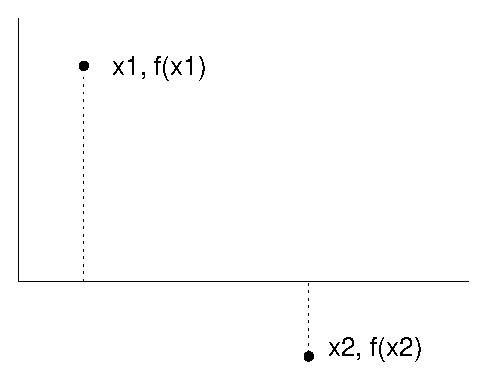
\includegraphics[height=1.5in]{figs/secant.eps}}

If this was all you knew about $f$, where would you go looking for
a zero?  If you said ``halfway between $x_1$ and $x_2$,'' then
congratulations!  You just invented a numerical method called
bisection!

If you said, ``I would connect the dots with a straight line
and compute the zero of the line,'' then
congratulations!  You just invented the secant method!

And if you said, ``I would evaluate $f$ at a third point, find the
parabola that passes through all three points, and compute the zeros
of the parabola,'' then... well, you probably didn't say that.

Finally, if you said, ``I would use a built-in MATLAB function that
combines the best features of several efficient and robust
numerical methods,'' then you are ready to go on to the next section.


\section{{\tt fzero}}
\label{fzero}

{\tt fzero} is a built-in MATLAB function that
combines the best features of several efficient and robust
numerical methods.

In order to use {\tt fzero}, you have to define a MATLAB function
that computes the error function you derived from the original
nonlinear equation, and you have to provide an initial guess at
the location of a zero.

We've already seen an example of an error function:

\begin{verbatim}
function res = error_func(x)
    res = x^2 - 2*x -3;
end
\end{verbatim}

You can call {\tt error\_func} from the Command Window, and
confirm that there are zeros at 3 and -1.

\begin{verbatim}
>> error_func(3)
ans = 0

>> error_func(-1)
ans = 0
\end{verbatim}

But let's pretend that we don't know exactly where
the roots are; we only know that one of them is near 4.  Then
we could call {\tt fzero} like this:

\begin{verbatim}
>> fzero(@error_func, 4)
ans = 3.0000
\end{verbatim}

Success!  We found one of the zeros.

The first argument is a
{\bf function handle} that names the M-file that evaluates
the error function.  The {\tt @} symbol allows us to name the
function without calling it.  The interesting thing here is
that you are not actually calling {\tt error\_func} directly;
you are just telling {\tt fzero} where it is.  In turn, {\tt fzero}
calls your error function---more than once, in fact.

The second argument is the initial guess.  If we provide a different
initial guess, we get a different root (at least sometimes).

\begin{verbatim}
>> fzero(@error_func, -2)
ans = -1
\end{verbatim}

Alternatively, if you know two values that bracket the root,
you can provide both:

\begin{verbatim}
>> fzero(@error_func, [2,4])

ans = 3
\end{verbatim}

The second argument here is actually a vector that contains two
elements.  The bracket operator is a convenient way (one of several)
to create a new vector. 

You might be curious to know how many times {\tt fzero} calls your
function, and where.  If you modify {\tt error\_func} so that it displays
the value of {\tt x} every time it is called and then run {\tt fzero}
again, you get:

\begin{verbatim}
>> fzero(@error_func, [2,4])
x = 2
x = 4
x = 2.75000000000000
x = 3.03708133971292
x = 2.99755211623500
x = 2.99997750209270
x = 3.00000000025200
x = 3.00000000000000
x = 3
x = 3
ans = 3
\end{verbatim}

Not surprisingly, it starts by computing $f(2)$ and $f(4)$.  After
each iteration, the interval that brackets the root gets smaller;
{\tt fzero} stops when the interval is so small that the estimated
zero is correct to 16 digits.  If you
don't need that much precision, you can tell {\tt fzero} to give
you a quicker, dirtier answer (see the documentation for details).


\section{What could go wrong?}

The most common problem people have with {\tt fzero} is leaving
out the {\tt @}.  In that case, you get something like:

\begin{verbatim}
>> fzero(error_func,[2,4])
Not enough input arguments.

Error in error_func (line 2)
    res = x^2 - 2*x -3;
\end{verbatim}

The error occurs as MATLAB treats the first argument as a function call, so it calls {\tt error\_func}
with no arguments.  

Another common problem is writing an error function that never
assigns a value to the output variable.  In general, functions should
{\em always} assign a value to the output variable, but MATLAB doesn't
enforce this rule, so it is easy to forget.  For example, if you
write:

\begin{verbatim}
function res = error_func(x)
    y = x^2 - 2*x -3
end
\end{verbatim}

and then call it from the Command Window:

\begin{verbatim}
>> error_func(4)

y = 5
\end{verbatim}

It looks like it worked, but don't be fooled.  This function assigns
a value to {\tt y}, and it displays the result, but when the function
ends, {\tt y} disappears along with the function's workspace.
If you try to use it with {\tt fzero}, you get

\begin{verbatim}
>> fzero(@error_func,[2,4])

y =

    -3

Error using fzero (line 231)
FZERO cannot continue because user-supplied function_handle ==> 
error_func failed with the error below.

Output argument "res" (and maybe others) not assigned during call
to "error_func".
\end{verbatim}

If you read it carefully, this is a pretty good error message
(with the quibble that ``output argument'' is not a good synonym
for ``output variable'').

You would have seen the same error message when you called {\tt
error\_func} from the interpreter, if only you had assigned the result
to a variable:

\begin{verbatim}
>> x = error_func(4)

y =

     5

Output argument "res" (and maybe others) not assigned during 
call to "error_func".
\end{verbatim}

You can avoid all of this if you remember these two rules:

\begin{itemize}

\item Functions should always assign values to their output
variables\footnote{Well, ok, there are exceptions, including {\tt
find\_triples}.  Functions that don't return a value are sometimes
called ``commands,'' because they do something (like display values or
generate a figure) but either don't have an output variable or don't
make an assignment to it.}.

\item When you call a function, you should always do something with
the result (either assign it to a variable or use it as part of an
expression, etc.).

\end{itemize}

When you write your own functions and use them yourself, it is easy
for mistakes to go undetected.  But when you use your functions with
MATLAB functions like {\tt fzero}, you have to get it right!

Yet another thing that can go wrong: if you provide an interval for the
initial guess and it doesn't actually contain a root, you get

\begin{verbatim}
>> fzero(@error_func,[0,1])
Error using fzero (line 272)
The function values at the interval endpoints must differ in sign.
\end{verbatim}

There is one other thing that can go wrong when you use {\tt fzero}, but
this one is less likely to be your fault.  It is possible that {\tt fzero}
won't be able to find a root.

{\tt fzero} is generally pretty robust, so you may never have a
problem, but you should remember that there is no guarantee that {\tt
fzero} will work, especially if you provide a single value as an
initial guess.  Even if you provide an interval that brackets a root,
things can still go wrong if the error function is discontinuous.


\section{Finding an initial guess}

The better your initial guess (or interval) is, the more likely
it is that {\tt fzero} will work, and the fewer iterations it will
need.

When you are solving problems in the real world, you will usually
have some intuition about the answer.  This intuition is often enough
to provide a good initial guess for zero-finding.

Another approach is to plot the function and see if you can
approximate the zeros visually.  If you have a function, like
{\tt error\_func} that takes a scalar input variable and returns
a scalar output variable, you can plot it with {\tt ezplot}:

\begin{verbatim}
>> ezplot(@error_func, [-2,5])
\end{verbatim}

The first argument is a function handle; the second is the 
interval you want to plot the function in.

By default {\tt ezplot} calls your function 100 times (each time
with a different value of {\tt x}, of course).  So you probably want
to make your function silent before you plot it.

\section{More name collisions}

Functions and variables occupy the same ``name-space,'' which means
that whenever a name appears in an expression, MATLAB starts by looking
for a variable with that name, and if there isn't one, it looks for
a function.

As a result, if you have a variable with the same name as a function,
the variable {\bf shadows} the function.  For example, if you assign
a value to {\tt sin}, and then try to use the {\tt sin} function, you
{\em might} get an error:

\begin{verbatim}
>> sin = 3;
>> x = 5;
>> sin(x)
Index exceeds matrix dimensions.
\end{verbatim}

In this example, the problem is clear.  Since the value of {\tt sin}
is a scalar, and a scalar is really a 1x1 matrix, MATLAB tries to
access the 5th element of the matrix and finds that there isn't one.
Of course, if there were more distance between the assignment
and the ``function call,'' this message would be pretty confusing.

But the only thing worse than getting an error message is {\em not}
getting an error message.  If the value of {\tt sin} was a vector,
or if the value of {\tt x} was smaller, you would really
be in trouble.

\begin{verbatim}
>> sin = 3;
>> sin(1)

ans = 3
\end{verbatim}

Just to review, the sine of 1 is not 3!

The converse error can also happen if you try to access an
undefined variable that also happens to be the name of a function.
For example, if you have a function named {\tt f}, and then
try to increment a variable named {\tt f} (and if you forget to
initialize {\tt f}), you get

\begin{verbatim}
>> f = f+1
Undefined function or variable 'f'.
\end{verbatim}

At least, that's what you get if you are lucky.  If this happens
inside a function, MATLAB tries to call {\tt f} as a function,
and you get this

\begin{verbatim}
>> f = f+1
Not enough input arguments.

Error in f (line 3)
y = x^2 - a
\end{verbatim}

There is no universal way to avoid these kind of
collisions, but you can improve your chances by choosing
variable names that don't shadow existing functions, and by
choosing function names that you are unlikely to use as variables.
That's why in Section~\ref{notation}, I called the error function
{\tt error\_func} rather than {\tt f}.  I often give functions
names that end in {\tt func}, so that helps, too.


\section{Debugging in four acts}

When you are debugging a program, and especially if you are
working on a hard bug, there are four things to try:

\begin{description}

\item[reading:] Examine your code, read it back to yourself, and
check that it means what you meant to say.

\item[running:] Experiment by making changes and running different
versions.  Often if you display the right thing at the right place
in the program, the problem becomes obvious, but sometimes you have to
spend some time to build scaffolding.

\item[ruminating:] Take some time to think!  What kind of error
is it: syntax, run-time, logical?  What information can you get from
the error messages, or from the output of the program?  What kind of
error could cause the problem you're seeing?  What did you change
last, before the problem appeared?

\item[retreating:] At some point, the best thing to do is back
off, undoing recent changes, until you get back to a program that
works, and that you understand.  Then you can starting rebuilding.

\end{description}

Beginning programmers sometimes get stuck on one of these activities
and forget the others.  Each activity comes with its own failure
mode.

For example, reading your code might help if the problem is a
typographical error, but not if the problem is a conceptual
misunderstanding.  If you don't understand what your program does, you
can read it 100 times and never see the error, because the error is in
your head.

Running experiments can help, especially if you run small, simple
tests.  But if you run experiments without thinking or reading your
code, you might fall into a pattern I call ``random walk programming,''
which is the process of making random changes until the program
does the right thing.  Needless to say, random walk programming
can take a long time.

The way out is to take more time to think.  Debugging is like an
experimental science.  You should have at least one hypothesis about
what the problem is.  If there are two or more possibilities, try to
think of a test that would eliminate one of them.

Taking a break sometimes helps with the thinking.  So does talking.
If you explain the problem to someone else (or even yourself), you
will sometimes find the answer before you finish asking the question.

But even the best debugging techniques will fail if there are too many
errors, or if the code you are trying to fix is too big and
complicated.  Sometimes the best option is to retreat, simplifying the
program until you get to something that works, and then rebuild.

Beginning programmers are often reluctant to retreat, because
they can't stand to delete a line of code (even if it's wrong).
If it makes you feel better, copy your program into another file
before you start stripping it down.  Then you can paste the pieces
back in a little bit at a time.

To summarize, here's the Ninth Theorem of debugging:

\begin{quote}
Finding a hard bug requires reading, running, ruminating, and
sometimes retreating.  If you get stuck on one of these activities,
try the others.
\end{quote}



\section{Glossary}

\begin{description}

\item[analytic solution:] A way of solving an equation by performing
algebraic operations and deriving an explicit way to
compute a value that is only known implicitly.

\item[numerical solution:] A way of solving an equation by finding
a numerical value that satisfies the equation, often approximately.

\item[numerical method:] A method (or algorithm) for generating
a numerical solution.

\item[map:] A correspondence between the elements of one set (the
range) and the elements of another (the domain).  You can think of
sequences, vectors and functions as different kinds of maps.

\item[range:] The set of values a map maps from.

\item[domain:] The set of values a map maps to.

\item[discrete set:] A set, like the integers, whose elements are
countable.

\item[continuous set:] A set, like the real numbers, whose elements
are not countable.  You can think of floating-point numbers as a
continuous set.

\item[zero (of a function):] A value in the range of a function that
maps to 0.

\item[function handle:] In MATLAB, a function handle is a way of
referring to a function by name (and passing it as an argument)
without calling it.

\item[shadow:] A kind of name collision in which a new definition
causes an existing definition to become invisible.  In MATLAB,
variable names can shadow built-in functions (with hilarious results). 

\end{description}

\section{Exercises}

\begin{ex}

\begin{enumerate}

\item Write a function called {\tt cheby6} that evaluates the
6th Chebyshev polynomial.  It should take an input variable, 
$x$, and return

\begin{equation}
32 x^6 - 48 x^4 + 18 x^2 - 1
\end{equation}

\item Use {\tt ezplot} to display a graph of this function in the
interval from 0 to 1.  Estimate the location of any zeros in this
range.

\item Use {\tt fzero} to find as many different roots as you can.
Does {\tt fzero} always find the root that is closest to the initial
guess?

\end{enumerate}
\end{ex}


\begin{ex}
\label{duck}

The density of a duck, $\rho$, is $0.3 g / cm^3$ (0.3 times the
density of water).

The volume of a sphere\footnote{This example is adapted from Gerald
and Wheatley, {\em Applied Numerical Analysis}, Fourth Edition,
Addison-Wesley, 1989.} with radius $r$ is $\frac{4}{3} \pi r^3$.

If a sphere with radius $r$ is submerged in water to a depth $d$, the
volume of the sphere below the water line is 

\[ volume = \frac{\pi}{3} (3r d^2 - d^3) \quad 
\mbox{as long as} \quad d < 2 r \]

An object floats at the level where the weight of the displaced water
equals the total weight of the object.

Assuming that a duck is a sphere with radius 10 cm, at what depth does
a duck float?

Here are some suggestions about how to proceed:

\begin{itemize}

\item Write an equation relating $\rho$, $d$ and $r$.

\item Rearrange the equation so the right-hand side is zero.
Our goal is to find values of $d$ that are roots of this equation.

\item Write a MATLAB function that evaluates this function.  Test it,
   then make it a quiet function.

\item Make a guess about the value of $d_0$ to use as a starting place.

\item Use {\tt fzero} to find a root near $d_0$.

\item Check to make sure the result makes sense.  In particular,
   check that $d < 2 r$, because otherwise the volume equation
   doesn't work!

\item Try different values of $\rho$ and $r$ and see if you get the
effect you expect.  What happens as $\rho$ increases?  Goes to
infinity?  Goes to zero?  What happens as $r$ increases?  Goes to
infinity?  Goes to zero?

\end{itemize}


\end{ex}

% for another time, figure out how to use fzero to find zeros of...

%\item The Riemann zeta function can be written

%\[ zeta \equiv w \to sum_{k=1}^\infty k^w \]

%where $w$ is a complex number.  If you are not familiar with
%complex numbers, you should skip this problem.







% chap07
\chapter{Functions of vectors}


\section{Functions and files}
\label{funfiles}

So far we have only put one function in each file.  It is also
possible to put more than one function in a file, but only the first
one, the {\bf top-level function} can be called from the Command
Window.  The other {\bf helper functions} can be called from anywhere
inside the file, but not from any other file.

Large programs almost always require more than one function; keeping
all the functions in one file is convenient, but it makes debugging
difficult because you can't call helper functions from the Command
Window.

To help with this problem, I often use the top-level function
to develop and test my helper functions.  For example, to write
a program for Exercise~\ref{duck}, I would create a file named
{\tt duck.m} and start with a top-level function named {\tt duck}
that takes no input variables and returns no output value.

Then I would write a function named {\tt error\_func} to
evaluate the error function for {\tt fzero}.  To test
{\tt error\_func} I would call it from {\tt duck} and then
call {\tt duck} from the Command Window.

Here's what my first draft might look like:

\begin{verbatim}
function res = duck()
    error = error_func(10)
end

function res = error_func(h)
    rho = 0.3;      % density in g / cm^3
    r = 10;         % radius in cm
    res = h;
end
\end{verbatim}

The line {\tt res = h} isn't finished yet, but this
is enough code to test.
Once I finished and tested {\tt error\_func}, I would modify
{\tt duck} to use {\tt fzero}.

For this problem I might only need two functions, but if there
were more, I could write and test them one at a time, and then
combine them into a working program.



\section{Physical modeling}
\label{modeling}

Most of the examples so far have been about mathematics;
Exercise~\ref{duck}, the ``duck problem,'' is the first example we
have seen of a physical system.  If you didn't work on this exercise,
you should at least go back and read it.

This book is supposed to be about {\bf physical modeling}, so it might
be a good idea to explain what that is.  Physical modeling is a process
for making predictions about physical systems and explaining their
behavior.  A {\bf physical system} is something in the real
world that we are interested in, like a duck.

The following figure shows the steps of this process:

\beforefig \centerline{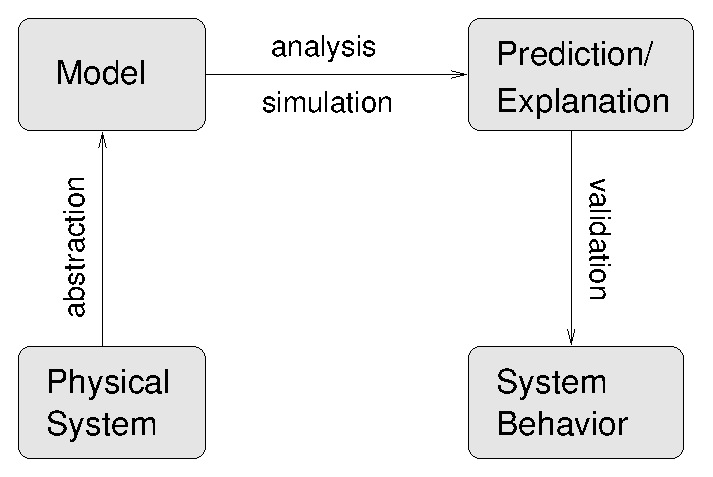
\includegraphics[height=1.5in]{figs/model.eps}}

A {\bf model} is a simplified description of a physical system.  The
process of building a model is called {\bf abstraction}.  In this
context, ``abstract'' is the opposite of ``realistic;'' an abstract
model bears little direct resemblance to the physical system it
models, in the same way that abstract art does not directly depict
objects in the real world.  A realistic model is one that includes
more details and corresponds more directly to the real world.

Abstraction involves making justified decisions about which factors to
include in the model and which factors can be simplified or ignored.
For example, in the duck problem, we took into account the density of
the duck and the buoyancy of water, but we ignored the buoyancy of the
duck due to displacement of air and the dynamic effect of paddling
feet.  We also simplified the geometry of the duck by assuming that
the underwater parts of a duck are similar to a segment of a sphere.
And we used coarse estimates of the size and weight of the duck.

Some of these decisions are justifiable.  The density of the duck
is much higher than the density of air, so the effect of buoyancy
in air is probably small.  Other decisions, like the spherical
geometry, are harder to justify, but very helpful.  The actual
geometry of a duck is complicated; the sphere model makes it possible
to generate an approximate answer without making detailed measurements
of real ducks.

A more realistic model is not necessarily better.  Models are useful
because they can be analyzed mathematically and simulated
computationally.  Models that are too realistic might be difficult to
simulate and impossible to analyze.

A model is successful if it is good enough for its purpose.  If we
only need a rough idea of the fraction of a duck that lies below
the surface, the sphere model is good enough.  If we need a more
precise answer (for some reason) we might need a more realistic
model.

% Einstein's actual quote: ``It can scarcely be denied that the supreme
% goal of all theory is to make the irreducible basic elements as simple
% and as few as possible without having to surrender the adequate
% representation of a single datum of experience.

%     * "On the Method of Theoretical Physics" The Herbert Spencer
%       Lecture, delivered at Oxford (10 June 1933); also published in
%       Philosophy of Science, Vol. 1, No. 2 (April 1934),
%       pp. 163-169. [thanks to Dr. Techie @ www.wordorigins.org and
%       JSTOR]

Checking whether a model is good enough is called {\bf validation}.
The strongest form of validation is to make a measurement of an
actual physical system and compare it to the prediction of a
model.

If that is infeasible, there are weaker forms of validation.  One is
to compare multiple models of the same system.  If they are
inconsistent, that is an indication that (at least) one of them is
wrong, and the size of the discrepancy is a hint about the reliability
of their predictions.

We have only seen one physical model so far, so parts of this
discussion may not be clear yet.  We will come back to these topics
later, but first we should learn more about vectors.



\section{Vectors as input variables}

Since many of the built-in functions take vectors as arguments,
it should come as no surprise that you can write functions that
take vectors.  Here's a simple (silly) example:

\begin{verbatim}
function res = display_vector(X)
    X
end
\end{verbatim}

There's nothing special about this function at all.  The only
difference from the scalar functions we've seen is that I used
a capital letter to remind me that {\tt X} is a vector.

This is another example of a function that doesn't actually have
a return value; it just displays the value of the input variable:

\begin{verbatim}
>> display_vector(1:3)

X = 1     2     3
\end{verbatim}

Here's a more interesting example that encapsulates the code
from Section~\ref{reduce} that adds up the elements of a vector:

\begin{verbatim}
function res = mysum(X)
    total = 0;
    for i=1:length(X)
        total = total + X(i);
    end
    res = total;
end
\end{verbatim}

I called it {\tt mysum} to avoid a collision with the built-in
function {\tt sum}, which does pretty much the same thing.

Here's how you call it from the Command Window:

\begin{verbatim}
>> total = mysum(1:3)

total = 6
\end{verbatim}

Because this function has a return value, I made a
point of assigning it to a variable.


\section{Vectors as output variables}

There's also nothing wrong with assigning a vector to an output
variable.  Here's an example that encapsulates the code from
Section~\ref{apply}:

\begin{verbatim}
function res = myapply(X)
    for i=1:length(X)
        Y(i) = X(i)^2;
    end
    res = Y;
end
\end{verbatim}

Ideally I would have changed the name of the output variable to
{\tt Res}, as a reminder that it is supposed to get a vector value,
but I didn't.

Here's how {\tt myapply} works:

\begin{verbatim}
>> V = myapply(1:3)

V = 1     4     9
\end{verbatim}

\begin{ex}
Write a function named {\tt find\_target} that
encapsulates the code, from Section~\ref{search}, that finds the
location of a target value in a vector.
\end{ex}


\section{Vectorizing your functions}

Functions that work on vectors will almost always work on scalars
as well, because MATLAB considers a scalar to be a vector with
length 1.

\begin{verbatim}
>> mysum(17)

ans = 17

>> myapply(9)

ans = 81
\end{verbatim}

Unfortunately, the converse is not always true.  If you write
a function with scalar inputs in mind, it might not work on vectors.

But it might!  If the operators and functions
you use in the body of your function work on vectors, then your
function will probably work on vectors.

For example, here is the very first function we wrote:

\begin{verbatim}
function res = myfunc (x)
    s = sin(x);
    c = cos(x);
    res = abs(s) + abs(c);
end
\end{verbatim}

And lo!  It turns out to work on vectors:

\begin{verbatim}
>> Y = myfunc(1:3)

Y = 1.3818    1.3254    1.1311
\end{verbatim}

At this point, I want to take a minute to acknowledge that I
have been a little harsh in my presentation of MATLAB, because
there are a number of features that I think make life harder
than it needs to be for beginners.  But here, finally,
we are seeing features that show MATLAB's strengths.

Some of the other functions we wrote don't work on vectors,
but they can be patched up with just a little effort.  For example,
here's {\tt hypotenuse} from Section~\ref{hypotenuse}:

\begin{verbatim}
function res = hypotenuse(a, b)
    res = sqrt(a^2 + b^2);
end
\end{verbatim}

This doesn't work on vectors because the \verb+^+ operator
tries to do matrix exponentiation, which only works on
square matrices.

\begin{verbatim}
>> hypotenuse(1:3,1:3)
Error using  ^ 
Inputs must be a scalar and a square matrix.
To compute elementwise POWER, use POWER (.^) instead.

Error in hypotenuse (line 2)
    res = sqrt(a^2 + b^2);
\end{verbatim}

But if you replace \verb+^+ with the elementwise operator
\verb+.^+, it works!

\begin{verbatim}
>> A = [3,5,8];
>> B = [4,12,15];
>> C = hypotenuse(A, B)

C = 5    13    17
\end{verbatim}
 
In this case, it matches up corresponding elements from the two
input vectors, so the elements of {\tt C} are the hypotenuses of
the pairs $(3,4)$, $(5,12)$ and $(8,15)$, respectively.

In general, if you write a function using only elementwise
operators and functions that work on vectors, then the new
function will also work on vectors.


\section{Sums and differences}

Another common vector operation is {\bf cumulative sum}, which takes a
vector as an input and computes a new vector that contains all of the
partial sums of the original.  In math notation, if $V$ is the
original vector, then the elements of the cumulative sum, $C$, are:

\[ C_i = \sum_{j=1}^i V_j \]

In other words, the $i$th element of $C$ is the sum of the first
$i$ elements from $V$.  MATLAB provides a function named {\tt cumsum}
that computes cumulative sums:

\begin{verbatim}
>> V = 1:5

V = 1     2     3     4     5

>> C = cumsum(V)

C = 1     3     6    10    15
\end{verbatim}

\begin{ex}
Write a function named {\tt cumulative\_sum} that uses
a loop to compute the cumulative sum of the input vector.
\end{ex}

The inverse operation of {\tt cumsum} is {\tt diff}, which computes
the difference between successive elements of the input vector.

\begin{verbatim}
>> D = diff(C)

D = 2     3     4     5
\end{verbatim}

Notice that the output vector is shorter by one than the input
vector.  As a result, MATLAB's \index{version} of {\tt diff} is not
exactly the inverse of {\tt cumsum}.  If it were, then we would
expect {\tt cumsum(diff(X))} to be {\tt X}:

\begin{verbatim}
>> cumsum(diff(V))

ans = 1     2     3     4
\end{verbatim}

But it isn't.

\begin{ex}
Write a function named {\tt mydiff} that computes the
inverse of {\tt cumsum}, so that {\tt cumsum(mydiff(X))} and
{\tt mydiff(cumsum(X))} both
return {\tt X}.
\end{ex}


\section{Products and ratios}

The multiplicative \index{version} of {\tt cumsum} is {\tt cumprod},
which computes the {\bf cumulative product}.  In math notation,
that's:

\[ P_i = \prod_{j=1}^i V_j \]

In MATLAB, that looks like:

\begin{verbatim}
>> V = 1:5

V = 1     2     3     4     5

>> P = cumprod(V)

P = 1     2     6    24   120
\end{verbatim}

\begin{ex}
Write a function named {\tt cumulative\_prod} that uses
a loop to compute the cumulative product of the input \index{vector}.
\end{ex}

MATLAB doesn't provide the multiplicative \index{version}
of {\tt diff}, which would be called {\tt ratio}, and which would
compute the ratio of successive elements of the input \index{vector}.

\begin{ex}
Write a function named {\tt myratio} that computes the
inverse of {\tt cumprod}, so that {\tt cumprod(myratio(X))} and
{\tt myratio(cumprod(X))} both
return {\tt X}.

You can use a loop, or if you want to be clever, you can take
advantage of the fact that $e^{\ln a + \ln b} = a b$.

If you apply {\tt myratio} to a \index{vector} that contains Fibonacci
numbers, you can confirm that the ratio of successive elements
converges on the golden ratio, $(1+\sqrt{5})/2$ (see
Exercise~\ref{fibratio}).
\end{ex}



\section{Existential quantification}

It is often useful to check the elements of a \index{vector} to see if there
are any that satisfy a condition.  For example, you might want to
know if there are any positive elements.  In logic, this condition
is called {\bf existential quantification}, and it is denoted with
the symbol $\exists$, which is pronounced ``there exists.''  For example,
this expression

\[ \exists x \mbox{~in~} S: x>0 \]

means, ``there exists some element $x$ in the set $S$ such that
$x>0$.''  In MATLAB it is natural to express this idea with a logical
function, like {\tt exists}, that returns 1 if there is such an
element and 0 if there is not.

\begin{verbatim}
function res = exists(X)
    for i=1:length(X)
        if X(i) > 0
            res = 1;
            return
        end
    end
    res = 0;
end
\end{verbatim}

We haven't seen the {\tt return} statement before; it is similar
to {\tt break} except that it breaks out of the whole function, not
just the loop.  That behavior is what we want here because as soon
as we find a positive element, we know the answer (it exists!) and
we can end the function immediately without looking at the rest
of the elements.

If we exit at the end of the loop, that means we didn't find what
we were looking for (because if we had, we would have hit the
{\tt return} statement).



\section{Universal quantification}

Another common operation on \index{vector}s is to check whether {\em all}
of the elements satisfy a condition, which is known to
logicians as {\bf universal quantification} and denoted with
the symbol $\forall$ which is pronounced ``for all.''  So this
expression

\[ \forall x \mbox{~in~} S: x>0 \]

means ``for all elements, $x$, in the set $S$, $x>0$.''

A slightly silly way to evaluate this expression in MATLAB is to
count the number of elements that satisfy the condition.
A better way is to reduce the problem to
existential quantification; that is, to rewrite

\[ \forall x \mbox{~in~} S: x>0 \]

as

\[ \sim \exists x \mbox{~in~} S: x \le 0 \]

Where $\sim \exists$ means ``does not exist.''
In other words, checking that all the elements are positive is
the same as checking that there are no elements 
that are non-positive.

\begin{ex}
Write a function named {\tt forall} that
takes a \index{vector} and returns 1 if all of the elements are positive
and 0 if there are any non-positive elements.
\end{ex}




\section{Logical \index{vector}s}

When you apply a logical operator to a \index{vector}, the result is a {\bf
logical \index{vector}}; that is, a \index{vector} whose elements are the logical
values 1 and 0.

\begin{verbatim}
>> V = -3:3

V = -3    -2    -1     0     1     2     3

>> L = V>0

L =  0     0     0     0     1     1     1
\end{verbatim}

In this example, {\tt L} is a logical \index{vector} whose elements
correspond to the elements of {\tt V}.  For each positive element of
{\tt V}, the corresponding element of {\tt L} is 1.

Logical \index{vector}s can be used like flags to store the state of
a condition.  They are also often used with the {\tt find} function,
which takes a logical \index{vector} and returns a \index{vector} that contains
the indices of the elements that are ``true.''

Applying {\tt find} to {\tt L} yields

\begin{verbatim}
>> find(L)

ans = 5     6     7
\end{verbatim}

which indicates that elements 5, 6 and 7 have the value 1.

If there are no ``true'' elements, the result is an empty \index{vector}.

\begin{verbatim}
>> find(V>10)

ans =

   Empty matrix: 1-by-0
\end{verbatim}

This example computes the logical \index{vector} and passes it as an
argument to {\tt find} without assigning it to an intermediate
variable.  You can read this \index{version} abstractly as ``find
the indices of elements of {\tt V} that are greater than 10.''

We can also use {\tt find} to write {\tt exists} more concisely:

\begin{verbatim}
function res = exists(X)
    L = find(X>0)
    res = length(L) > 0
end
\end{verbatim}

\begin{ex}
Write a \index{version} of {\tt forall} using {\tt find}.
\end{ex}


\section{Glossary}

\begin{description}

\item[top-level function:]  The first function in an M-file;
it is the only function that can be called from the Command
Window or from another file.

\item[helper function:] A function in an M-file that is not
the top-level function; it only be called from another function
in the same file.

\item[physical modeling:] A process
for making predictions about physical systems and explaining their
behavior.

\item[physical system:] Something in the real world that we are
interested in studying.

\item[model :] A simplified description of a
physical system that lends itself to analysis or simulation.

\item[abstraction:] The process of building a model by making
decisions about what factors to simplify or ignore.

\item[validation:] Checking whether a model is adequate for its
purpose.

\item[existential quantification:] A logical condition that expresses
the idea that ``there exists'' an element of a set with a certain
property.

\item[universal quantification:] A logical condition that expresses
the idea that all elements of a set have a certain property.

\item[logical \index{vector}:] A \index{vector}, usually the result of applying a logical
operator to a \index{vector}, that contains logical values 1 and 0. 


\end{description}

%\section{Exercises}

%\begin{ex}
%\end{ex}


% chap08
\chapter{Ordinary Differential Equations}


\section{Differential equations}

A {\bf differential equation} (DE) is an equation that describes the
derivatives of an unknown function.  ``Solving a DE'' means finding a
function whose derivatives satisfy the equation.

For example, when bacteria grow in particularly bacteria-friendly
conditions, the rate of growth at any point in time is proportional to
the current population.  What we might like to know is the population
as a function of time.  Toward that end, let's define $f$ to be a
function that maps from time, $t$, to population $y$, such that $y = f(t)$.  We don't
know what it is, but we can write a differential equation
that describes it:

\[ \frac{df}{dt} = a f \]

where $a$ is a constant that characterizes how quickly the population
increases.

Notice that both sides of the equation are functions.  To say that
two functions are equal is to say that their values are equal at
all times.  In other words:

\[ \forall t: \frac{df}{dt}(t) = a f(t) \]

This is an {\bf ordinary} differential equation (ODE) because all the
derivatives involved are taken with respect to the
same variable.  If the equation related derivatives with respect to
different variables (partial derivatives), it would be a {\bf partial}
differential equation.

This equation is {\bf first order} because it involves only first
derivatives.  If it involved second derivatives, it would be second order,
and so on.

This equation is {\bf linear} because each term involves $t$, $f$ or
$df/dt$ raised to the first power; if any of the terms involved
products or powers of $t$, $f$ and $df/dt$ it would be
nonlinear.

Linear, first order ODEs can be solved analytically; that is, we
can express the solution as a function of $t$.
This particular ODE has an infinite number of solutions, but
they all have this form:

\[ f(t) = b e^{at} \]

For any value of $b$, this function satisfies the ODE.  If
you don't believe me, take its derivative and check.

If we know the population of bacteria at a particular point in time,
we can use that additional information to determine which of the
infinite solutions is the (unique) one that describes a particular
population over time.

For example, if we know that $f(0) = 5$ billion cells, then we
can write

\[ f(0) = 5 = b e^{a 0} \]

and solve for $b$, which is 5.  That determines what we wanted
to know:

\[ f(t) = 5 e^{at} \]

The extra bit of information that determines $b$ is called
the {\bf initial condition} (although it isn't always specified
at $t=0$).

Unfortunately, most interesting physical systems are described by
nonlinear DEs, most of which can't be solved analytically.  The
alternative is to solve them numerically.


\section{Euler's method}

The simplest numerical method for ODEs is Euler's method.  Here's a
test to see if you are as smart as Euler.  Let's say that you
arrive at time $t$ and measure the current population, $y$, and
the rate of change, $r$.  What do you think the population will
be after some period of time $\Delta t$ has elapsed?

If you said $y + r \Delta t$, congratulations!  You just invented
Euler's method (but you're still not as smart as Euler).

This estimate is based on the assumption that $r$ is constant, but
in general it's not, so we only expect the estimate to be good if
$r$ changes slowly and $\Delta t$ is small.

But let's assume (for now) that the ODE we are interested in can
be written so that

\[ \frac{df}{dt}(t) = g(t, y) \]

where $g$ is some function that maps $(t, y)$ onto $r$;
that is, given the time and current population, it computes the rate
of change.  Then we can advance from one point in time to the
next using these equations:

\begin{eqnarray}
\label{euler1}
T_{n+1} = T_n + \Delta t           \\
\label{euler2}
F_{n+1} = F_n + g(T_n,f(T_n))~\Delta t
\end{eqnarray}

Here $\{T_i\}$ is a sequence of times where we estimate the value
of $f$, and $\{F_i\}$ is the sequence of estimates.  For each
index $i$, $F_i$ is an estimate of $f(T_i)$.
The interval $\Delta t$ is called the {\bf time step}.

Assuming that we start at $t=0$ and we have an initial condition $f(0)
= y_0$ (where $y_0$ denotes a particular, known value), we set
$T_1 = 0$ and $F_1 = y_0$, and then use 
Equations~\ref{euler1} and~\ref{euler2} to
compute values of $T_i$ and $F_i$ until $T_i$ 
gets to the value of $t$ we are interested in.

If the rate doesn't change too fast and the time step isn't
too big, Euler's method is accurate enough for most purposes.  One
way to check is to run it once with time step $\Delta t$ and then run it
again with time step $\Delta t/2$.  If the results are the same, they are
probably accurate; otherwise, cut the time step again.

Euler's method is {\bf first order}, which means that each time you
cut the time step in half, you expect the estimation error to drop by
half.  With a second-order method, you expect the error to drop by a
factor of 4; third-order drops by 8, etc.  The price of higher order
methods is that they have to evaluate $g$ more times per time step.


\section{Another note on notation}

There's a lot of math notation in this chapter so I want to pause to
review what we have so far.  Here are the variables and their meanings,
which are sorted according to their types:

\begin{tabular}{|l|l|l|}
\hline
Name     &  Meaning             &  Type  \\
\hline \hline
$t$     &  time                 & scalar variable \\\hline
$\Delta t$  &  time step            & scalar constant \\\hline

$y$     &  population           & scalar variable \\\hline
$r$     &  rate of change       & scalar variable \\\hline

$f$     &  The unknown function specified,    &  function, f(t): $t \to y$  \\
        &  implicitly, by an ODE.             &    \\\hline

$df/dt$  &  The first time derivative of $f$  &  function, df/dt(t): $t \to r$  \\ \hline

$g$     &  A ``rate function,'' derived from     &  \\
        &  the ODE, that computes rate of     &  function, g(t,y): $t, y \to r$  \\
        &  change for any $t$, $y$.           &   \\\hline

$T$     & a sequence of times, $t$, where   & sequence \\
              & we estimate $f(t)$    &           \\\hline
$F$     & a sequence of estimates for $f(t)$  & sequence \\
\hline
\end{tabular}

So $f$ is a function that computes the population as a function of
time, $f(t)$ is the function evaluated at a particular time, and if we
assign $f(t)$ to a variable, we usually call that variable $y$.

Similarly, $g$ is a ``rate function'' that computes the rate of change as a
function of time and population.  If we assign $g(t,y)$ to a variable,
we call it $r$.

$df/dt$ is the first derivative of $f$, and it maps from $t$ to a
rate.  If we assign $df/dt(t)$ to a variable,
we call it $r$.

It is easy to get $df/dt$ confused with $g$, but notice that they are
not even the same type.  $g$ is more general: it can compute the rate
of change for any (hypothetical) population at any time; $df/dt$
is more specific: it is the actual rate of change at time $t$, given
that the population is $f(t)$.


\section{{\tt ode45}}
\label{ode45}

A limitation of Euler's method is that the time step is constant from
one iteration to the next.  But some parts of the solution are
harder to estimate than others; if the time step is small enough to
get the hard parts right, it is doing more work than necessary on the
easy parts.  The ideal solution is to adjust the time step as you go
along.  Methods that do that are called {\bf adaptive}, and one of the
best adaptive methods is the Dormand-Prince pair of Runge-Kutta
formulas.  You don't have to know what that means,
because the nice people at Mathworks have implemented it in a function
called {\tt ode45}.  The {\tt ode} stands for ``ordinary differential
equation [solver]'' the 45 indicates that it uses a combination of
4th and 5th order formulas.

In order to use {\tt ode45}, you have to write a MATLAB function
that evaluates $g$ as a function of
$t$ and $y$.

% where did the rats example come from?

As an example, suppose that the rate of population growth for rats
depends on the current population and the availability of food,
which varies over the course of the year.
The governing equation might be something like

\[ \frac{df}{dt}(t) = a f(t) \left[1 + \sin (\omega t) \right] \]
%
where $t$ is time in days and $f(t)$ is the population at time $t$.

$a$ and $\omega$ are {\bf parameters}.  A parameter is a value that
quantifies a physical aspect of the scenario being modeled.  For
example, in Exercise~\ref{duck} we used parameters {\tt rho} and
{\tt r} to quantify the density and radius of a duck.  Parameters are
often constants, but in some models they vary in time.

In this example, $a$ characterizes the reproductive rate, and
$\omega$ is the frequency of a periodic function that describes
the effect of varying food supply on reproduction.

This equation specifies a relationship between a
function and its derivative.  In order to estimate values of
$f$ numerically, we have to transform it into a rate function.

The first step is to introduce a variable,
$y$, as another name for $f(t)$

\[ \frac{df}{dt}(t) = a y \left[1 + \sin (\omega t) \right] \]

This equation means that if we are given $t$ and $y$, we can
compute $df/dt(t)$, which is the rate of change of $f$.
The next step is to express that computation as a function called
$g$:

\[ g(t, y) = a y \left[1 + \sin (\omega t) \right] \]

Writing the function this way is useful because we can use it 
with Euler's method
or {\tt ode45} to estimate values of $f$.  All we have to
do is write a MATLAB function that evaluates $g$.  Here's what
that looks like using the values $a = 0.01$
and $\omega = 2 \pi/365$ (one cycle per year):

\begin{verbatim}
function res = rats(t, y)
    a = 0.01;
    omega = 2 * pi / 365;
    res = a * y * (1 + sin(omega * t));
end
\end{verbatim}

You can test this function from the Command Window by calling it with
different values of {\tt t} and {\tt y}; the result is the rate of
change (in units of rats per day):

\begin{verbatim}
>> r = rats(0, 2)

r = 0.0200
\end{verbatim}

So if there are two rats on January 1, we expect them to reproduce
at a rate that would produce 2 more rats per hundred days. But
if we come back in April, the rate has almost doubled:

\begin{verbatim}
>> r = rats(120, 2)

r = 0.0376
\end{verbatim}

Since the rate is constantly changing, it is not easy to predict
the future rat population, but that is exactly what {\tt ode45} does.
Here's how you would use it:

\begin{verbatim}
>> ode45(@rats, [0, 365], 2)
\end{verbatim}

The first argument is a handle for the function that
computes $g$.  The second argument is the interval we are interested
in, one year.  The third argument is the initial population, $f(0) = 2$.

When you call {\tt ode45} without assigning the result to a variable,
MATLAB displays the result in a figure:

\beforefig \centerline{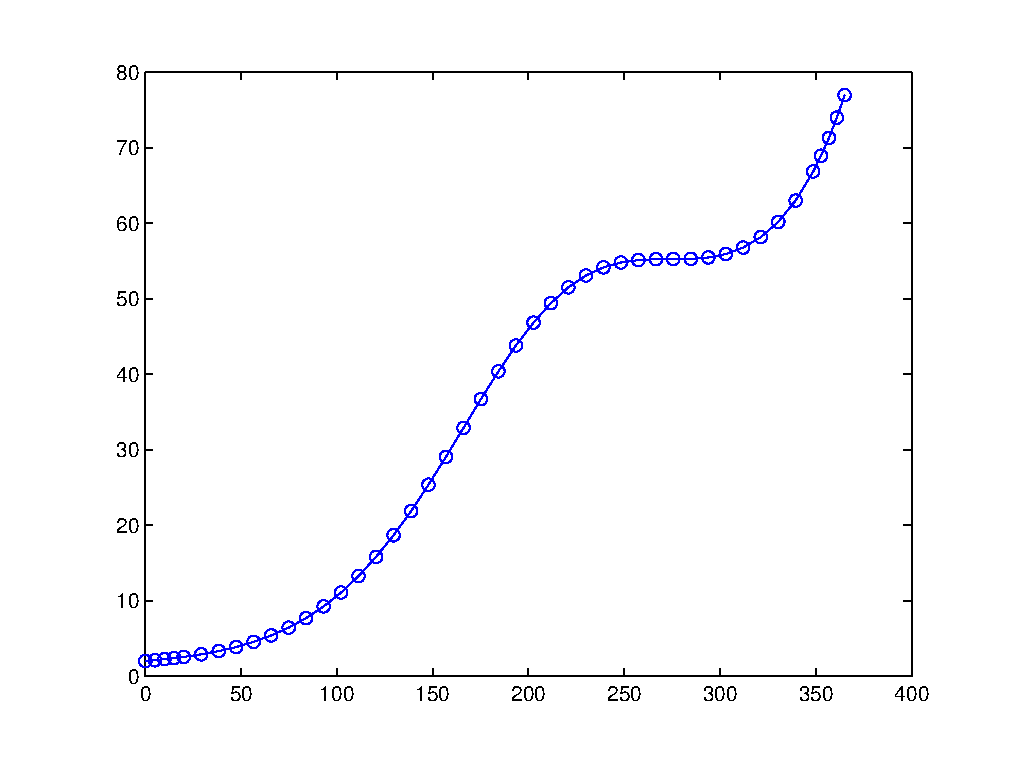
\includegraphics[height=2in]{figs/rats.eps}}

The x-axis shows time from 0 to 365 days; the y-axis shows the rat
population, which starts at 2 and grows to almost 80.  The rate
of growth is slow in the winter and summer, and faster in the
spring and fall, but it also accelerates as the population grows.


\section{Multiple output variables}
\label{rats}

{\tt ode45} is one of many MATLAB functions that return more
than one output variable.  The syntax for calling it and saving
the results is

\begin{verbatim}
>> [T, Y] = ode45(@rats, [0, 365], 2);
\end{verbatim}

The first return value is assigned to {\tt T}; the second is assigned
to {\tt Y}.  Each element of {\tt T} is a time,
$t$, where {\tt ode45} estimated the population; each element of {\tt
Y} is an estimate of $f(t)$.

If you assign the output values to variables,
{\tt ode45} doesn't draw the figure;
you have to do it yourself:

\begin{verbatim}
>> plot(T, Y, 'bo-')
\end{verbatim}

If you plot the elements of {\tt T}, you'll see that the
space between the points is not quite even.  They are closer
together at the beginning of the interval and farther apart at the end.

To see the population at the end of the year, you can display the
last element from each \index{vector}:

\begin{verbatim}
>> [T(end), Y(end)]

ans =

  365.0000   76.9530
\end{verbatim}

{\tt end} is a special word in MATLAB; when it appears as an index,
it means ``the index of the last element.''  You can use it in an
expression, so {\tt Y(end-1)} is the second-to-last element of
{\tt Y}.

How much does the final population change if you double the initial
population?  How much does it change if you double the interval
to two years?  How much does it change if you double the value
of $a$?


\section{Analytic or numerical?}

When you solve an ODE analytically, the result is a function, $f$,
that allows you to compute the population, $f(t)$, for any value of
$t$.  When you solve an ODE numerically, you get two \index{vector}s.  You can
think of these \index{vector}s as a discrete approximation of the continuous
function $f$: ``discrete'' because it is only defined for certain
values of $t$, and ``approximate'' because each value $F_i$
is only an estimate of the true value $f(t)$.

So those are the limitations of numerical solutions.  The primary
advantage is that you can compute numerical solutions to ODEs that
don't have analytic solutions, which is the vast majority
of nonlinear ODEs.

If you are curious to know more about how {\tt ode45} works, you
can modify {\tt rats} to display the points, $(t, y)$, where
{\tt ode45} evaluates $g$.  Here is a simple \index{version}:

\begin{verbatim}
function res = rats(t, y)
    plot(t, y, 'bo')
    a = 0.01;
    omega = 2 * pi / 365;
    res = a * y * (1 + sin(omega * t));
end
\end{verbatim}

Each time {\tt rats} is called, it plots one data point; in order
to see all of the data points, you have to use {\tt hold on}.

\begin{verbatim}
>> clf; hold on
>> [T, Y] = ode45(@rats, [0, 10], 2);
\end{verbatim}
The simple \index{version} of the script shows the output from Day 0 to 10 without label:
\beforefig \centerline{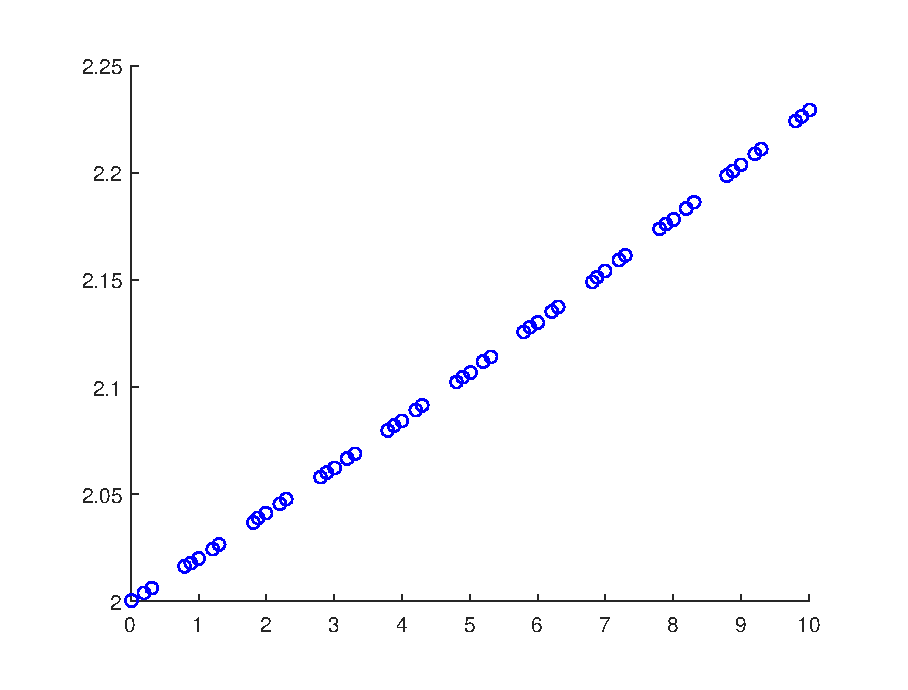
\includegraphics[height=2.2in]{figs/ode45_simple.eps}}

A more comprehensive \index{version} of the script, "rats2.m", can be obtained from the textbook's website\footnote{
\url{https://github.com/AllenDowney/PhysicalModelingInMATLAB/blob/master/code/rats2.m}}.
This script shows part of the output, zoomed in on the range from Day 100 to 170:

\beforefig \centerline{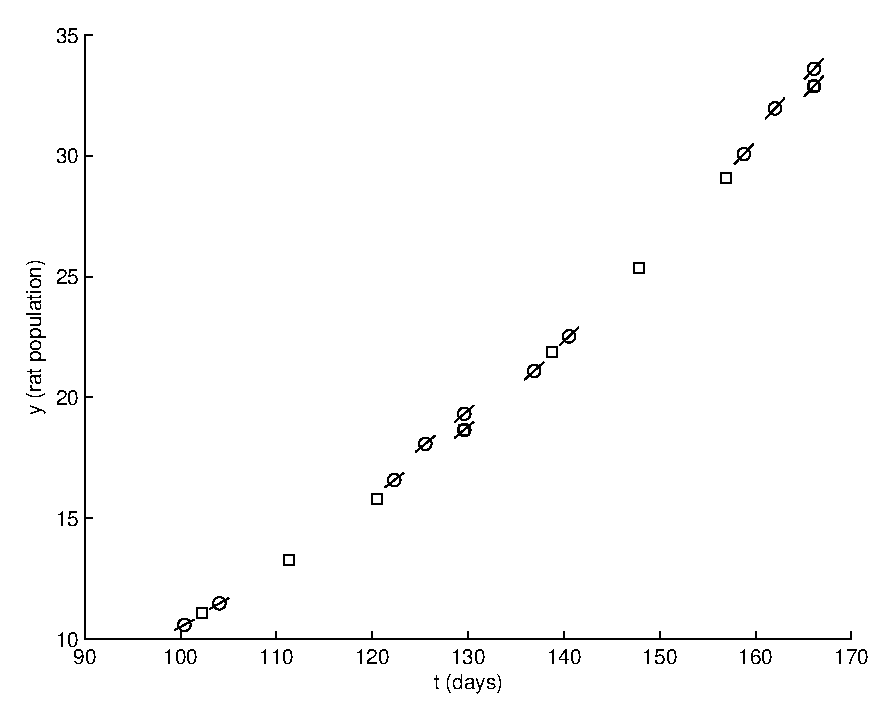
\includegraphics[height=2.2in]{figs/ode45.eps}}

The circles show the points where {\tt ode45} called {\tt rats}.
The lines through the circles show the slope (rate of change) calculated
at each point.  The rectangles show the locations of the estimates
$(T_i, F_i)$.  Notice that {\tt ode45} typically evaluates
$g$ several times for each estimate.  This allows it to improve the
estimates, for one thing, but also to detect places where the errors
are increasing so it can decrease the time step (or the other
way around).


\section{What can go wrong?}

Don't forget the {\tt @} on the function handle.
If you leave it out, MATLAB treats the first argument as a function
call, and calls {\tt rats} without providing arguments.

\begin{verbatim}
>> ode45(rats, [0,365], 2)
Not enough input arguments.

Error in rats (line 4)
    res = a * y * (1 + sin(omega * t));
\end{verbatim}

Again, the error message is confusing, because it looks like the problem
is in {\tt rats}.  You've been warned!

Also, remember that the function you write will be called by
{\tt ode45}, which means it has to have the signature {\tt ode45}
expects: it should take two input variables, {\tt t} and {\tt y},
in that order, and return one output variable, {\tt r}.

If you are working with a rate function like this:

\[ g(t, y) = a y \]

You might be tempted to write this:

\begin{verbatim}
function res = rate_func(y)        % WRONG
    a = 0.1
    res = a * y
end
\end{verbatim}

But that would be wrong.  So very wrong.  Why?  Because
when {\tt ode45} calls {\tt rate\_func}, it provides two arguments.
If you only take one input variable, you'll get an error.  So
you have to write a function that takes {\tt t} as an input
variable, even if you don't use it.

\begin{verbatim}
function res = rate_func(t, y)     % RIGHT
    a = 0.1
    res = a * y
end
\end{verbatim}

Another common error is to write a function that doesn't make
an assignment to the output variable.  If you write something
like this:

\begin{verbatim}
function res = rats(t, y)
    a = 0.01;
    omega = 2 * pi / 365;
    r = a * y * (1 + sin(omega * t))    % WRONG
end
\end{verbatim}

And then call it from {\tt ode45}, you get

\begin{verbatim}
Output argument "res" (and maybe others) not assigned during call
to "rats_8_7".

Error in odearguments (line 87)
f0 = feval(ode,t0,y0,args{:});   % ODE15I sets args{1} to yp0.

Error in ode45 (line 115)
    odearguments(FcnHandlesUsed, solver_name, ode, tspan, y0, 
    options, varargin);
\end{verbatim}

This might be a scary message, but if you read the first line
and ignore the rest, you'll get the idea.

Yet another mistake that people make with {\tt ode45} is leaving
out the brackets on the second argument.  In that case, MATLAB
thinks there are four arguments, and you get

\begin{verbatim}
>> ode45(@rats, 0, 365, 2)
Error using odearguments (line 21)
When the first argument to ode45 is a function handle, the tspan
argument must have at least two elements.

Error in ode45 (line 115)
    odearguments(FcnHandlesUsed, solver_name, ode, tspan, y0, 
    options, varargin);
\end{verbatim}

Again, if you read the first line, you should be able to figure
out the problem ({\tt tspan} stands for ``time span'', which we
have been calling the interval).


\section{Stiffness}

There is yet another problem you might encounter, but if it makes you
feel better, it might not be your fault: the problem you are trying to
solve might be {\bf stiff}\footnote{The following discussion is based
partly on an article from Mathworks available at
\url{http://www.mathworks.com/company/newsletters/news_notes/clevescorner/may03_cleve.html}}.

I won't give a technical explanation of stiffness here, except
to say that for some problems (over some intervals with some initial
conditions) the time step needed to control the error is very small,
which means that the computation takes a long time.  Here's one
example:

\[ \frac{df}{dt} = f^2 - f^3 \]

If you solve this ODE with the initial condition $f(0) = \delta$ over
the interval from 0 to $2/\delta$, with $\delta = 0.01$, you should
see something like this:

\beforefig \centerline{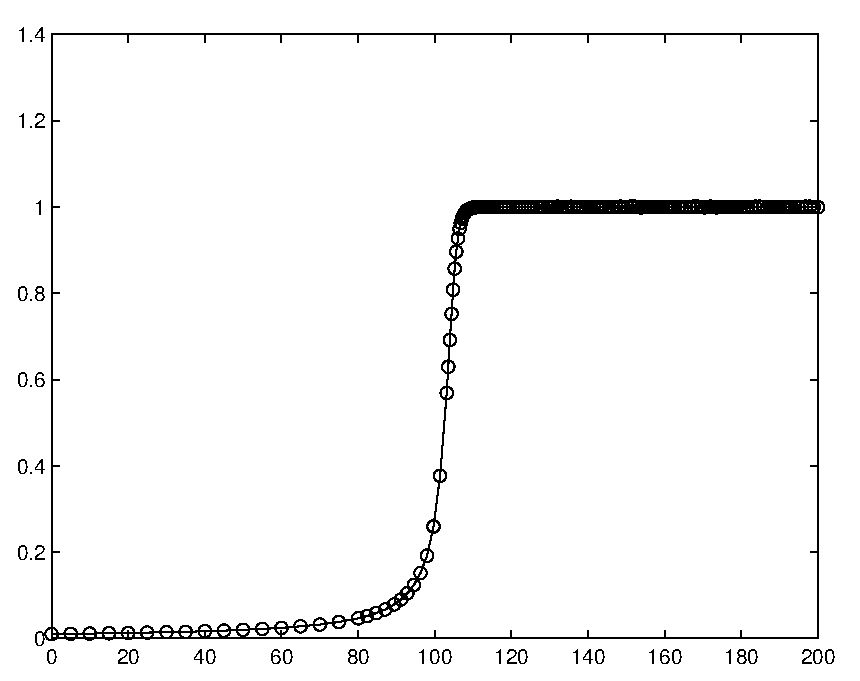
\includegraphics[height=2in]{figs/stiff.eps}}

After the transition from 0 to 1, the time step is very small and the
computation goes slowly.  For smaller values of $\delta$, the
situation is even worse.

In this case, the problem is easy to fix: instead of {\tt ode45} you can
use {\tt ode23s}, an ODE solver that tends to perform well on stiff
problems (that's what the ``s'' stands for).

In general, if you find that {\tt ode45} is taking a long time, you
might want to try one of the stiff solvers.  It won't always solve
the problem, but if the problem is stiffness, the improvement can
be striking.

\begin{ex}
Write a rate function for this ODE and use
{\tt ode45} to solve it with the given initial condition and interval.
Start with $\delta = 0.1$ and decrease it by multiples of 10.  If
you get tired of waiting for a computation to complete, you can 
press the Stop button in the Figure window or press Control-C in
the Command Window.

Now replace {\tt ode45} with {\tt ode23s} and try again!
\end{ex}



\section{Glossary}

\begin{description}

\item[differential equation (DE):] An equation that relates the
derivatives of an unknown function.

\item[ordinary DE:] A DE in which all derivatives are taken with
respect to the same variable.

\item[partial DE:] A DE that includes derivatives with respect to
more than one variable

\item[first order (ODE):] A DE that includes only first derivatives.

\item[linear:] A DE that includes no products or powers of the
function and its derivatives.

\item[time step:] The interval in time between successive estimates
in the numerical solution of a DE.

\item[first order (numerical method):] A method whose error is expected
to halve when the time step is halved.

\item[adaptive:] A method that adjusts the time step to control error.

\item[stiffness:] A characteristic of some ODEs that makes some ODE
solvers run slowly (or generate bad estimates).  Some ODE solvers,
like {\tt ode23s}, are designed to work on stiff problems.

\item[parameter:] A value that appears in a model to quantify some
physical aspect of the scenario being modeled.

\end{description}

\section{Exercises}

\newcommand{\degree}{\ensuremath{^\circ}}

\begin{ex}
Suppose that you are given an 8 ounce cup of coffee at 90 \degree C and
a 1 ounce container of cream at room temperature, which is 20 \degree C.
You have learned from bitter experience that the hottest coffee you
can drink comfortably is 60 \degree C.

Assuming that you take cream in your coffee, and that you would like
to start drinking as soon as possible, are you better off adding
the cream immediately or waiting?  And if you should wait, then how
long?

To answer this question, you have to model the cooling process
of a hot liquid in air.  Hot coffee transfers heat to the environment
by conduction, radiation, and evaporative cooling.  Quantifying these
effects individually would be challenging and unnecessary to answer
the question as posed.

As a simplification, we can use Newton's Law of
Cooling\footnote{\url{https://en.wikipedia.org/wiki/Heat_conduction}}:

\[ \frac{df}{dt} = -r (f - e) \]
%
where $f$ is the temperature of the coffee as a function of time and
$df/dt$ is its time derivative; $e$ is the temperature of the
environment, which is a constant in this case, and $r$ is a parameter
(also constant) that characterizes the rate of heat transfer.

It would be easy to estimate $r$ for a given coffee cup by making
a few measurements over time.  Let's assume that that has been
done and $r$ has been found to be $0.001$ in units of inverse
seconds, $1/s$.

\begin{itemize}

\item Using mathematical notation, write the rate function, $g$,
as a function of $y$, where $y$ is the temperature of the
coffee at a particular point in time.

\item Create an M-file named {\tt coffee} and write a function
called {\tt coffee} that takes no input variables and returns no
output value.  Put a simple statement like {\tt x=5} in the body
of the function and invoke {\tt coffee()} from the Command Window.

\item Add a function called
{\tt rate\_func} that takes {\tt t} and {\tt y} and computes
$g(t,y)$.  Notice that in this case $g$ does not actually
depend on $t$; nevertheless, your function has to take $t$ as
the first input argument in order to work with {\tt ode45}.

Test your function by adding a line like {\tt rate\_func(0,90)}
to {\tt coffee}, the call {\tt coffee} from the Command Window.

\item Once you get {\tt rate\_func(0,90)} working, modify
{\tt coffee} to use {\tt ode45} to compute the temperature
of the coffee (ignoring the cream) for 60 minutes.  Confirm that
the coffee cools quickly at first, then more slowly, and reaches
room temperature (approximately) after about an hour.

\item Write a function called {\tt mix\_func} that computes
the final temperature of a mixture of two liquids.  It should
take the volumes and temperatures of the liquids as parameters.

In general, the final temperature of a mixture depends on the specific
heat of the two
substances\footnote{\url{https://en.wikipedia.org/wiki/Heat_capacity}}.
But if we make the simplifying assumption that coffee and cream
have the same density and specific heat, then the final temperature is
$(v_1 y_1 + v_2 y_2) / (v_1 + v_2)$, where $v_1$ and $v_2$ are
the volumes of the liquids, and $y_1$ and $y_2$ are their
temperatures.

Add code to {\tt coffee} to test {\tt mix\_func}.

\item Use {\tt mix\_func} and {\tt ode45} to compute the
time until the coffee is drinkable if you add the cream
immediately.

\item Modify {\tt coffee} so it takes an input variable $t$ that
determines how many seconds the coffee is allowed to cool before
adding the cream, and returns the temperature of the coffee
after mixing.

\item Use {\tt fzero} to find the time $t$ that causes the
temperature of the coffee after mixing to be 60 \degree C.

\item What do these results tell you about the answer to the original
question?  Is the answer what you expected?  What simplifying
assumptions does this answer depend on?  Which of them do you think
has the biggest effect?  Do you think it is big enough to affect the
outcome?  Overall, how confident are you that this model can give
a definitive answer to this question?  What might you do to improve
it?

\end{itemize}

\end{ex}


% chap09
\chapter{Systems of ODEs}

\section{Matrices}

A matrix is a two-dimensional \index{version} of a \index{vector}.  Like a \index{vector},
it contains elements that are identified by indices.  The difference
is that the elements are arranged in rows and columns, so it takes
{\em two} indices to identify an element.

One of many ways to create a matrix is the {\tt magic} function,
which returns a ``magic'' matrix with the given size:

\begin{verbatim}
>> M = magic(3)

M =  8     1     6
     3     5     7
     4     9     2
\end{verbatim}

If you don't know the size of a matrix, you can use {\tt whos} to
display it:

\begin{verbatim}
>> whos
  Name        Size                    Bytes  Class
  M           3x3                        72  double array
\end{verbatim}

Or the {\tt size} function, which returns a \index{vector}:

\begin{verbatim}
>> V = size(M)

V = 3     3
\end{verbatim}

The first element is the number of rows, the second is the number of
columns.

To read an element of a matrix, you specify the row and column numbers:

\begin{verbatim}
>> M(1,2)

ans = 1

>> M(2,1)

ans = 3
\end{verbatim}

When you are working with matrices, it takes some effort to remember
which index comes first, row or column.  I find it useful to repeat
``row, column'' to myself, like a mantra.  You might also find it
helpful to remember ``down, across,'' or the abbreviation RC.

Another way to create a matrix is to enclose the elements in
brackets, with semi-colons between rows:

\begin{verbatim}
>> D = [1,2,3 ; 4,5,6]

D =  1     2     3
     4     5     6

>> size(D)

ans = 2     3
\end{verbatim}


\section{Row and column \index{vector}s}

Although it is useful to think in terms of scalars, \index{vector}s and matrices,
from MATLAB's point of view, everything is a matrix.  A scalar
is just a matrix that happens to have one row and one column:

\begin{verbatim}
>> x = 5;
>> size(x)

ans = 1     1
\end{verbatim}

And a \index{vector} is a matrix with only one row:

\begin{verbatim}
>> R = 1:5;
>> size(R)

ans = 1     5
\end{verbatim}

Well, some \index{vector}s, anyway.  Actually, there are two kind
of \index{vector}s.  The ones we have seen so far are called {\bf row \index{vector}s},
because the elements are arranged in a row; the other kind are
{\bf column \index{vector}s}, where the elements are in a single column.

One way to create a column \index{vector} is to create a matrix with only
one element per row:

\begin{verbatim}
>> C = [1;2;3]

C =

     1
     2
     3

>> size(C)

ans = 3     1
\end{verbatim}

The difference between row and column \index{vector}s is important in
linear algebra, but for
most basic \index{vector} operations, it doesn't matter.  When you
index the elements of a \index{vector}, you don't have to know what kind
it is:

\begin{verbatim}
>> R(2)

ans = 2

>> C(2)

ans = 2
\end{verbatim}



\section{The transpose operator}

The transpose operator, which looks remarkably like an apostrophe,
computes the {\bf transpose} of a matrix, which is a new matrix
that has all of the elements of the original, but with each row
transformed into a column (or you can think of it the other way around).

In this example:

\begin{verbatim}
>> D = [1,2,3 ; 4,5,6]

D =  1     2     3
     4     5     6
\end{verbatim}

{\tt D} has two rows, so its transpose has two columns:

\begin{verbatim}
>> Dt = D'

Dt = 1     4
     2     5
     3     6
\end{verbatim}

\begin{ex}
What effect does the transpose operator
have on row \index{vector}s, column \index{vector}s, and scalars?
\end{ex}


\section{Lotka-Volterra}
\label{lotka}

The Lotka-Volterra model describes the interactions between two
species in an ecosystem, a predator and its prey.  A common example
is rabbits and foxes.

The model is governed by the following system of differential
equations:

\begin{eqnarray*}
\frac{dR}{dt} = a R - b R F \\
\frac{dF}{dt} = e b R F - c F
\end{eqnarray*}
%
where
%
\begin{itemize}
%
\item $R$ is the population of rabbits,
\item $F$ is the population of foxes,
\item $a$ is the natural growth rate of rabbits in the absence of predation,
\item $c$ is the natural death rate of foxes in the absence of prey,
\item $b$ is the death rate of rabbits per interaction with a fox,
\item $e$ is the efficiency of turning eaten rabbits into foxes.
%
\end{itemize}

At first glance you might think you could solve these equations by
calling {\tt ode45} once to solve for $R$ as a function of time and
once to solve for $F$.  The problem is that each equation involves
both variables, which is what makes this a {\bf system of equations}
and not just a list of unrelated equations.  To solve a system, you
have to solve the equations simultaneously.

Fortunately, {\tt ode45} can handle systems of equations.  The
difference is that the initial condition is a \index{vector} that contains
initial values $R(0)$ and $F(0)$, and the output is a matrix
that contains one column for $R$ and one for $F$.

And here's what the rate function looks like
with the parameters $a = 0.1$, $b = 0.01$, $c = 0.1$ and $e = 0.2$:

\begin{verbatim}
function res = lotka(t, V)
    % unpack the elements of V
    r = V(1);
    f = V(2);

    % set the parameters
    a = 0.1;
    b = 0.01;
    c = 0.1;
    e = 0.2;
    
    % compute the derivatives
    drdt = a*r - b*r*f;
    dfdt = e*b*r*f - c*f;
    
    % pack the derivatives into a \index{vector}
    res = [drdt; dfdt];
end
\end{verbatim}

As usual, the first input variable is time. Even though the time variable, {\tt t}, 
is not used inside the function, its present is required for using the {\tt ode45} 
solver in order to indicate the time span.
The second input variable is a \index{vector} with two elements,
$R(t)$ and $F(t)$.  I gave it a capital letter to remind me that it
is a \index{vector}.  The body of the function includes four {\bf paragraphs},
each explained by a comment.

The first paragraph {\bf unpacks} the \index{vector} by copying the elements
into scalar variables.  This isn't necessary, but giving names to
these values helps me remember what's what.  It also makes the third
paragraph, where we compute the derivatives, resemble the mathematical
equations we were given, which helps prevent errors.

The second paragraph sets the parameters that describe the
reproductive rates of rabbits and foxes, and the characteristics of
their interactions.  If we were studying a real system, these values
would come from observations of real animals, but for this example
I chose values that yield interesting results.

The last paragraph {\bf packs} the computed derivatives back into a
\index{vector}.  When {\tt ode45} calls this function, it provides a \index{vector}
as input and expects to get a \index{vector} as output.

Sharp-eyed readers will notice something different about this line:

\begin{verbatim}
    res = [drdt; dfdt];
\end{verbatim}

The semi-colon between the elements of the \index{vector} is not an error.  It
is necessary in this case because {\tt ode45} requires the result of
this function to be a column \index{vector}.

Now we can run {\tt ode45} like this:

\begin{verbatim}
ode45(@lotka, [0, 365], [100, 10])
\end{verbatim}

As always, the first argument is a function handle, the second is the
time interval, and the third is the initial condition.  The initial
condition is a \index{vector}: the first element is the number of rabbits at
$t=0$, the second element is the number of foxes.

The order of these elements (rabbits and foxes) is up to you, but
you have to be consistent.  That is, the initial conditions you
provide when you call {\tt ode45} have to be the same as the order,
inside {\tt lotka}, where you unpack the input \index{vector} and repack
the output \index{vector}.  MATLAB doesn't know what these values mean;
it is up to you as the programmer to keep track.

But if you get the order right, you should see something like this:

\beforefig \centerline{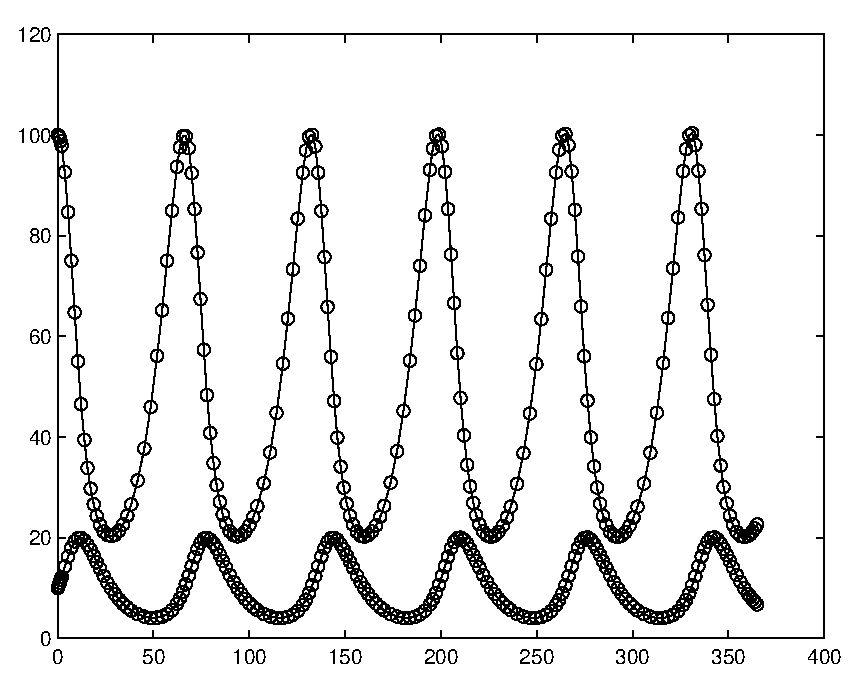
\includegraphics[height=2in]{figs/lotka.eps}}

The x-axis is time in days; the y-axis is population.  The top
curve shows the population of rabbits; the bottom curve shows
foxes.  This result is one of several patterns
this system can fall into, depending on the starting conditions
and the parameters.  As an exercise, try experimenting with
different values.


\section{What can go wrong?}

The output \index{vector} from the rate function
has to be a column \index{vector}; otherwise you get

\begin{verbatim}
Error using odearguments (line 90)
LOTKA must return a column \index{vector}.

Error in ode45 (line 115)
    odearguments(FcnHandlesUsed, solver_name, ode,...
    tspan, y0, options, varargin);
\end{verbatim}

Which is pretty good as error messages go.  It's not clear {\em why}
it needs to be a column \index{vector}, but that's not our problem.

Another possible error is reversing the order of the elements in the
initial conditions, or the \index{vector}s inside {\tt lotka}.  Again, MATLAB
doesn't know what the elements are supposed to mean, so it can't catch
errors like this; it will just produce incorrect results.


\section{Output matrices}

As we saw before, if you call {\tt ode45} without assigning the
results to variables, it plots the results.  
If you assign
the results to variables, it suppresses the figure.
Here's what that looks like:

\begin{verbatim}
>> [T, M] = ode45(@lotka, [0, 365], [100, 10]);
\end{verbatim}

You can think of the left side of this assignment as a \index{vector}
of variables.

As in previous examples, {\tt T} is a \index{vector} of time values where {\tt
ode45} made estimates.  But unlike previous examples, the
second output variable is a matrix containing one column for each
variable (in this case, $R$ and $F$) and one row for each time value.

\begin{verbatim}
>> size(M)

ans = 185     2
\end{verbatim}

This structure---one column per variable---is a common way to
use matrices.  {\tt plot} understands this structure, so if you
do this:

\begin{verbatim}
>> plot(T, M)
\end{verbatim}

MATLAB understands that it should plot each column from {\tt M}
versus {\tt T}.

You can copy the columns of {\tt M} into other variables like
this:

\begin{verbatim}
>> R = M(:, 1);
>> F = M(:, 2);
\end{verbatim}

In this context, the colon represents the range from 1 to {\tt end},
so {\tt M(:, 1)} means ``all the rows, column 1'' and
{\tt M(:, 2)} means ``all the rows, column 2.''

\begin{verbatim}
>> size(R)

ans = 185     1

>> size(F)

ans = 185     1
\end{verbatim}

So {\tt R} and {\tt F} are column \index{vector}s.  


If you plot these
\index{vector}s against each other, like this

\begin{verbatim}
>> plot(R, F)
\end{verbatim}

You get a {\bf phase plot} that looks like this:

\beforefig \centerline{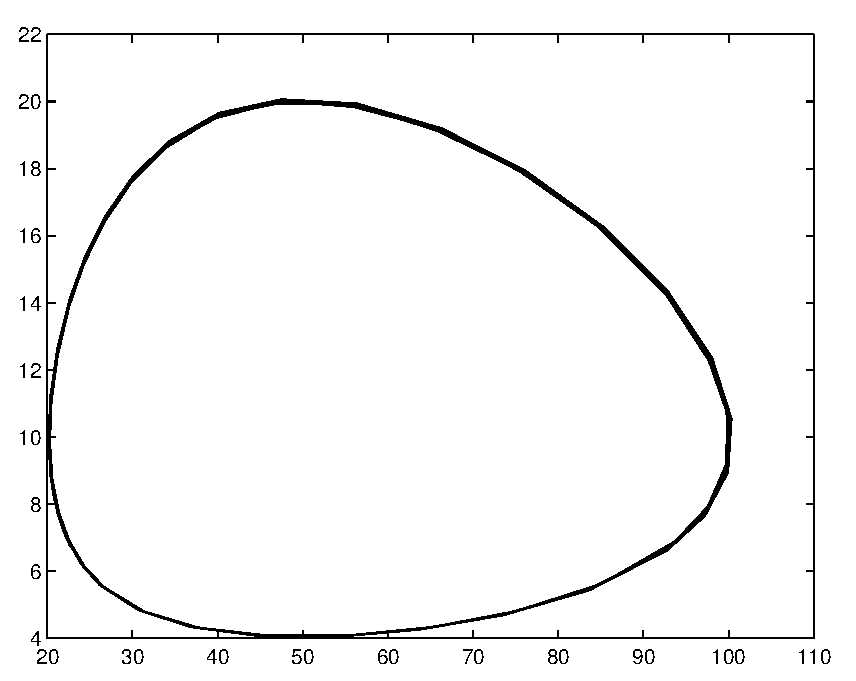
\includegraphics[height=2in]{figs/phase.eps}}

Each point on this plot represents a certain number of rabbits (on the
x axis) and a certain number of foxes (on the y axis).

Since these are the only two variables in the system, each point in
this plane describes the complete {\bf state} of the system.

Over time, the state moves around the plane; this figure shows
the path traced by the state during the time interval.  This path
is called a {\bf trajectory}.

Since the behavior of this system is periodic, the resulting
trajectory is a loop.

If there are 3 variables in the system, we need 3 dimensions to show
the state of the system, so the trajectory is a 3-D curve.
You can use {\tt plot3} to trace trajectories in 3 dimensions,
but for 4 or more variables, you are on your own.


\section{Glossary}

\begin{description}

\item[row \index{vector}:] A matrix that has only one row. 

\item[column \index{vector}:] A matrix that has only one column. 

\item[transpose:] An operation that transforms the rows of a matrix
into columns (or the other way around, if you prefer). 

\item[system of equations:] A set of equations written in terms of
a set of variables such that the equations are intertangled.

\item[paragraph:] A chunk of code that makes up part of a function,
usually with an explanatory comment. 

\item[unpack:] To copy the elements of a \index{vector} into a set of variables.

\item[pack:] To copy values from a set of variables into a \index{vector}. 

\item[state:] If a system can be described by a set of variables,
the values of those variables are called the state of the system.

\item[phase plot:] A plot that shows the state of a system as point
in the space of possible states.  

\item[trajectory:] A path in a phase plot that shows how the state of
a system changes over time.


\end{description}

\section{Exercises}

\begin{ex}

Based on the examples we have seen so far, you would think that
all ODEs describe population as
a function of time, but that's not true.

According to the
Wikipedia\footnote{\url{https://en.wikipedia.org/wiki/Lorenz_attractor}},
``The Lorenz attractor, introduced by Edward Lorenz in 1963, is a
non-linear three-dimensional deterministic dynamical system derived
from the simplified equations of convection rolls arising in the
dynamical equations of the atmosphere. For a certain set of parameters
the system exhibits chaotic behavior and displays what is today called
a strange attractor...''

The system is described by this system of differential equations:
%
\begin{eqnarray}
x_t &=& \sigma (y - x)  \\
y_t &=& x (r - z) - y   \\
z_t &=& xy - b z
\end{eqnarray}
%
Common values for the parameters are $\sigma = 10$, $b = 8/3$ and $r=28$.

Use {\tt ode45} to estimate a solution to this
system of equations.  


\begin{enumerate}

\item  The first step is to write a function named {\tt lorenz} that
takes {\tt t} and {\tt V} as input variables, where the components
of {\tt V} are understood to be the current values of {\tt x},
{\tt y} and {\tt z}.  It should compute the corresponding derivatives
and return them in a single column \index{vector}.

\item The next step is to test your function by calling it from
the command line with values like
$t=0$, $x=1$, $y=2$ and $z=3$?  Once you get your function working,
you should make it a silent function before calling {\tt ode45}.

\item Assuming that Step 2 works, you can use {\tt ode45}
to estimate the solution for the time interval $t_0 = 0$, $t_e = 30$
with the initial condition $x=1$, $y=2$ and $z=3$.

\item Use {\tt plot3} to plot the trajectory of
$x$, $y$ and $z$.

\end{enumerate}

\end{ex}


% chap10
\chapter{Second-order systems}


\section{Nested functions}

In the Section~\ref{funfiles}, we saw an example of an M-file with
more than one function:

\begin{verbatim}
function res = duck()
    error = error_func(10)
end

function res = error_func(h)
    rho = 0.3;      % density in g / cm^3
    r = 10;         % radius in cm
    res = ...
end
\end{verbatim}

Because the first function ends before the second begins, they are at
the same level of indentation.  Functions like these are {\bf
parallel}, as opposed to {\bf nested}.  A nested function is
defined inside another, like this:

\begin{verbatim}
function res = duck()
    error = error_func(10)

    function res = error_func(h)
        rho = 0.3;      % density in g / cm^3
        r = 10;         % radius in cm
        res = ...
    end
end
\end{verbatim}

The top-level function, {\tt duck}, is
the {\bf outer function} and {\tt error\_func} is
an {\bf inner function}.

Nesting functions is useful because the variables of the outer
function can be accessed from the inner function.  This is not
possible with parallel functions.

In this example, using a nested function makes it possible to
move the parameters {\tt rho} and {\tt r} out of {\tt error\_func}.

\begin{verbatim}
function res = duck(rho)
    r = 10;
    error = error_func(10)

    function res = error_func(h)
        res = ...
    end
end
\end{verbatim}

Both {\tt rho} and {\tt r} can be accessed from {\tt error\_func}.
By making {\tt rho} an input argument, we made it easier to test
{\tt duck} with different parameter values.



\section{Newtonian motion}

Newton's second law of motion is often written like this

\[ F = ma \]

where $F$ is the net force acting on a object, $m$ is the mass
of the object, and $a$ is the resulting acceleration of the object.
In a simple case where the object is moving along a straight line,
$F$ and $a$ are scalars, but in general they are \index{vector}s.

Even more generally, if $F$ and $a$ vary in time, then they can
be thought of as functions that return \index{vector}s; that is, $F$ is
a function and the result of evaluating $F(t)$ is a \index{vector} that
describes the net force at time $t$.  So a more explicit way to
write Newton's law is

\[ \forall t: \vec{F}(t) = m \vec{a}(t) \]

The arrangement of this equation suggests that if you know $m$ and $a$
you can compute force, which is true, but in most physical
simulations it is the other way around.  Based on a physical
model, you know $F$ and $m$, and compute $a$.

So if you know acceleration, $a$, as a function of time, how do you
find the position of the object, $p$?  Well, we know that acceleration
is the second derivative of position, so we can write a differential
equation


\[ \frac{d^2p}{dt^2} = a\]


Where $a$ and $p$ are functions of time that return \index{vector}s,
and $\frac{d^2p}{dt^2}$ is the second time derivative of $p$.

Because this equation includes a second derivative, it is a second-order
ODE.  {\tt ode45} can't solve this equation in this form, but by
introducing a new variable, $v$, for velocity, we can rewrite it as
a system of first-order ODEs.

\begin{eqnarray*}
\frac{dp}{dt} &=& v \\
\\
\frac{dv}{dt} &=& a
\end{eqnarray*}

The first equation says that the first derivative of $p$ is $v$; the
second says that the derivative of $v$ is $a$.


\section{Freefall}
\label{freefall}

Let's start with a simple example, an object in freefall in a vacuum
(where there's no air resistance).  Near the surface of the earth, the
acceleration of gravity is $g = -9.8$ $m/s^2$, where the minus sign
indicates that gravity pulls down.

If the object falls straight down (in the same direction as gravity),
we can describe its position with a scalar value, altitude.  So
this will be a one-dimensional problem, at least for now.

Here is a rate function we can use with {\tt ode45} to solve
this problem:

\begin{verbatim}
function res = freefall(t, X)
    p = X(1);      % the first element is position
    v = X(2);      % the second element is velocity

    dpdt = v;                          
    dvdt = acceleration(t, p, v);

    res = [dpdt; dvdt];    % pack the results in a column \index{vector}
end

function res = acceleration(t, p, v)
    g = -9.8;      % acceleration of gravity in m/s^2
    res = g;
end
\end{verbatim}

The first function is the rate function.  It gets {\tt t} and
{\tt X} as input variables, where the elements of {\tt X} are understood
to be position and velocity.  The return value from {\tt freefall}
is a (column) \index{vector} that contains the derivatives of position
and velocity, which are velocity and acceleration, respectively. 

Computing $p_t$ is easy because we are given velocity
as an element of {\tt X}.  The only thing we have to compute is
acceleration, which is what the second function does.

{\tt acceleration} computes acceleration as a function of time,
position and velocity.  In this example, the net acceleration is
a constant, so we don't really have to include all this information
yet, but we will soon.

Here's how to run {\tt ode45} with this rate function:

\begin{verbatim}
>> ode45(@freefall, [0, 30], [4000, 0])
\end{verbatim}
 
As always, the first argument is the function handle, the second
is the time interval (30 seconds) and the third is the initial
condition: in this case, the initial altitude is 4000 meters and
the initial velocity is 0.  So you can think of the ``object'' a
a skydiver jumping out of an airplane at about 12,000 feet.

Here's what the result looks like:

\beforefig \centerline{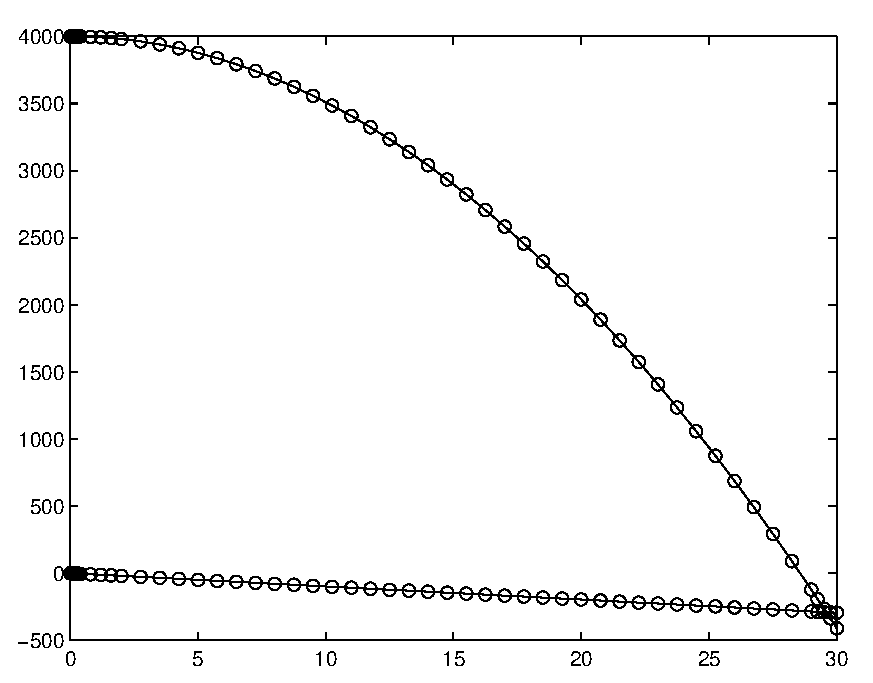
\includegraphics[height=2in]{figs/freefall.eps}}

The bottom line shows velocity starting at zero and dropping
linearly.  The top line shows position starting at 4000 m and
dropping parabolically (but remember that this parabola
is a function of time, not a ballistic trajectory).

Notice that {\tt ode45} doesn't know where the ground is, so the
skydiver keeps going through zero into negative altitude.  We will
address this issue later.


\section{Air resistance}

To make this simulation more realistic, we can add air resistance.
For large objects moving quickly through air, the force due to air
resistance, called ``drag,'' is proportional to $v^2$:

\[ F_{drag} = c v^2 \]

Where $c$ is a drag constant that depends on the density of
air, the cross-sectional area of the object and
the surface properties of the object.  For purposes of this
problem, let's say that $c = 0.2$.

To convert from force to acceleration, we have to know mass, so let's
say that the skydiver (with equipment) weighs 75 kg.

Here's a \index{version} of {\tt acceleration} that takes air resistance
into account (you don't have to make any changes in the {\tt freefall} function:

\begin{verbatim}
function res = acceleration(t, p, v)
    a_grav = -9.8;              % acceleration of gravity in m/s^2
    c = 0.2;                    % drag constant
    m = 75;                     % mass in kg
    f_drag = c * v^2;           % drag force in N
    a_drag = f_drag / m;        % drag acceleration in m/s^2
    res = a_grav + a_drag;      % total acceleration
end
\end{verbatim}

The sign of the drag force (and acceleration) is positive as
long as the object is falling, the direction of the drag force is
up.
The net
acceleration is the sum of gravity and drag.  Be careful when you
are working with forces and accelerations; make sure you only add
forces to forces or accelerations to accelerations.  In my code,
I use comments to remind myself what units the values are in.
That helps me avoid nonsense like adding forces to accelerations.

Here's what the result looks like with air resistance:

\beforefig \centerline{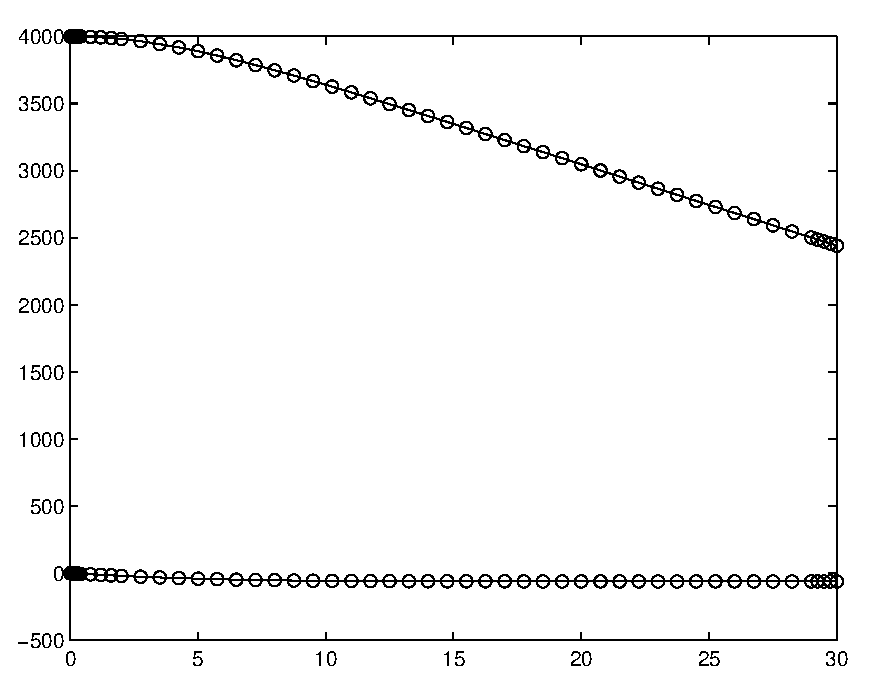
\includegraphics[height=2in]{figs/freefall2.eps}}

Big difference!  With air resistance, velocity increases until
the drag acceleration equals $g$; after that, velocity is a constant,
known as ``terminal velocity,'' and position decreases linearly
(and much more slowly than it would in a vacuum).  To examine
the results more closely, we can assign them to variables


\begin{verbatim}
>> [T, M] = ode45(@freefall, [0, 30], [4000, 0]);
\end{verbatim}

And then read the terminal position and velocity:

\begin{verbatim}
>> M(end,1)

ans = 2.4412e+03          % altitude in meters

>> M(end,2)

ans = -60.6143            % velocity in m/s
\end{verbatim}

\begin{ex}
Increase the mass of the skydiver, and confirm that
terminal velocity increases.  This relationship is the source of the
intuition that heavy objects fall faster; in air, they do!
\end{ex}


\section{Parachute!}

In the previous section, we saw that the terminal velocity of a $75
kg$ skydiver is about 60 $m/s$, which is about 130 mph.  If you hit
the ground at that speed, you would almost certainly be killed.
That's where parachutes come in.

\begin{ex}
Modify {\tt acceleration} so that after 30 seconds of
free-fall the skydiver deploys a parachute, which (almost) instantly
increases the drag constant to 2.7.

What is the terminal velocity now?  How long (after deployment) does
it take to reach the ground?
\end{ex}


\section{Two dimensions}
\label{projectile}

So far we have used {\tt ode45} for a system of first-order
equations and for a single second-order equation.  The next logical
step is a system of second-order equations, and the next logical example
is a projectile.  A ``projectile'' is an object propelled
through space, usually toward, 
and often to the detriment of,
a target.

If a projectile stays in a plane, we can think of the system as
two-dimensional, with $x$ representing the horizontal distance
traveled and $y$ representing the height or altitude.  So now
instead of a skydiver, think of a circus performer being fired
out of a cannon.

According to the
Wikipedia\footnote{\url{https://en.wikipedia.org/wiki/Human_cannonball}},
the record distance for a human cannonball is 56.5 meters (almost 186
feet).

Here is a general framework for computing the trajectory of a projectile
in two dimensions using {\tt ode45}:

\begin{verbatim}
function res = projectile(t, W)
    P = W(1:2);
    V = W(3:4);

    dPdt = V;                          
    dVdt = acceleration(t, P, V);

    res = [dPdt; dVdt];
end

function res = acceleration(t, P, V)
    g = -9.8;             % acceleration of gravity in m/s^2
    res = [0; g];
end
\end{verbatim}

The second argument of the rate function is a \index{vector}, {\tt W}, with
four elements.  The first two are assigned to {\tt P}, which
represents position; the last two are assigned to {\tt V}, which
represents velocity.
{\tt P} and {\tt V} are \index{vector}s with
elements for the $x$ and $y$ components.

The result from
{\tt acceleration} is also a \index{vector}; ignoring air resistance
(for now), the acceleration in the $x$ direction is 0; in
the $y$ direction it's $g$.
Other than that, this code is similar to what we saw in
Section~\ref{freefall}.

If we launch the human projectile from an initial height of
3 meters, with velocities 40 m/s and 30 m/s in the $x$ and $y$
directions, the {\tt ode45} call looks like
this:

\begin{verbatim}
ode45(@projectile, [0,10], [0, 3, 40, 30]);
\end{verbatim}

And the result looks like this:

\beforefig \centerline{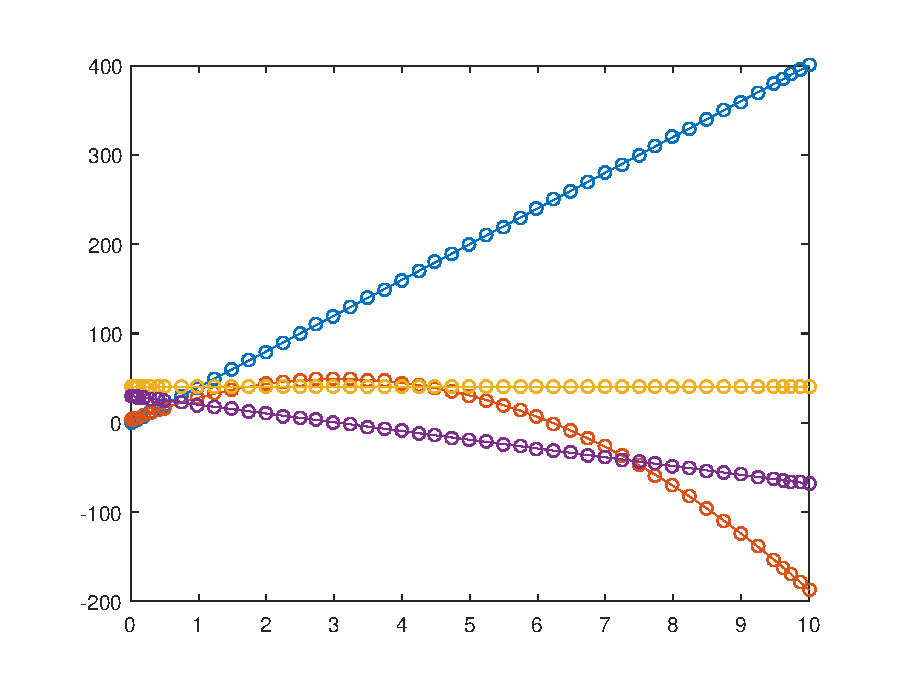
\includegraphics[height=2in]{figs/proj1_10s.eps}}

You might have to think a little to figure out which line is
which.  It looks like the flight time is about 6 seconds.

\begin{ex}
Extract the $x$ and $y$ components of
position, plot the trajectory of the projectile, and estimate the
distance traveled.
\end{ex}

\begin{ex}
Add air resistance to this simulation.  In
the skydiver scenario, we estimated that the drag constant was
$0.2$, but that was based on the assumption that the skydiver is
falling flat.  A human cannonball, flying head-first, probably
has a drag constant closer to $0.1$.  What initial velocity
is needed to achieve the record flight distance of 65.6 meters?
Hint: what is the optimal launch angle?
\end{ex}


\section{What could go wrong?}

What could go wrong?  Well, {\tt vertcat} for one.  To explain
what that means, I'll start with {\bf catenation}, which is
the operation of joining two matrices into a larger matrix.
``Vertical catenation'' joins the matrices by stacking them on
top of each other; ``horizontal catenation'' lays them
side by side.

Here's an example of horizontal catenation with row \index{vector}s:

\begin{verbatim}
>> x = 1:3

x = 1     2     3

>> y = 4:5

y = 4     5

>> z = [x, y]

z = 1     2     3     4     5
\end{verbatim}

Inside brackets, the comma operator performs horizontal catenation.
The vertical catenation operator is the semi-colon.  Here is an
example with matrices:

\begin{verbatim}
>> X = zeros(2,3)

X =  0     0     0
     0     0     0

>> Y = ones(2,3)

Y =  1     1     1
     1     1     1

>> Z = [X; Y]

Z =  0     0     0
     0     0     0
     1     1     1
     1     1     1
\end{verbatim}

These operations only work if the matrices are the same size along
the dimension where they are glued together.  If not, you get:

\begin{verbatim}
>> a = 1:3

a = 1     2     3

>> b = a'

b =  1
     2
     3

>> c = [a, b]
Error using horzcat
Dimensions of matrices being concatenated are not
consistent.

>> c = [a; b]
Error using vertcat
Dimensions of matrices being concatenated are not
consistent.

\end{verbatim}

In this example, {\tt a} is a row \index{vector} and {\tt b} is a column
\index{vector}, so they can't be catenated in either direction.

Reading the error messages, you probably guessed that {\tt horzcat}
is the function that performs horizontal catenation, and likewise
with {\tt vertcat} and vertical catenation.

These operations are relevant to {\tt projectile} because of the
last line, which packs {\tt dPdt} and {\tt dVdt} into the
output variable:

\begin{verbatim}
function res = projectile(t, W)
    P = W(1:2);
    V = W(3:4);

    dPdt = V;                          
    dVdt = acceleration(t, P, V);

    res = [dPdt; dVdt];
end
\end{verbatim}

As long as both {\tt dPdt} and {\tt dVdt} are column \index{vector}s,
the semi-colon performs vertical catenation, and the result is
a column \index{vector} with four elements.  But if either of them is a
row \index{vector}, that's trouble.

{\tt ode45} expects the result from {\tt projectile} to be a
column \index{vector}, so if you are working with {\tt ode45}, it is
probably a good idea to make {\em everything} a column \index{vector}.

In general, if you run into problems with {\tt horzcat} and {\tt
vertcat}, use {\tt size} to display the dimensions of the operands,
and make sure you are clear on which way your \index{vector}s go.


\section{Glossary}

\begin{description}

\item[parallel functions:] Two or more functions defined side-by-side,
so that one ends before the next begins.

\item[nested function:] A function defined inside another function.

\item[outer function:] A function that contains another function
definition.

\item[inner function:] A function defined inside another function
definition.  The inner function can access the variables of the
outer function.

\item[catenation:] The operation of joining two matrices end-to-end to
form a new matrix.


\end{description}

\section{Exercises}

\begin{ex}
\label{baseball}

The flight of a baseball is governed by three forces: gravity,
drag due to air resistance, and Magnus force due to spin.  If
we ignore wind and Magnus force, the path of the baseball stays
in a plane, so we can model it as a projectile in two
dimensions.

A simple model of the drag of a baseball is:
%
\[ F_d = -\frac{1}{2} ~ \rho ~ v^2 ~ A ~ C_d ~ \hat{V}   \]
%
where $F_d$ is a \index{vector} that represents the force on the baseball due
to drag, $C_d$ is the drag coefficient (0.3 is a reasonable choice),
$\rho$ is the density of air (1.3 kg/m$^3$ at sea level), $A$ is the
cross sectional area of the baseball (0.0042 m$^2$), $v$ is the
magnitude of the velocity \index{vector}, and $\hat{V}$ is a unit \index{vector} in
the direction of the velocity \index{vector}.  The mass of the baseball is
$0.145$ kg.

For more information about drag, see
\url{https://en.wikipedia.org/wiki/Drag_(physics)}.

\begin{itemize}

\item Write a function that takes the initial velocity of the baseball
and the launch angle as input variables, uses {\tt ode45} to compute
the trajectory, and returns the range (horizontal distance in flight)
as an output variable.

\item Write a function that takes the initial velocity of the baseball
as an input variable, computes the launch angle that maximizes
the range, and returns the optimal angle and range as output variables.
How does the optimal angle vary with initial velocity? Hint: To have a better 
understanding on what optimal means, you can refer to Section 11.2.

\item When the Red Sox won the World Series in 2007, they played the
Colorado Rockies at their home field in Denver, Colorado.  Find an
estimate of the density of air in the Mile High City.  What effect
does this have on drag?  Make a prediction about what effect this will
have on the optimal launch angle, and then use your simulation to test
your prediction.

\item The Green Monster in Fenway Park is about 12 m high and about 97
m from home plate along the left field line.  What is the minimum
speed a ball must leave the bat in order to clear the monster
(assuming it goes off at the optimal angle)?  Do you think it is
possible for a person to stand on home plate and throw a
ball over the Green Monster?

\item The actual drag on a baseball is more complicated than what is
captured by our simple model.  In particular, the drag coefficient
varies with velocity.  You can get some of the details from {\em The
Physics of Baseball}\footnote{Robert K. Adair, Harper Paperbacks, 3rd
Edition, 2002.}; you also might find information on the web.
Either way, specify a more realistic model of drag and modify your
program to implement it.  How big is the effect on your computed
ranges?  How big is the effect on the optimal angles?

\end{itemize}

\end{ex}


% chap11
\chapter{Optimization and Interpolation}

\section{ODE Events}
\label{events}

Normally when you call {\tt ode45} you have to specify
a start time and an end time.  But in many cases, you don't know ahead
of time when the simulation should end.
Fortunately MATLAB provides a mechanism for dealing
with this problem.  The bad news is that it is a little awkward.
Here's how it works:

\begin{enumerate}

\item Before calling {\tt ode45} you use {\tt odeset} to create an
object called {\tt options} that contains values that control
how {\tt ode45} works:

\begin{verbatim}
options = odeset('Events', @events);
\end{verbatim}
%
In this case, the name of the option is {\tt Events} and the
value is a function handle.  When {\tt ode45} runs, it will invoke
{\tt events} after each timestep.
You can call this function anything you want, but the name
{\tt events} is conventional.

\item The function you provide has to take
the same input variables as your rate function.  For example,
here is an event function that would work with {\tt projectile}
from Section~\ref{projectile}

\begin{verbatim}
function [value,isterminal,direction] = events(t,X)
    value = X(2);        % Extract the current height.
    isterminal = 1;      % Stop the integration if height crosses zero.
    direction = -1;      % But only if the height is decreasing.
end
\end{verbatim}

{\tt events} returns three output variables:

{\tt value} determines
when an event occurs.  In this case {\tt value} gets the second
element of {\tt X}, which is understood to be the height of the
projectile.  An ``event'' is a point in time when this value passes
through 0.

{\tt direction} determines whether an event occurs when
{\tt value} is increasing ({\tt direction=1}), decreasing ({\tt
direction=-1}, or both {\tt direction=0}.

{\tt isterminal} determines what happens when an event
occurs.  If {\tt isterminal=1}, the event is ``terminal'' and the
simulation stops.  If {\tt isterminal=0}, the simulation continues,
but {\tt ode45} does some additional work to make sure that the
solution in the vicinity of the event is accurate, and that one of the
estimated values in the result is at the time of the event.

\item When you call {\tt ode45}, you pass {\tt options} as a fourth
argument:

\begin{verbatim}
ode45(@projectile, [0,10], [0, 3, 40, 30], options);
\end{verbatim}
%
\end{enumerate}

\begin{ex}
How would you modify {\tt events} to stop when the height of
the projectile falls through 3m?
\end{ex}


\section{Optimization}

In Exercise~\ref{baseball}, you were asked to find the optimal
launch angle for a batted ball.  ``Optimal'' is a fancy way of
saying ``best;'' what that means depends on the problem.  For
the Green Monster Problem---finding the optimal angle for
hitting a home run in Fenway Park, the meaning of ``optimal''
is not obvious.

It is tempting to choose the angle that yields the longest
range (distance from home plate when it lands).  But in this
case we are trying to clear a 12m wall, so maybe we want
the angle that yields the longest range when the ball falls
through 12m.

Although either definition would be good enough for most purposes,
neither is quite right.  In this case the ``optimal'' angle is
the one that yields the greatest height at the point where
the ball reaches the wall, which is 97m from home plate.

So the first step in any optimization problem is to define
what ``optimal'' means.  The second step is to define a range of
values where you want to search.  In this case the range of
feasible values is between 0 degrees (parallel to the ground)
and 90 degrees (straight up).  We expect the
optimal angle to be near 45 degrees, but we might not be sure
how far from 45 degrees to look.  To play it safe, we could
start with the widest feasible range.

The simplest way to search for an optimal value is to run the
simulation with a wide range of values and choose the one
that yields the best result.  This
method is not very efficient, especially in a case like this where
computing the distance in flight is expensive.

A better algorithm is a Golden Section Search.  

\section{Golden section search}

To present the Golden Section Search, I will start with a simplified
\index{version} I'll call a Silver Section Search.  The basic idea is similar to
the methods for zero-finding we saw in Section~\ref{zero}.  In the
case of zero-finding, we had a picture like this:

\beforefig \centerline{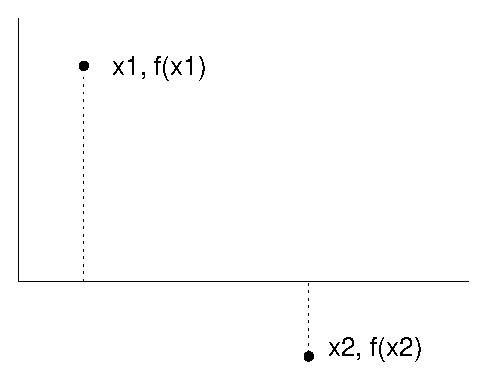
\includegraphics[height=1.5in]{figs/secant.eps}}

We are given a function, $f$, that we can evaluate, and
we want to find a root of $f$; that is, a value of $x$ that makes
$f(x)=0$.  If we can find a value, $x_1$, that makes $f(x_1)$ positive
and another value, $x_2$, that makes $f(x_2)$ negative, then there has
to be a root in between (as long as $f$ is continuous).  In this
case we say that $x_1$ and $x_2$ ``bracket'' the root.

The algorithm proceeds by choosing a third value, $x_3$, between
$x_1$ and $x_2$ and then evaluating $y = f(x_3)$.  If $y$ is
positive, we can form a new pair, $(x_3, x_2)$, that brackets the
root.  If $y$ is negative then the pair $(x_1, x_3)$ brackets the root.
Either way the size of the bracket gets smaller, so our
estimate of the location of the root gets better.

So that was root-finding.  The Sliver Section Search is similar, but
we have to start with three values, and the picture looks like
this:

\beforefig \centerline{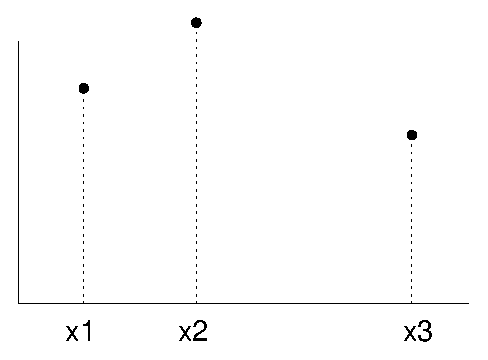
\includegraphics[height=1.5in]{figs/golden1.eps}}

This diagram shows that we have evaluated $f$ in three places,
$x_1$, $x_2$ and $x_3$, and found that $x_2$ yields the highest
value.  If $f$ is continuous, then there has to be at least one
local maximum between $x_1$ and $x_3$, so we would say that the
triple $(x_1, x_2, x_3)$ brackets a maximum.

The next step is to choose a fourth point, $x_4$, and evaluate
$f(x_4)$.  There are two possible outcomes, depending on whether
$f(x_4)$ is greater than $f(x_2)$:

\beforefig \centerline{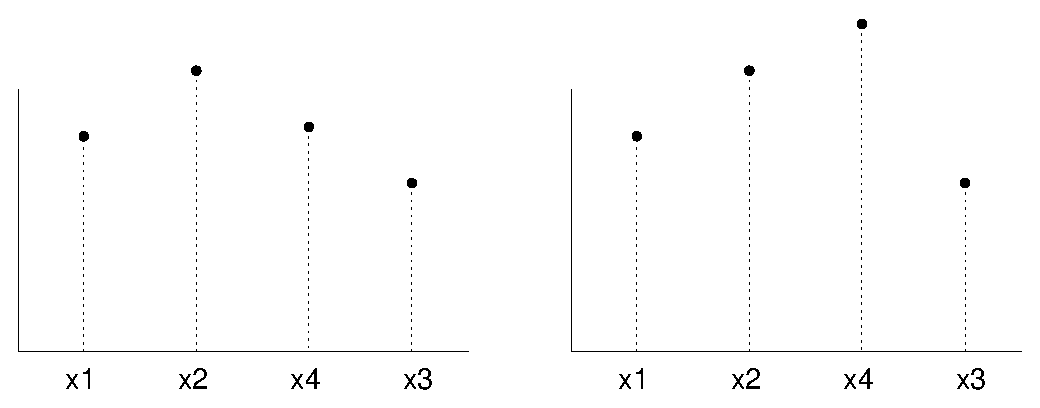
\includegraphics[height=1.5in]{figs/golden2.eps}}

If $f(x_4)$ is less than than $f(x_2)$ (shown on the left), then the
new triple $(x_1, x_2, x_4)$ brackets the maximum.  If $f(x_4)$ is
greater than $f(x_2)$ (shown on the right), then $(x_2, x_4, x_3)$
brackets the maximum.  Either way the range gets smaller and our
estimate of the optimal value of $x$ gets better.

This method works for almost any value of $x_4$, but some choices
are better than others.  In the example, I chose to bisect the
bigger of the ranges $(x_1, x_2)$ and $(x_2, x_3)$.

Here's what that looks like in MATLAB:

\begin{verbatim}
function res = optimize(V)
    x1 = V(1);
    x2 = V(2);
    x3 = V(3);
    
    fx1 = height_func(x1);
    fx2 = height_func(x2);
    fx3 = height_func(x3);
   
    for i=1:50
        if x3-x2 > x2-x1
            x4 = (x2+x3) / 2;
            fx4 = height_func(x4);
            if fx4 > fx2
                x1 = x2;  fx1 = fx2;
                x2 = x4;  fx2 = fx4;
            else
                x3 = x4;  fx3 = fx4;
            end
        else
            x4 = (x1+x2) / 2;
            fx4 = height_func(x4);
            if fx4 > fx2
                x3 = x2;  fx3 = fx2;
                x2 = x4;  fx2 = fx4;
            else
                x1 = x4;  fx1 = fx4;
            end
        end

        if abs(x3-x1) < 1e-2
            break
        end
    end
    res = [x1 x2 x3];
end
\end{verbatim}

The input variable is a \index{vector} that contains three values that bracket
a maximum; in this case they are angles in degrees.  {\tt optimize}
starts by evaluating {\tt height\_func} for each of the three values.
We assume that {\tt height\_func} returns the quantity we want to
optimize; for the Green Monster Problem it is the height of
the ball when it reaches the wall.

Each time through the {\tt for} loop the function chooses a value
of {\tt x4}, evaluates {\tt height\_func}, and then updates the
triplet {\tt x1}, {\tt x2} and {\tt x3} according to the results.

After the update, it computes the range of the bracket, {\tt x3-x1},
and checks whether it is small enough.  If so, it breaks out of
the loop and returns the current triplet as a result.  In the
worst case the loop executes 50 times.

\begin{ex}
I call this algorithm a Silver Section Search because it is almost as
good as a Golden Section Search.  Read the Wikipedia page about the
Golden Section Search
(\url{https://en.wikipedia.org/wiki/Golden_section_search}) and then
modify this code to implement it.
\end{ex}

\begin{ex}
You can write functions that take function handles as input
variables, just as {\tt fzero} and {\tt ode45} do.
For example, {\tt handle\_func} takes a function handle called
{\tt func} and calls it, passing {\tt pi} as an argument.

\begin{verbatim}
function res = handle_func(func)
    func(pi)
end
\end{verbatim}

You can call {\tt handle\_func} from the Command Window and pass
different function handles as arguments:

\begin{verbatim}
>> handle_func(@sin)

ans = 0

>> handle_func(@cos)

ans = -1
\end{verbatim}

Modify {\tt optimize} so that it takes a function handle
as an input variable and uses it as the function to be
optimized.
\end{ex}

\begin{ex}
The MATLAB function {\tt fminsearch} takes a function handle
and searches for a local minimum.  Read the documentation for
{\tt fminsearch} and use it to find the optimal launch angle
of a baseball with a given velocity.
\end{ex}


\section{Discrete and continuous maps}

When you solve an ODE analytically, the result is a function,
which you can think of as a continuous map.  When you use an
ODE solver, you get two \index{vector}s (or a \index{vector} and a matrix), which
you can think of as a discrete map.

For example, in Section~\ref{ode45}, we used the following rate
function to estimate the population of rats as a function of time:

\begin{verbatim}
function res = rats(t, y)
    a = 0.01;
    omega = 2 * pi / 365;
    res = a * y * (1 + sin(omega * t));
end
\end{verbatim}

The result from {\tt ode45} is two \index{vector}s:

\begin{verbatim}
>> [T, Y] = ode45(@rats, [0, 365], 2);
\end{verbatim}

{\tt T} contains the time values where {\tt ode45} estimated the
population; {\tt Y} contains the population estimates.

Now suppose we would like to know the population on the 180th day
of the year.  We could search {\tt T} for the value 180:

\begin{verbatim}
>> find(T==180)

ans = Empty matrix: 0-by-1
\end{verbatim}

But there is no guarantee that any particular value appears in
{\tt T}.  We can find the index where {\tt T} crosses 180:

\begin{verbatim}
>> I = find(T>180); I(1)

ans = 23
\end{verbatim}

{\tt I} gets the indices of all elements of {\tt T} greater
than 180, so {\tt I(1)} is the index of the {\em first} one.

Then we find the corresponding value from {\tt Y}:

\begin{verbatim}
>> [T(23), Y(23)]

ans = 184.3451   40.3742
\end{verbatim}

That gives us a coarse estimate of the population on Day 180.
If we wanted to do a little better, we could also find the last value
before Day 180:

\begin{verbatim}
>> [T(22), Y(22)]

ans = 175.2201   36.6973
\end{verbatim}

So the population on Day 180 was between 36.6973 and 40.3742.

But where in this range is the best estimate?  A simple option is to
choose whichever time value is closer to 180 and use the corresponding
population estimate.  In the example, that's not a great choice
because the time value we want is right in the middle.


\section{Interpolation}

A better option is to draw a straight line between the two points that
bracket Day 180 and use the line to estimate the value in between.
This process is called {\bf linear interpolation}, and MATLAB provides
a function named {\tt interp1} that does it:

\begin{verbatim}
>> pop = interp1(T, Y, 180)

pop = 38.6233
\end{verbatim}

The first two arguments specify a discrete map from the values in
{\tt T} to the values in {\tt Y}.  The third argument is the
time value where we want to interpolate.  The result is what
we expected, about halfway between the values that bracket it.

{\tt interp1} can also take a fourth argument that specifies what
kind of interpolation you want.  The default is {\tt 'linear'}, which
does linear interpolation.  Other choices include {\tt 'spline'}
which uses a spline curve to fit two points on either side,
and {\tt 'cubic'}, which uses piecewise cubic Hermite interpolation.

\begin{verbatim}
>> pop = interp1(T, Y, 180, 'spline')

pop = 38.6486

>> pop = interp1(T, Y, 180, 'cubic')

pop = 38.6491
\end{verbatim}

In this case we expect the spline and cubic interpolations to be
better than linear, because they use more of the data, and we know the
function isn't linear.  But we have no reason to expect the spline to
be more accurate than the cubic, or the other way around.
Fortunately, they are not very different.

We can also use {\tt interp1} to project the rat population out
beyond the values in {\tt T}:

\begin{verbatim}
>> [T(end), Y(end)]

ans = 365.0000   76.9530

>> pop = interp1(T, Y, 370, 'cubic')

pop = 80.9971
\end{verbatim}

This process is called {\bf extrapolation}.  For time values near
365, extrapolation may be reasonable, but as we go farther into
the ``future,'' we expect them to be less accurate.
For example, here is the estimate we get by extrapolating for a whole
year:

\begin{verbatim}
>> pop = interp1(T, Y, 365*2, 'cubic')

pop = -4.8879e+03
\end{verbatim}

And that's wrong.  So very wrong.


\section{Interpolating the inverse function}

We have used {\tt interp1} to find population as a function of time;
by reversing the roles of {\tt T} and {\tt Y}, we can also interpolate
time as a function of population.  For example, we might want to know
how long it takes the population to reach 20.

\begin{verbatim}
>> interp1(Y, T, 20)

ans = 133.4128
\end{verbatim}

This use of {\tt interp1} might be confusing if you think of the
arguments as $x$ and $y$.  You might find it helpful to think of them
as the range and domain of a map (where the third argument is
an element of the range).

The following plot shows $f$ ({\tt Y} plotted as a function of {\tt T})
and the inverse of $f$ ({\tt T} plotted as a function of {\tt Y}).

\beforefig
\centerline{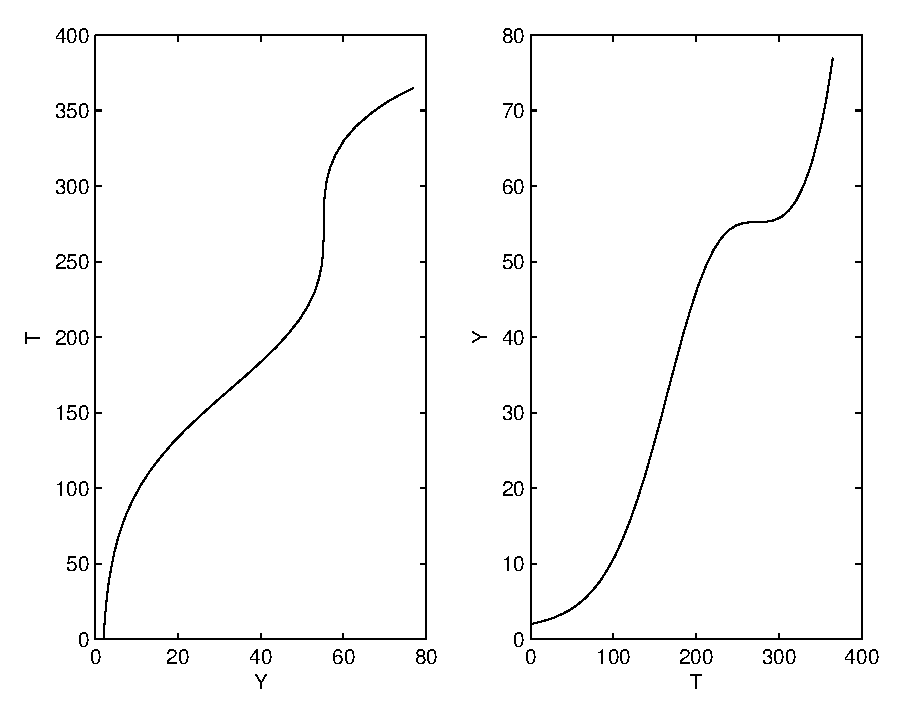
\includegraphics[height=2.2in,width=4.6in]{figs/ratplot.eps}}

In this case we can use {\tt interp1} either way because $f$ is
a {\bf single-valued mapping}, which means that for each value in
the domain, there is only one value in the range that maps to it.

If we reduce the food supply so that the rat population decreases
during the winter, we might see something like this:

\beforefig 
\centerline{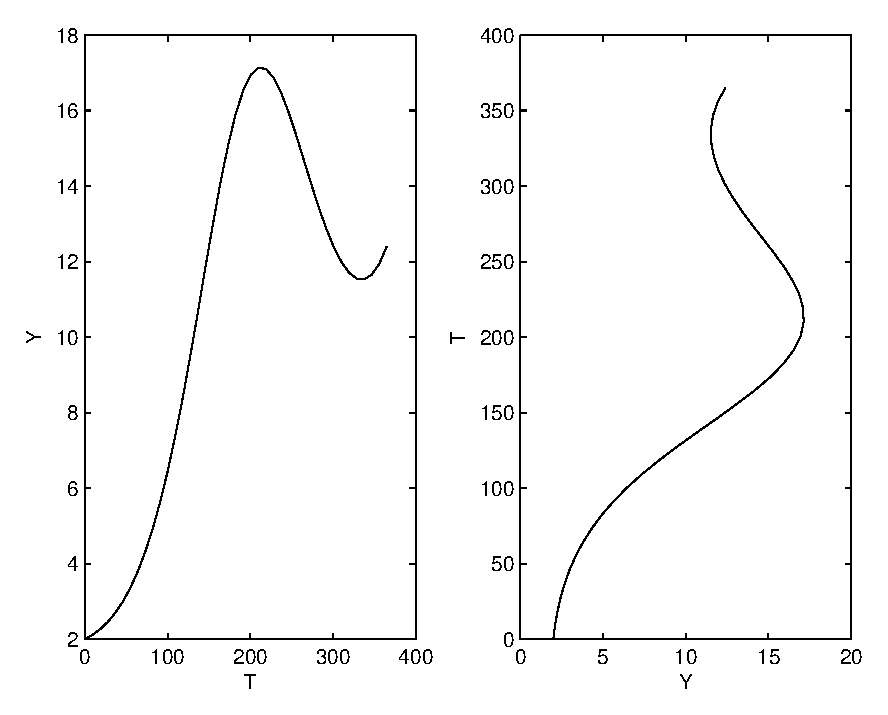
\includegraphics[height=2in,width=4in]{figs/ratplot2.eps}}

We can still use {\tt interp1} to map from {\tt T} to {\tt Y}:

\begin{verbatim}
>> interp1(T, Y, 260)

ans = 15.0309
\end{verbatim}

So on Day 260, the population is about 15, but if we ask on what
day the population was 15, there are two possible answers, 172.44
and 260.44.  If we try to use {\tt interp1}, we get the wrong answer:

\begin{verbatim}
>> interp1(Y, T, 15)         

ans = 196.3833                % WRONG
\end{verbatim}

On Day 196, the population is actually 16.8, so {\tt interp1} isn't
even close!  The problem is that {\tt T} as a function of {\tt Y} is a
{\bf multivalued mapping}; for some values in the range there are more
than one values in the domain.  This causes {\tt interp1} to fail.  


\section{Field mice}

As we've seen, one use of interpolation is to interpret the results
of a numerical computation; another is to fill in the gaps between
discrete measurements.

For example\footnote{This example is adapted from Gerald and Wheatley,
{\em Applied Numerical Analysis}, Fourth Edition, Addison-Wesley,
1989.}, suppose that the population of field mice is governed by this
rate equation:

\[ g(t, y) = ay - b(t) y^{1.7} \]

where $t$ is time in months, $y$ is population, $a$ is a parameter
that characterizes population growth in the absence of limitations,
and $b$ is a function of time that characterizes the effect of the
food supply on the death rate.

Although $b$ appears in the equation as a continuous function, we
might not know $b(t)$ for all $t$.  Instead, we might only have discrete
measurements:

\begin{verbatim}
t          b(t)
-          ----
0          0.0070
1          0.0036             
2          0.0011
3          0.0001
4          0.0004
5          0.0013
6          0.0028
7          0.0043
8          0.0056
\end{verbatim}

If we use {\tt ode45} to solve the differential equation, then we
don't get to choose the values of $t$ where the rate function
(and therefore $b$) gets evaluated.  We need to provide a function
that can evaluate $b$ everywhere:

\begin{verbatim}
function res = interpolate_b(t)
    T = 0:8;
    B = [70 36 11 1 4 13 28 43 56] * 1e-4;
    res = interp1(T, B, t);
end
\end{verbatim}

Abstractly, this function uses a discrete map to implement a
continuous map.  

\begin{ex}
Write a rate function that uses
{\tt interpolate\_b} to evaluate $g$ and then
use {\tt ode45} to compute the population of field mice
from $t=0$ to $t=8$ with an initial population of 100 and
$a=0.9$.

Then modify {\tt interpolate\_b} to use spline interpolation
and run {\tt ode45} again to see how much effect the interpolation
has on the results.
\end{ex}

\section{Glossary}

\begin{description}

\item[interpolation:] Estimating the value of a function using
known values on either side.

\item[extrapolation:] Estimating the value of a function using
known values that don't bracket the desired value.

\item[single-valued mapping:] A mapping where each value in the
range maps to a single value in the domain.

\item[multivalued mapping:] A mapping where at least one value in
the range maps to more than one value in the domain.

\end{description}


\section{Exercises}

\begin{ex}
\label{golf}

A golf ball\footnote{See
\url{https://en.wikipedia.org/wiki/Golf_ball}.} hit with backspin
generates lift, which might increase the range, but the energy that
goes into generating spin probably comes at the cost of lower initial
velocity.  Write a simulation of the flight of a golf ball and use it
to find the launch angle and allocation of spin and initial velocity
(for a fixed energy budget) that maximizes the horizontal range of the
ball in the air.

The lift of a spinning ball is due to the Magnus force\footnote{See
\url{https://en.wikipedia.org/wiki/Magnus_effect}.}, which is
perpendicular to the axis of spin and the path of flight.  The
coefficient of lift is proportional to the spin rate; for a ball
spinning at 3000 rpm it is about 0.1.  The coefficient of drag of a
golf ball is about 0.2 as long as the ball is moving faster than 20 m/s.
\end{ex}



%chap12
\chapter{\index{vector}s as \index{vector}s}

\section{What's a \index{vector}?}

The word ``\index{vector}'' means different things to different people.
In MATLAB, a \index{vector} is a matrix that has either one row or one
column.  So far we have used MATLAB \index{vector}s to represent

\begin{description}

\item[sequences:] A sequence is a set of values identified by
integer indices; it is natural to store the elements of the
sequence as elements of a MATLAB \index{vector}.

\item[state \index{vector}s:] A state \index{vector} is a set of values that
describes the state of a physical system.  When you call
{\tt ode45}, you give it in the initial conditions in a state
\index{vector}.  Then when {\tt ode45} calls your rate function, it
gives you a state \index{vector}.

\item[discrete maps:] If you have two \index{vector}s with the same
length, you can think of them as a mapping from the elements
of one \index{vector} to the corresponding elements of the other.  For
example, in Section~\ref{rats}, the results from {\tt ode45}
are \index{vector}s, {\tt T} and {\tt Y}, that represent a mapping
from the time values in {\tt T} to the population values in {\tt Y}.

\end{description}

In this chapter we will see another use of MATLAB \index{vector}s:
representing spatial \index{vector}s.  A spatial \index{vector} is a value that
represents a multidimensional physical quantity like position,
velocity, acceleration or force \footnote{See
\url{https://en.wikipedia.org/wiki/\index{vector}_(spatial)}.}.

These quantities cannot be described with a
single number because they contain multiple components.  For example,
in a 3-dimensional Cartesian coordinate space, it takes three numbers
to specify a position in space; they are usually called $x$, $y$ and
$z$ coordinates.  As another example, in 2-dimensional polar
coordinates, you can specify a velocity with two numbers, a
magnitude and an angle, often called $r$ and $\theta$.

It is convenient to represent spatial \index{vector}s using MATLAB \index{vector}s
because MATLAB knows how to perform most of the \index{vector}
operations you need for physical modeling.  For example,
suppose that you are given the velocity of a baseball in
the form of a MATLAB \index{vector} with two elements, $v_x$ and $v_y$,
which are the components of velocity in the $x$ and $y$ directions.

\begin{verbatim}
>> V = [30; 40]        % velocity in m/s
\end{verbatim}

And suppose you are asked to compute the total acceleration of
the ball due to drag and gravity.  In math notation, the force
due to drag is

\[ F_d = -\frac{1}{2} ~ \rho ~ v^2 ~ A ~ C_d ~ \hat{V}   \]

where $V$ is a spatial \index{vector} representing velocity, $v$ is the magnitude
of the velocity (sometimes called ``speed''), and $\hat{V}$ is a unit
\index{vector} in the direction of the velocity \index{vector}.  The other terms,
$\rho$, $A$ and $C_d$, are scalars.

The magnitude of a \index{vector} is the square root of the sum of the squares
of the elements.  You could compute it with {\tt hypotenuse} from
Section~\ref{hypotenuse}, or you could use the MATLAB function {\tt
norm} ({\bf norm} is another name\footnote{Magnitude is also called
``length'' but I will avoid that term because it gets confused with
the {\tt length} function, which returns the number of elements in a
MATLAB \index{vector}.}  for the magnitude of a \index{vector}):

\begin{verbatim}
>> v = norm(V)

v = 50
\end{verbatim}

$\hat{V}$ is a {\bf unit \index{vector}}, which means it should have norm 1,
and it should point in the same direction as $V$.  The simplest
way to compute it is to divide $V$ by its own norm.

\begin{verbatim}
>> Vhat = V / v

aVhat =  0.6  0.8
\end{verbatim}

Then we can confirm that the norm of $\hat{V}$ is 1:

\begin{verbatim}
>> norm(Vhat)

ans = 1
\end{verbatim}

To compute $F_d$ we just multiply the scalar terms by $\hat{V}$.

\begin{verbatim}
Fd = - 1/2 * C * rho * A * v^2 * Vhat
\end{verbatim}

Similarly, we can compute acceleration by dividing the \index{vector}
$F_d$ by the scalar $m$.

\begin{verbatim}
Ad = Fd / m
\end{verbatim}

To represent the acceleration of gravity, we create a \index{vector} 
with two components:

\begin{verbatim}
Ag = [0; -9.8]
\end{verbatim}

The $x$ component of gravity is 0; the $y$ component is $-9.8 m/s^2$.

Finally we compute total acceleration by adding \index{vector}
quantities:

\begin{verbatim}
A = Ag + Ad;
\end{verbatim}

One nice thing about this computation is that we didn't have to
think much about the components of the \index{vector}s.  By treating
spatial \index{vector}s as basic quantities, we can express complicated computations
concisely.


\section{Dot and cross products}

Multiplying a \index{vector} by a scalar is a straightforward operation;
so is adding two \index{vector}s.  But multiplying two \index{vector}s is more
subtle.  It turns out that there are two \index{vector} operations that
resemble multiplication: {\bf dot product}
and {\bf cross product}.

The dot product of \index{vector}s $A$ and $B$ is a scalar:

\[ d = a b \cos \theta \]
%
where $a$ is the magnitude of $A$, $b$ is the magnitude of $B$,
and $\theta$ is the angle between the \index{vector}s.  We already know
how to compute magnitudes, and you could probably figure out
how to compute $\theta$, but you don't have to.  MATLAB provides
a function, {\tt dot}, that computes dot products.

\begin{verbatim}
d = dot(A, B)
\end{verbatim}

{\tt dot} works in any number of dimensions, as long as {\tt A}
and {\tt B} have the same number of elements.

If one of the operands is a unit \index{vector}, you can use the dot
product to compute the component of a \index{vector} $A$ that is in
the direction of a unit \index{vector}, $\hat{i}$:

\begin{verbatim}
s = dot(A, ihat)
\end{verbatim}

In this example, $s$ is the {\bf scalar projection} of $A$
onto $\hat{i}$.  The {\bf \index{vector} projection} is the \index{vector}
that has magnitude $s$ in the direction of $\hat{i}$:

\begin{verbatim}
V = dot(A, ihat) * ihat
\end{verbatim}

The cross product of \index{vector}s $A$ and $B$ is a \index{vector} whose direction
is perpendicular to $A$ and $B$ and whose magnitude is

\[ c = a b \sin \theta \]
%
where (again) $a$ is the magnitude of $A$, $b$ is the magnitude of
$B$, and $\theta$ is the angle between the \index{vector}s.  MATLAB provides
a function, {\tt cross}, that computes cross products.

\begin{verbatim}
C = cross(A, B)
\end{verbatim}

{\tt cross} calculates the cross product of corresponding \index{vector}s along the first array dimension whose size equals 3.

A common use of {\tt cross} is to compute torques.  If you represent
a moment arm $R$ and a force $F$ as 3-dimensional \index{vector}s, then
the torque is just

\begin{verbatim}
Tau = cross(R, F)
\end{verbatim}

If the components of {\tt R} are in meters and the components
of {\tt F} are in Newtons, then the torques in {\tt Tau} are
in Newton-meters.



\section{Celestial mechanics}

Modeling celestial mechanics is a good opportunity
to compute with spatial \index{vector}s.
Imagine a star with mass $m_1$ at a point in space described by the
\index{vector} $P_1$, and a planet with mass $m_2$ at point $P_2$.  The
magnitude of the gravitational force\footnote{See
\url{https://en.wikipedia.org/wiki/Gravity}} between them is

\[ f_g = G \frac{m_1 m_2}{r^2}  \]
%
where $r$ is the distance between them and $G$ is the universal
gravitational constant, which is about $6.67 \times 10^{-11} N m^2 /
kg^2$.  Remember that this is the appropriate value of $G$ only if the
masses are in kilograms, distances in meters, and forces in Newtons.

The direction of the force on the star at $P_1$ is in the
direction toward $P_2$.  We can compute relative direction by
subtracting \index{vector}s; if we compute {\tt R = P2 - P1}, then
the direction of {\tt R} is from {\tt P1} to {\tt P2}.

The distance between the planet and star is the length of $R$:

\begin{verbatim}
r = norm(R)
\end{verbatim}

The direction of the force on the star is $\hat{R}$:

\begin{verbatim}
rhat = R / r
\end{verbatim}

\begin{ex}
Write a sequence of MATLAB statements that computes {\tt F12}, a \index{vector}
that represents the force on the star due to the planet, and {\tt
F21}, the force on the planet due to the star.
\end{ex}

\begin{ex}
Encapsulate these statements in a function named {\tt
gravity\_force\_func} that takes {\tt P1}, {\tt m1}, {\tt P2}, and
{\tt m2} as input variables and returns {\tt F12}.
\end{ex}

\begin{ex}
\label{jupiter}
Write a simulation of the orbit of Jupiter around the Sun.  The mass
of the Sun is about $2.0 \times 10^{30}$ kg.  You can get the mass of
Jupiter, its distance from the Sun and orbital velocity from
\url{https://en.wikipedia.org/wiki/Jupiter}.  Confirm that it takes
about 4332 days for Jupiter to orbit the Sun.
\end{ex}

\section{Animation}

Animation is a useful tool for checking the results of a physical
model.  If something is wrong, animation can make it obvious.
There are two ways to do animation in MATLAB.  One is to use
{\tt getframe} to capture a series of images and {\tt movie} to
play them back.
The more informal way is to draw a series of plots.
Here is an example I wrote for Exercise~\ref{jupiter}:

\begin{verbatim}
function animate_func(T,M)
    % animate the positions of the planets, assuming that the
    % columns of M are x1, y1, x2, y2.
    X1 = M(:,1);
    Y1 = M(:,2);
    X2 = M(:,3);
    Y2 = M(:,4);

    minmax = [min([X1;X2]), max([X1;X2]), min([Y1;Y2]), max([Y1;Y2])];

    for i=1:length(T)
        clf;
        axis(minmax);
        hold on;
        draw_func(X1(i), Y1(i), X2(i), Y2(i));
        drawnow;
    end
end
\end{verbatim}

The input variables are the output from {\tt ode45}, a \index{vector}
{\tt T} and a matrix {\tt M}.  The columns of {\tt M} are the
positions and velocities of the Sun and Jupiter, so
{\tt X1} and {\tt Y1} get the coordinates of the Sun;
{\tt X2} and {\tt Y2} get the coordinates of Jupiter.

{\tt minmax} is a \index{vector} of four elements which is used inside
the loop to set the axes of the figure.  This is necessary because
otherwise MATLAB scales the figure each time through the loop,
so the axes keep changing, which makes the animation hard
to watch.

Each time through the loop, {\tt animate\_func} uses {\tt clf}
to clear the figure and {\tt axis} to reset the axes.  {\tt hold
on} makes it possible to put more than one plot onto the same
axes (otherwise MATLAB clears the figure each time you call
{\tt plot}).

Each time through the loop, we have to call {\tt drawnow} so
that MATLAB actually displays each plot.  Otherwise it waits
until you finish drawing all the figures and {\em then} updates
the display.

{\tt draw\_func} is the function that actually makes the
plot:

\begin{verbatim}
function draw_func(x1, y1, x2, y2)
    plot(x1, y1, 'r.', 'MarkerSize', 50);
    plot(x2, y2, 'b.', 'MarkerSize', 20);
end
\end{verbatim}

The input variables are the position of the Sun and Jupiter.
{\tt draw\_func} uses {\tt plot} to draw
the Sun as a large red marker and Jupiter as a smaller blue one.

\begin{ex}
To make sure you understand how {\tt animate\_func} works,
try commenting out some of the lines to see what happens.
\end{ex}

One limitation of this kind of animation is that the speed
of the animation depends on how fast your computer can generate
the plots.  Since the results from {\tt ode45} are usually not
equally spaced in time, your animation might slow down where
{\tt ode45} takes small time steps and speed up where the time
step is larger.

There are two ways to fix this problem:

\begin{enumerate}

\item When you call {\tt ode45} you can give it a \index{vector} of
points in time where it should generate estimates.  Here is
an example:

\begin{verbatim}
end_time = 1000;
step = end_time/200;
[T, M] = ode45(@rate_func, [0:step:end_time], W);
\end{verbatim}

The second argument is a range \index{vector} that goes from 0 to 1000 with a
step size determined by {\tt step}.  Since {\tt step} is {\tt
end\_time/200}, there will be about 200 rows in {\tt T} and {\tt M}
(201 to be precise).

This option does not affect the accuracy of the results; {\tt ode45}
still uses variable time steps to generate the estimates, but then it
interpolates them before returning the results.

\item You can use {\tt pause} to play the animation in
real time.  After drawing each frame and calling
{\tt drawnow}, you can compute the time
until the next frame and use {\tt pause} to wait:

\begin{verbatim}
dt = T(i+1) - T(i);
pause(dt);
\end{verbatim}

A limitation of this method is that it ignores the time required to
draw the figure, so it tends to run slow, especially if the figure is
complex or the time step is small.

\end{enumerate}

\begin{ex}
Use {\tt animate\_func} and {\tt draw\_func} to vizualize your
simulation of Jupiter.  Modify it so it shows one day of simulated
time in 0.001 seconds of real time---one revolution should take
about 4.3 seconds.
\end{ex}


\section{Conservation of Energy}

A useful way to check the accuracy of an ODE solver is to
see whether it conserves energy.  For planetary
motion, it turns out that {\tt ode45} does not.

The kinetic energy of a moving body is $m v^2 / 2$; the
kinetic energy of a solar system is the total kinetic
energy of the planets and sun.
The potential energy of a sun with mass $m_1$ and a
planet with mass $m_2$ and a distance $r$ between them is

\[ U = -G \frac{m_1 m_2}{r}  \]
%

\begin{ex}
Write a function called {\tt energy\_func} that takes the output of
your Jupiter simulation, {\tt T} and {\tt M}, and computes the total
energy (kinetic and potential) of the system for each estimated
position and velocity.  Plot the result as a function of time and
confirm that it decreases over the course of the simulation.  Your
function should also compute the relative change in energy, the
difference between the energy at the beginning and end, as a
percentage of the starting energy.
\end{ex}

You can reduce the rate of energy loss by decreasing {\tt ode45}'s
tolerance option using {\tt odeset} (see Section~\ref{events}):

\begin{verbatim}
options = odeset('RelTol', 1e-5);
[T, M] = ode45(@rate_func, [0:step:end_time], W, options);
\end{verbatim}
%
The name of the option is {\tt RelTol} for ``relative tolerance.''
The default value is {\tt 1e-3} or 0.001.  Smaller values
make {\tt ode45} less ``tolerant,'' so it does more work to
make the errors smaller.  

\begin{ex}
Run {\tt ode45} with a range of values for {\tt RelTol} and confirm
that as the tolerance gets smaller, the rate of energy loss
decreases.
\end{ex}

\begin{ex}
Run your simulation with one of the other ODE solvers MATLAB provides
and see if any of them conserve energy.
\end{ex}

% \section{Scaling}

% \section{Polar coordinates}

\section{What is a model for?}

In Section~\ref{modeling} I defined a ``model'' as a simplified
description of a physical system, and said that a good model
lends itself to analysis and simulation, and makes predictions
that are good enough for the intended purpose.

Since then, we have seen a number of examples; now we can
say more about what models are for.  The goals of a model tend
to fall into three categories.
 
\begin{description}

\item[prediction:] Some models make predictions about physical
systems.  As a simple example, the duck model in
Exercise~\ref{duck} predicts the level a duck floats at.  At the other
end of the spectrum, global climate models try to predict the weather
tens or hundreds of years in the future.

\item[design:] Models are useful for engineering design, especially
for testing the feasibility of a design and for optimization.  For
example, in Exercise~\ref{golf} you were asked to design the golf
swing with the perfect combination of launch angle, velocity and spin.

\item[explanation:] Models can answer scientific questions.  For
example, the Lotka-Volterra model in Section~\ref{lotka} offers a
possible explanation of the dynamics of animal populations systems in
terms of interactions between predator and prey species.  

\end{description}

The exercises at the end of this chapter include one model of
each type.


\section{Glossary}

\begin{description}

\item[spatial \index{vector}:] A value that represents a
multidimensional physical quantity like position, velocity,
acceleration or force.

\item[norm:] The magnitude of a \index{vector}.  Sometimes called ``length,''
but not to be confused with the number of elements in a MATLAB
\index{vector}.

\item[unit \index{vector}:] A \index{vector} with norm 1, used to indicate
direction.

\item[dot product:] A scalar product of two \index{vector}s, proportional
to the norms of the \index{vector}s and the cosine of the angle between them.

\item[cross product:] A \index{vector} product of two \index{vector}s with norm
proportional to the norms of the \index{vector}s and the sine of the angle
between them, and direction perpendicular to both.

\item[projection:] The component of one \index{vector} that is in the
direction of the other (might be used to mean ``scalar projection'' or
``\index{vector} projection'').

\end{description}


\section{Exercises}

\begin{ex}
If you put two identical bowls of water into a freezer, one at
room temperature and one boiling, which one freezes first?

Hint: you might want to do some research on the Mpemba effect.

% You might have to do some research on thermal expansion\footnote{See
% \url{https://en.wikipedia.org/wiki/Thermal_expansion}.},
% cooling\footnote{See
% \url{https://en.wikipedia.org/wiki/Heat_conduction}.},
% evaporation\footnote{See
% \url{https://en.wikipedia.org/wiki/Evaporation}.} and
% freezing\footnote{See \url{https://en.wikipedia.org/wiki/Freezing}.},
% and think about which factors you have to include in the model and
% which you can ignore.
\end{ex}

\begin{ex}
You have been asked to design a new skateboard ramp; unlike a typical
skateboard ramp, this one is free to pivot about a support point.
Skateboarders approach the ramp on a flat surface and then coast up
the ramp; they are not allowed to put their feet down while on the
ramp.  If they go fast enough, the ramp will rotate and they will
gracefully ride down the rotating ramp.  Technical and artistic
display will be assessed by the usual panel of talented judges.

Your job is to design a ramp that will allow a rider to accomplish
this feat, and to create a physical model of the system, a
simulation that computes the behavior of a rider on the ramp, and an
animation of the result.
\end{ex}

\begin{ex}
\label{binary}

A binary star system contains two stars orbiting each other and
sometimes planets that orbit one or both stars\footnote{See
\url{https://en.wikipedia.org/wiki/Binary_star}.}.  In a binary
system, some orbits are ``stable'' in the sense that a planet can stay
in orbit without crashing into one of the stars or flying off into
space.

Simulation is a useful tool for investigating the nature of these
orbits, as in Holman, M.J. and P.A. Wiegert, 1999, ``Long-Term Stability
of Planets in Binary Systems,''  {\em Astronomical Journal} 117, 
available from \url{http://citeseer.ist.psu.edu/viewdoc/summary?doi=10.1.1.255.4314}.

Read this paper and then modify your planetary simulation to
replicate or extend the results.
\end{ex}

\newpage

%\blankpage
%\blankpage
%\blankpage

% %% Index Sction
\clearpage   %% Clear page to make it pretty
\addcontentsline{toc}{chapter}{Index}   %% Add index to the table of contents
\printindex   %% Command to print the index
\end{document}



